\documentclass[11pt]{article}
\usepackage[a4paper,margin=2.2cm]{geometry}
\usepackage[font=small]{caption}
\setlength{\textfloatsep}{10pt plus 2pt minus 2pt}
\setlength{\intextsep}{10pt plus 2pt minus 2pt}
\usepackage{amsmath,amssymb,booktabs,graphicx}
\usepackage[numbers,sort&compress]{natbib}
\usepackage[colorlinks=true,linkcolor=blue,citecolor=blue,urlcolor=blue]{hyperref}
\usepackage{microtype,xurl}
\emergencystretch=2em
% Generated numeric values; csname permits schema keys and run indices.
\expandafter\def\csname RunCount\endcsname{4}
\expandafter\def\csname RunList\endcsname{Qwen2.5-0.5B (fp32), Qwen2.5-0.5B (bf16), Qwen2.5-1.5B (bf16), Qwen2.5-7B (bf16)}
\expandafter\def\csname MissingRuns\endcsname{none}
\expandafter\def\csname RunStatus\endcsname{Completed runs only; unavailable models are not extrapolated.}
\expandafter\def\csname ProtocolFinding\endcsname{Blind accuracy remains near chance across the measured configurations; the audit verifier therefore uses paired replay.}
\expandafter\def\csname Vone0x01kl\endcsname{3.50\times 10^{-4}}
\expandafter\def\csname Vone0x01token_agreement\endcsname{1.000}
\expandafter\def\csname Vone0x01bitacc_residual\endcsname{0.919}
\expandafter\def\csname Vone0x01bitacc_logits\endcsname{0.568}
\expandafter\def\csname Vone0x01bitacc_control\endcsname{0.502}
\expandafter\def\csname Vone0x02kl\endcsname{6.08\times 10^{-2}}
\expandafter\def\csname Vone0x02token_agreement\endcsname{0.977}
\expandafter\def\csname Vone0x02bitacc_residual\endcsname{0.917}
\expandafter\def\csname Vone0x02bitacc_logits\endcsname{0.558}
\expandafter\def\csname Vone0x02bitacc_control\endcsname{0.503}
\expandafter\def\csname Vone0x05kl\endcsname{1.19\times 10^{0}}
\expandafter\def\csname Vone0x05token_agreement\endcsname{0.828}
\expandafter\def\csname Vone0x05bitacc_residual\endcsname{0.877}
\expandafter\def\csname Vone0x05bitacc_logits\endcsname{0.549}
\expandafter\def\csname Vone0x05bitacc_control\endcsname{0.498}
\expandafter\def\csname Vone0x1kl\endcsname{2.46\times 10^{0}}
\expandafter\def\csname Vone0x1token_agreement\endcsname{0.648}
\expandafter\def\csname Vone0x1bitacc_residual\endcsname{0.826}
\expandafter\def\csname Vone0x1bitacc_logits\endcsname{0.562}
\expandafter\def\csname Vone0x1bitacc_control\endcsname{0.497}
\expandafter\def\csname Vone0x2kl\endcsname{3.95\times 10^{0}}
\expandafter\def\csname Vone0x2token_agreement\endcsname{0.414}
\expandafter\def\csname Vone0x2bitacc_residual\endcsname{0.794}
\expandafter\def\csname Vone0x2bitacc_logits\endcsname{0.539}
\expandafter\def\csname Vone0x2bitacc_control\endcsname{0.504}
\expandafter\def\csname Vone0x4kl\endcsname{5.92\times 10^{0}}
\expandafter\def\csname Vone0x4token_agreement\endcsname{0.148}
\expandafter\def\csname Vone0x4bitacc_residual\endcsname{0.857}
\expandafter\def\csname Vone0x4bitacc_logits\endcsname{0.532}
\expandafter\def\csname Vone0x4bitacc_control\endcsname{0.502}
\expandafter\def\csname VoneResidual\endcsname{0.919}
\expandafter\def\csname VoneLogits\endcsname{0.568}
\expandafter\def\csname VoneKL\endcsname{3.50\times 10^{-4}}
\expandafter\def\csname VoneAgreement\endcsname{1.000}
\expandafter\def\csname VoneLogitsMin\endcsname{0.532}
\expandafter\def\csname VoneLogitsMax\endcsname{0.568}
\expandafter\def\csname Pvalue12\endcsname{3.84\times 10^{-2}}
\expandafter\def\csname Pvalue13\endcsname{1.06\times 10^{-2}}
\expandafter\def\csname Pvalue14\endcsname{2.09\times 10^{-3}}
\expandafter\def\csname Pvalue15\endcsname{2.59\times 10^{-4}}
\expandafter\def\csname Pvalue16\endcsname{1.53\times 10^{-5}}
\expandafter\def\csname R0d\endcsname{896}
\expandafter\def\csname R0n_layers\endcsname{24}
\expandafter\def\csname R0inject_layer\endcsname{8}
\expandafter\def\csname R0read_layer\endcsname{20}
\expandafter\def\csname R0alpha\endcsname{0.01}
\expandafter\def\csname R0n_sessions\endcsname{128}
\expandafter\def\csname R0n_calib_prompts\endcsname{128}
\expandafter\def\csname R0n_calib_tokens\endcsname{16384}
\expandafter\def\csname R0prompt_len\endcsname{32}
\expandafter\def\csname R0gen_len\endcsname{128}
\expandafter\def\csname R0B_logical\endcsname{16}
\expandafter\def\csname R0ecc_R\endcsname{4}
\expandafter\def\csname R0B_phys\endcsname{64}
\expandafter\def\csname R0B16NoMarkCount\endcsname{0}
\expandafter\def\csname R0B16NoMarkN\endcsname{128}
\expandafter\def\csname R0B16NoMarkLooseCount\endcsname{0}
\expandafter\def\csname R0B64NoMarkCount\endcsname{0}
\expandafter\def\csname R0B64NoMarkN\endcsname{128}
\expandafter\def\csname R0B64NoMarkLooseCount\endcsname{2}
\expandafter\def\csname R0B16frac_identical\endcsname{0.688}
\expandafter\def\csname R0B16first_div_median\endcsname{128}
\expandafter\def\csname R0B16kl_mean_pre_div\endcsname{8.30\times 10^{-5}}
\expandafter\def\csname R0B16agree_frac_mean\endcsname{0.816}
\expandafter\def\csname R0B16pairedacc\endcsname{0.978}
\expandafter\def\csname R0B16pairedmatches\endcsname{16}
\expandafter\def\csname R0B16pairedp\endcsname{1.53\times 10^{-5}}
\expandafter\def\csname R0B16pairedfrac0\endcsname{0.984}
\expandafter\def\csname R0B16pairedfrac1\endcsname{0.906}
\expandafter\def\csname R0B16pairedfrac2\endcsname{0.750}
\expandafter\def\csname R0B16pairedfrac3\endcsname{0.000}
\expandafter\def\csname R0B16pairedfull\endcsname{0.750}
\expandafter\def\csname R0B16pairedTp8\endcsname{1.53\times 10^{-5}}
\expandafter\def\csname R0B16pairedTp16\endcsname{1.53\times 10^{-5}}
\expandafter\def\csname R0B16pairedTp32\endcsname{1.53\times 10^{-5}}
\expandafter\def\csname R0B16pairedTp64\endcsname{1.53\times 10^{-5}}
\expandafter\def\csname R0B16pairedTp128\endcsname{1.53\times 10^{-5}}
\expandafter\def\csname R0B16blindacc\endcsname{0.488}
\expandafter\def\csname R0B16blindmatches\endcsname{8}
\expandafter\def\csname R0B16blindp\endcsname{5.98\times 10^{-1}}
\expandafter\def\csname R0B16blindfrac0\endcsname{0.008}
\expandafter\def\csname R0B16blindfrac1\endcsname{0.000}
\expandafter\def\csname R0B16blindfrac2\endcsname{0.000}
\expandafter\def\csname R0B16blindfrac3\endcsname{0.000}
\expandafter\def\csname R0B16blindfull\endcsname{0.000}
\expandafter\def\csname R0B16blindTp8\endcsname{5.98\times 10^{-1}}
\expandafter\def\csname R0B16blindTp16\endcsname{5.98\times 10^{-1}}
\expandafter\def\csname R0B16blindTp32\endcsname{5.98\times 10^{-1}}
\expandafter\def\csname R0B16blindTp64\endcsname{5.98\times 10^{-1}}
\expandafter\def\csname R0B16blindTp128\endcsname{5.98\times 10^{-1}}
\expandafter\def\csname R0B16wrong1pairedacc\endcsname{0.515}
\expandafter\def\csname R0B16wrong1pairedmatches\endcsname{8}
\expandafter\def\csname R0B16wrong1pairedp\endcsname{5.98\times 10^{-1}}
\expandafter\def\csname R0B16wrong1pairedfrac0\endcsname{0.008}
\expandafter\def\csname R0B16wrong1pairedfrac1\endcsname{0.000}
\expandafter\def\csname R0B16wrong1pairedfrac2\endcsname{0.000}
\expandafter\def\csname R0B16wrong1pairedfrac3\endcsname{0.000}
\expandafter\def\csname R0B16wrong1blindacc\endcsname{0.488}
\expandafter\def\csname R0B16wrong1blindmatches\endcsname{8}
\expandafter\def\csname R0B16wrong1blindp\endcsname{5.98\times 10^{-1}}
\expandafter\def\csname R0B16wrong1blindfrac0\endcsname{0.008}
\expandafter\def\csname R0B16wrong1blindfrac1\endcsname{0.000}
\expandafter\def\csname R0B16wrong1blindfrac2\endcsname{0.000}
\expandafter\def\csname R0B16wrong1blindfrac3\endcsname{0.000}
\expandafter\def\csname R0B16wrong2pairedacc\endcsname{0.474}
\expandafter\def\csname R0B16wrong2pairedmatches\endcsname{8}
\expandafter\def\csname R0B16wrong2pairedp\endcsname{5.98\times 10^{-1}}
\expandafter\def\csname R0B16wrong2pairedfrac0\endcsname{0.000}
\expandafter\def\csname R0B16wrong2pairedfrac1\endcsname{0.000}
\expandafter\def\csname R0B16wrong2pairedfrac2\endcsname{0.000}
\expandafter\def\csname R0B16wrong2pairedfrac3\endcsname{0.000}
\expandafter\def\csname R0B16wrong2blindacc\endcsname{0.512}
\expandafter\def\csname R0B16wrong2blindmatches\endcsname{8}
\expandafter\def\csname R0B16wrong2blindp\endcsname{5.98\times 10^{-1}}
\expandafter\def\csname R0B16wrong2blindfrac0\endcsname{0.008}
\expandafter\def\csname R0B16wrong2blindfrac1\endcsname{0.000}
\expandafter\def\csname R0B16wrong2blindfrac2\endcsname{0.000}
\expandafter\def\csname R0B16wrong2blindfrac3\endcsname{0.000}
\expandafter\def\csname R0B16nomark_blindacc\endcsname{0.491}
\expandafter\def\csname R0B16nomark_blindmatches\endcsname{8}
\expandafter\def\csname R0B16nomark_blindp\endcsname{5.98\times 10^{-1}}
\expandafter\def\csname R0B16nomark_blindfrac0\endcsname{0.000}
\expandafter\def\csname R0B16nomark_blindfrac1\endcsname{0.000}
\expandafter\def\csname R0B16nomark_blindfrac2\endcsname{0.000}
\expandafter\def\csname R0B16nomark_blindfrac3\endcsname{0.000}
\expandafter\def\csname R0B16substitution_pairedacc\endcsname{1.000}
\expandafter\def\csname R0B16substitution_pairedmatches\endcsname{16}
\expandafter\def\csname R0B16substitution_pairedp\endcsname{1.53\times 10^{-5}}
\expandafter\def\csname R0B16substitution_pairedfrac0\endcsname{1.000}
\expandafter\def\csname R0B16substitution_pairedfrac1\endcsname{1.000}
\expandafter\def\csname R0B16substitution_pairedfrac2\endcsname{1.000}
\expandafter\def\csname R0B16substitution_pairedfrac3\endcsname{0.000}
\expandafter\def\csname R0B16substitution_blindacc\endcsname{0.579}
\expandafter\def\csname R0B16substitution_blindmatches\endcsname{9}
\expandafter\def\csname R0B16substitution_blindp\endcsname{4.02\times 10^{-1}}
\expandafter\def\csname R0B16substitution_blindfrac0\endcsname{0.023}
\expandafter\def\csname R0B16substitution_blindfrac1\endcsname{0.008}
\expandafter\def\csname R0B16substitution_blindfrac2\endcsname{0.000}
\expandafter\def\csname R0B16substitution_blindfrac3\endcsname{0.000}
\expandafter\def\csname R0B16nomark_pairedacc\endcsname{0.510}
\expandafter\def\csname R0B16nomark_pairedmatches\endcsname{8}
\expandafter\def\csname R0B16nomark_pairedp\endcsname{5.98\times 10^{-1}}
\expandafter\def\csname R0B16nomark_pairedfrac0\endcsname{0.000}
\expandafter\def\csname R0B16nomark_pairedfrac1\endcsname{0.000}
\expandafter\def\csname R0B16nomark_pairedfrac2\endcsname{0.000}
\expandafter\def\csname R0B16nomark_pairedfrac3\endcsname{0.000}
\expandafter\def\csname R0B64frac_identical\endcsname{0.641}
\expandafter\def\csname R0B64first_div_median\endcsname{128}
\expandafter\def\csname R0B64kl_mean_pre_div\endcsname{8.17\times 10^{-5}}
\expandafter\def\csname R0B64agree_frac_mean\endcsname{0.805}
\expandafter\def\csname R0B64Physpairedacc\endcsname{0.839}
\expandafter\def\csname R0B64Physpairedmatches\endcsname{54}
\expandafter\def\csname R0B64Physpairedp\endcsname{9.98\times 10^{-9}}
\expandafter\def\csname R0B64Physpairedfrac0\endcsname{1.000}
\expandafter\def\csname R0B64Physpairedfrac1\endcsname{0.977}
\expandafter\def\csname R0B64Physpairedfrac2\endcsname{0.914}
\expandafter\def\csname R0B64Physpairedfrac3\endcsname{0.859}
\expandafter\def\csname R0B64Physpairedfull\endcsname{0.344}
\expandafter\def\csname R0B64PhyspairedTp8\endcsname{1.77\times 10^{-9}}
\expandafter\def\csname R0B64PhyspairedTp16\endcsname{2.78\times 10^{-10}}
\expandafter\def\csname R0B64PhyspairedTp32\endcsname{2.78\times 10^{-10}}
\expandafter\def\csname R0B64PhyspairedTp64\endcsname{1.77\times 10^{-9}}
\expandafter\def\csname R0B64PhyspairedTp128\endcsname{9.98\times 10^{-9}}
\expandafter\def\csname R0B64Physblindacc\endcsname{0.500}
\expandafter\def\csname R0B64Physblindmatches\endcsname{32}
\expandafter\def\csname R0B64Physblindp\endcsname{5.50\times 10^{-1}}
\expandafter\def\csname R0B64Physblindfrac0\endcsname{0.008}
\expandafter\def\csname R0B64Physblindfrac1\endcsname{0.000}
\expandafter\def\csname R0B64Physblindfrac2\endcsname{0.000}
\expandafter\def\csname R0B64Physblindfrac3\endcsname{0.000}
\expandafter\def\csname R0B64Physblindfull\endcsname{0.000}
\expandafter\def\csname R0B64PhysblindTp8\endcsname{5.50\times 10^{-1}}
\expandafter\def\csname R0B64PhysblindTp16\endcsname{5.00\times 10^{-1}}
\expandafter\def\csname R0B64PhysblindTp32\endcsname{5.50\times 10^{-1}}
\expandafter\def\csname R0B64PhysblindTp64\endcsname{5.50\times 10^{-1}}
\expandafter\def\csname R0B64PhysblindTp128\endcsname{5.50\times 10^{-1}}
\expandafter\def\csname R0B64Physwrong1pairedacc\endcsname{0.512}
\expandafter\def\csname R0B64Physwrong1pairedmatches\endcsname{33}
\expandafter\def\csname R0B64Physwrong1pairedp\endcsname{4.50\times 10^{-1}}
\expandafter\def\csname R0B64Physwrong1pairedfrac0\endcsname{0.008}
\expandafter\def\csname R0B64Physwrong1pairedfrac1\endcsname{0.008}
\expandafter\def\csname R0B64Physwrong1pairedfrac2\endcsname{0.000}
\expandafter\def\csname R0B64Physwrong1pairedfrac3\endcsname{0.000}
\expandafter\def\csname R0B64Physwrong1blindacc\endcsname{0.506}
\expandafter\def\csname R0B64Physwrong1blindmatches\endcsname{32}
\expandafter\def\csname R0B64Physwrong1blindp\endcsname{5.50\times 10^{-1}}
\expandafter\def\csname R0B64Physwrong1blindfrac0\endcsname{0.008}
\expandafter\def\csname R0B64Physwrong1blindfrac1\endcsname{0.000}
\expandafter\def\csname R0B64Physwrong1blindfrac2\endcsname{0.000}
\expandafter\def\csname R0B64Physwrong1blindfrac3\endcsname{0.000}
\expandafter\def\csname R0B64Physwrong2pairedacc\endcsname{0.484}
\expandafter\def\csname R0B64Physwrong2pairedmatches\endcsname{31}
\expandafter\def\csname R0B64Physwrong2pairedp\endcsname{6.46\times 10^{-1}}
\expandafter\def\csname R0B64Physwrong2pairedfrac0\endcsname{0.000}
\expandafter\def\csname R0B64Physwrong2pairedfrac1\endcsname{0.000}
\expandafter\def\csname R0B64Physwrong2pairedfrac2\endcsname{0.000}
\expandafter\def\csname R0B64Physwrong2pairedfrac3\endcsname{0.000}
\expandafter\def\csname R0B64Physwrong2blindacc\endcsname{0.507}
\expandafter\def\csname R0B64Physwrong2blindmatches\endcsname{32}
\expandafter\def\csname R0B64Physwrong2blindp\endcsname{5.50\times 10^{-1}}
\expandafter\def\csname R0B64Physwrong2blindfrac0\endcsname{0.023}
\expandafter\def\csname R0B64Physwrong2blindfrac1\endcsname{0.000}
\expandafter\def\csname R0B64Physwrong2blindfrac2\endcsname{0.000}
\expandafter\def\csname R0B64Physwrong2blindfrac3\endcsname{0.000}
\expandafter\def\csname R0B64Physnomark_blindacc\endcsname{0.500}
\expandafter\def\csname R0B64Physnomark_blindmatches\endcsname{32}
\expandafter\def\csname R0B64Physnomark_blindp\endcsname{5.50\times 10^{-1}}
\expandafter\def\csname R0B64Physnomark_blindfrac0\endcsname{0.000}
\expandafter\def\csname R0B64Physnomark_blindfrac1\endcsname{0.000}
\expandafter\def\csname R0B64Physnomark_blindfrac2\endcsname{0.000}
\expandafter\def\csname R0B64Physnomark_blindfrac3\endcsname{0.000}
\expandafter\def\csname R0B64Physsubstitution_pairedacc\endcsname{1.000}
\expandafter\def\csname R0B64Physsubstitution_pairedmatches\endcsname{64}
\expandafter\def\csname R0B64Physsubstitution_pairedp\endcsname{5.42\times 10^{-20}}
\expandafter\def\csname R0B64Physsubstitution_pairedfrac0\endcsname{1.000}
\expandafter\def\csname R0B64Physsubstitution_pairedfrac1\endcsname{1.000}
\expandafter\def\csname R0B64Physsubstitution_pairedfrac2\endcsname{1.000}
\expandafter\def\csname R0B64Physsubstitution_pairedfrac3\endcsname{1.000}
\expandafter\def\csname R0B64Physsubstitution_blindacc\endcsname{0.542}
\expandafter\def\csname R0B64Physsubstitution_blindmatches\endcsname{35}
\expandafter\def\csname R0B64Physsubstitution_blindp\endcsname{2.66\times 10^{-1}}
\expandafter\def\csname R0B64Physsubstitution_blindfrac0\endcsname{0.055}
\expandafter\def\csname R0B64Physsubstitution_blindfrac1\endcsname{0.000}
\expandafter\def\csname R0B64Physsubstitution_blindfrac2\endcsname{0.000}
\expandafter\def\csname R0B64Physsubstitution_blindfrac3\endcsname{0.000}
\expandafter\def\csname R0B64Physnomark_pairedacc\endcsname{0.505}
\expandafter\def\csname R0B64Physnomark_pairedmatches\endcsname{33}
\expandafter\def\csname R0B64Physnomark_pairedp\endcsname{4.50\times 10^{-1}}
\expandafter\def\csname R0B64Physnomark_pairedfrac0\endcsname{0.016}
\expandafter\def\csname R0B64Physnomark_pairedfrac1\endcsname{0.000}
\expandafter\def\csname R0B64Physnomark_pairedfrac2\endcsname{0.000}
\expandafter\def\csname R0B64Physnomark_pairedfrac3\endcsname{0.000}
\expandafter\def\csname R0B64pairedacc\endcsname{0.928}
\expandafter\def\csname R0B64pairedmatches\endcsname{15}
\expandafter\def\csname R0B64pairedp\endcsname{2.59\times 10^{-4}}
\expandafter\def\csname R0B64pairedfrac0\endcsname{0.883}
\expandafter\def\csname R0B64pairedfrac1\endcsname{0.688}
\expandafter\def\csname R0B64pairedfrac2\endcsname{0.344}
\expandafter\def\csname R0B64pairedfrac3\endcsname{0.000}
\expandafter\def\csname R0B64pairedfull\endcsname{0.344}
\expandafter\def\csname R0B64pairedTp8\endcsname{2.59\times 10^{-4}}
\expandafter\def\csname R0B64pairedTp16\endcsname{2.59\times 10^{-4}}
\expandafter\def\csname R0B64pairedTp32\endcsname{2.59\times 10^{-4}}
\expandafter\def\csname R0B64pairedTp64\endcsname{2.59\times 10^{-4}}
\expandafter\def\csname R0B64pairedTp128\endcsname{2.59\times 10^{-4}}
\expandafter\def\csname R0B64blindacc\endcsname{0.507}
\expandafter\def\csname R0B64blindmatches\endcsname{8}
\expandafter\def\csname R0B64blindp\endcsname{5.98\times 10^{-1}}
\expandafter\def\csname R0B64blindfrac0\endcsname{0.000}
\expandafter\def\csname R0B64blindfrac1\endcsname{0.000}
\expandafter\def\csname R0B64blindfrac2\endcsname{0.000}
\expandafter\def\csname R0B64blindfrac3\endcsname{0.000}
\expandafter\def\csname R0B64blindfull\endcsname{0.000}
\expandafter\def\csname R0B64blindTp8\endcsname{5.98\times 10^{-1}}
\expandafter\def\csname R0B64blindTp16\endcsname{5.98\times 10^{-1}}
\expandafter\def\csname R0B64blindTp32\endcsname{5.98\times 10^{-1}}
\expandafter\def\csname R0B64blindTp64\endcsname{5.98\times 10^{-1}}
\expandafter\def\csname R0B64blindTp128\endcsname{5.98\times 10^{-1}}
\expandafter\def\csname R0B64wrong1pairedacc\endcsname{0.523}
\expandafter\def\csname R0B64wrong1pairedmatches\endcsname{8}
\expandafter\def\csname R0B64wrong1pairedp\endcsname{5.98\times 10^{-1}}
\expandafter\def\csname R0B64wrong1pairedfrac0\endcsname{0.008}
\expandafter\def\csname R0B64wrong1pairedfrac1\endcsname{0.000}
\expandafter\def\csname R0B64wrong1pairedfrac2\endcsname{0.000}
\expandafter\def\csname R0B64wrong1pairedfrac3\endcsname{0.000}
\expandafter\def\csname R0B64wrong1blindacc\endcsname{0.507}
\expandafter\def\csname R0B64wrong1blindmatches\endcsname{8}
\expandafter\def\csname R0B64wrong1blindp\endcsname{5.98\times 10^{-1}}
\expandafter\def\csname R0B64wrong1blindfrac0\endcsname{0.008}
\expandafter\def\csname R0B64wrong1blindfrac1\endcsname{0.000}
\expandafter\def\csname R0B64wrong1blindfrac2\endcsname{0.000}
\expandafter\def\csname R0B64wrong1blindfrac3\endcsname{0.000}
\expandafter\def\csname R0B64wrong2pairedacc\endcsname{0.482}
\expandafter\def\csname R0B64wrong2pairedmatches\endcsname{8}
\expandafter\def\csname R0B64wrong2pairedp\endcsname{5.98\times 10^{-1}}
\expandafter\def\csname R0B64wrong2pairedfrac0\endcsname{0.000}
\expandafter\def\csname R0B64wrong2pairedfrac1\endcsname{0.000}
\expandafter\def\csname R0B64wrong2pairedfrac2\endcsname{0.000}
\expandafter\def\csname R0B64wrong2pairedfrac3\endcsname{0.000}
\expandafter\def\csname R0B64wrong2blindacc\endcsname{0.522}
\expandafter\def\csname R0B64wrong2blindmatches\endcsname{8}
\expandafter\def\csname R0B64wrong2blindp\endcsname{5.98\times 10^{-1}}
\expandafter\def\csname R0B64wrong2blindfrac0\endcsname{0.008}
\expandafter\def\csname R0B64wrong2blindfrac1\endcsname{0.000}
\expandafter\def\csname R0B64wrong2blindfrac2\endcsname{0.000}
\expandafter\def\csname R0B64wrong2blindfrac3\endcsname{0.000}
\expandafter\def\csname R0B64nomark_blindacc\endcsname{0.509}
\expandafter\def\csname R0B64nomark_blindmatches\endcsname{8}
\expandafter\def\csname R0B64nomark_blindp\endcsname{5.98\times 10^{-1}}
\expandafter\def\csname R0B64nomark_blindfrac0\endcsname{0.000}
\expandafter\def\csname R0B64nomark_blindfrac1\endcsname{0.000}
\expandafter\def\csname R0B64nomark_blindfrac2\endcsname{0.000}
\expandafter\def\csname R0B64nomark_blindfrac3\endcsname{0.000}
\expandafter\def\csname R0B64substitution_pairedacc\endcsname{1.000}
\expandafter\def\csname R0B64substitution_pairedmatches\endcsname{16}
\expandafter\def\csname R0B64substitution_pairedp\endcsname{1.53\times 10^{-5}}
\expandafter\def\csname R0B64substitution_pairedfrac0\endcsname{1.000}
\expandafter\def\csname R0B64substitution_pairedfrac1\endcsname{1.000}
\expandafter\def\csname R0B64substitution_pairedfrac2\endcsname{1.000}
\expandafter\def\csname R0B64substitution_pairedfrac3\endcsname{0.000}
\expandafter\def\csname R0B64substitution_blindacc\endcsname{0.566}
\expandafter\def\csname R0B64substitution_blindmatches\endcsname{9}
\expandafter\def\csname R0B64substitution_blindp\endcsname{4.02\times 10^{-1}}
\expandafter\def\csname R0B64substitution_blindfrac0\endcsname{0.016}
\expandafter\def\csname R0B64substitution_blindfrac1\endcsname{0.000}
\expandafter\def\csname R0B64substitution_blindfrac2\endcsname{0.000}
\expandafter\def\csname R0B64substitution_blindfrac3\endcsname{0.000}
\expandafter\def\csname R0B64nomark_pairedacc\endcsname{0.504}
\expandafter\def\csname R0B64nomark_pairedmatches\endcsname{8}
\expandafter\def\csname R0B64nomark_pairedp\endcsname{5.98\times 10^{-1}}
\expandafter\def\csname R0B64nomark_pairedfrac0\endcsname{0.000}
\expandafter\def\csname R0B64nomark_pairedfrac1\endcsname{0.000}
\expandafter\def\csname R0B64nomark_pairedfrac2\endcsname{0.000}
\expandafter\def\csname R0B64nomark_pairedfrac3\endcsname{0.000}
\expandafter\def\csname R0AbsIdentical\endcsname{0.688}
\expandafter\def\csname R0AbsAccuracy\endcsname{0.978}
\expandafter\def\csname R0NullMin\endcsname{0.000}
\expandafter\def\csname R0NullMax\endcsname{0.023}
\expandafter\def\csname R0NullMinTight\endcsname{0.000}
\expandafter\def\csname R0NullMaxTight\endcsname{0.008}
\expandafter\def\csname R1d\endcsname{896}
\expandafter\def\csname R1n_layers\endcsname{24}
\expandafter\def\csname R1inject_layer\endcsname{8}
\expandafter\def\csname R1read_layer\endcsname{20}
\expandafter\def\csname R1alpha\endcsname{0.01}
\expandafter\def\csname R1n_sessions\endcsname{128}
\expandafter\def\csname R1n_calib_prompts\endcsname{128}
\expandafter\def\csname R1n_calib_tokens\endcsname{16384}
\expandafter\def\csname R1prompt_len\endcsname{32}
\expandafter\def\csname R1gen_len\endcsname{128}
\expandafter\def\csname R1B_logical\endcsname{16}
\expandafter\def\csname R1ecc_R\endcsname{4}
\expandafter\def\csname R1B_phys\endcsname{64}
\expandafter\def\csname R1B16NoMarkCount\endcsname{0}
\expandafter\def\csname R1B16NoMarkN\endcsname{128}
\expandafter\def\csname R1B16NoMarkLooseCount\endcsname{0}
\expandafter\def\csname R1B64NoMarkCount\endcsname{0}
\expandafter\def\csname R1B64NoMarkN\endcsname{128}
\expandafter\def\csname R1B64NoMarkLooseCount\endcsname{1}
\expandafter\def\csname R1B16frac_identical\endcsname{0.258}
\expandafter\def\csname R1B16first_div_median\endcsname{40.5}
\expandafter\def\csname R1B16kl_mean_pre_div\endcsname{7.60\times 10^{-4}}
\expandafter\def\csname R1B16agree_frac_mean\endcsname{0.526}
\expandafter\def\csname R1B16pairedacc\endcsname{0.904}
\expandafter\def\csname R1B16pairedmatches\endcsname{15}
\expandafter\def\csname R1B16pairedp\endcsname{2.59\times 10^{-4}}
\expandafter\def\csname R1B16pairedfrac0\endcsname{0.805}
\expandafter\def\csname R1B16pairedfrac1\endcsname{0.602}
\expandafter\def\csname R1B16pairedfrac2\endcsname{0.227}
\expandafter\def\csname R1B16pairedfrac3\endcsname{0.000}
\expandafter\def\csname R1B16pairedfull\endcsname{0.227}
\expandafter\def\csname R1B16pairedTp8\endcsname{3.84\times 10^{-2}}
\expandafter\def\csname R1B16pairedTp16\endcsname{1.06\times 10^{-2}}
\expandafter\def\csname R1B16pairedTp32\endcsname{2.09\times 10^{-3}}
\expandafter\def\csname R1B16pairedTp64\endcsname{2.59\times 10^{-4}}
\expandafter\def\csname R1B16pairedTp128\endcsname{2.59\times 10^{-4}}
\expandafter\def\csname R1B16blindacc\endcsname{0.497}
\expandafter\def\csname R1B16blindmatches\endcsname{8}
\expandafter\def\csname R1B16blindp\endcsname{5.98\times 10^{-1}}
\expandafter\def\csname R1B16blindfrac0\endcsname{0.000}
\expandafter\def\csname R1B16blindfrac1\endcsname{0.000}
\expandafter\def\csname R1B16blindfrac2\endcsname{0.000}
\expandafter\def\csname R1B16blindfrac3\endcsname{0.000}
\expandafter\def\csname R1B16blindfull\endcsname{0.000}
\expandafter\def\csname R1B16blindTp8\endcsname{5.98\times 10^{-1}}
\expandafter\def\csname R1B16blindTp16\endcsname{5.98\times 10^{-1}}
\expandafter\def\csname R1B16blindTp32\endcsname{5.98\times 10^{-1}}
\expandafter\def\csname R1B16blindTp64\endcsname{5.98\times 10^{-1}}
\expandafter\def\csname R1B16blindTp128\endcsname{5.98\times 10^{-1}}
\expandafter\def\csname R1B16wrong1pairedacc\endcsname{0.498}
\expandafter\def\csname R1B16wrong1pairedmatches\endcsname{8}
\expandafter\def\csname R1B16wrong1pairedp\endcsname{5.98\times 10^{-1}}
\expandafter\def\csname R1B16wrong1pairedfrac0\endcsname{0.000}
\expandafter\def\csname R1B16wrong1pairedfrac1\endcsname{0.000}
\expandafter\def\csname R1B16wrong1pairedfrac2\endcsname{0.000}
\expandafter\def\csname R1B16wrong1pairedfrac3\endcsname{0.000}
\expandafter\def\csname R1B16wrong1blindacc\endcsname{0.487}
\expandafter\def\csname R1B16wrong1blindmatches\endcsname{8}
\expandafter\def\csname R1B16wrong1blindp\endcsname{5.98\times 10^{-1}}
\expandafter\def\csname R1B16wrong1blindfrac0\endcsname{0.000}
\expandafter\def\csname R1B16wrong1blindfrac1\endcsname{0.000}
\expandafter\def\csname R1B16wrong1blindfrac2\endcsname{0.000}
\expandafter\def\csname R1B16wrong1blindfrac3\endcsname{0.000}
\expandafter\def\csname R1B16wrong2pairedacc\endcsname{0.467}
\expandafter\def\csname R1B16wrong2pairedmatches\endcsname{8}
\expandafter\def\csname R1B16wrong2pairedp\endcsname{5.98\times 10^{-1}}
\expandafter\def\csname R1B16wrong2pairedfrac0\endcsname{0.000}
\expandafter\def\csname R1B16wrong2pairedfrac1\endcsname{0.000}
\expandafter\def\csname R1B16wrong2pairedfrac2\endcsname{0.000}
\expandafter\def\csname R1B16wrong2pairedfrac3\endcsname{0.000}
\expandafter\def\csname R1B16wrong2blindacc\endcsname{0.507}
\expandafter\def\csname R1B16wrong2blindmatches\endcsname{8}
\expandafter\def\csname R1B16wrong2blindp\endcsname{5.98\times 10^{-1}}
\expandafter\def\csname R1B16wrong2blindfrac0\endcsname{0.000}
\expandafter\def\csname R1B16wrong2blindfrac1\endcsname{0.000}
\expandafter\def\csname R1B16wrong2blindfrac2\endcsname{0.000}
\expandafter\def\csname R1B16wrong2blindfrac3\endcsname{0.000}
\expandafter\def\csname R1B16nomark_blindacc\endcsname{0.501}
\expandafter\def\csname R1B16nomark_blindmatches\endcsname{8}
\expandafter\def\csname R1B16nomark_blindp\endcsname{5.98\times 10^{-1}}
\expandafter\def\csname R1B16nomark_blindfrac0\endcsname{0.000}
\expandafter\def\csname R1B16nomark_blindfrac1\endcsname{0.000}
\expandafter\def\csname R1B16nomark_blindfrac2\endcsname{0.000}
\expandafter\def\csname R1B16nomark_blindfrac3\endcsname{0.000}
\expandafter\def\csname R1B16substitution_pairedacc\endcsname{1.000}
\expandafter\def\csname R1B16substitution_pairedmatches\endcsname{16}
\expandafter\def\csname R1B16substitution_pairedp\endcsname{1.53\times 10^{-5}}
\expandafter\def\csname R1B16substitution_pairedfrac0\endcsname{1.000}
\expandafter\def\csname R1B16substitution_pairedfrac1\endcsname{1.000}
\expandafter\def\csname R1B16substitution_pairedfrac2\endcsname{1.000}
\expandafter\def\csname R1B16substitution_pairedfrac3\endcsname{0.000}
\expandafter\def\csname R1B16substitution_blindacc\endcsname{0.588}
\expandafter\def\csname R1B16substitution_blindmatches\endcsname{10}
\expandafter\def\csname R1B16substitution_blindp\endcsname{2.27\times 10^{-1}}
\expandafter\def\csname R1B16substitution_blindfrac0\endcsname{0.008}
\expandafter\def\csname R1B16substitution_blindfrac1\endcsname{0.000}
\expandafter\def\csname R1B16substitution_blindfrac2\endcsname{0.000}
\expandafter\def\csname R1B16substitution_blindfrac3\endcsname{0.000}
\expandafter\def\csname R1B16nomark_pairedacc\endcsname{0.495}
\expandafter\def\csname R1B16nomark_pairedmatches\endcsname{8}
\expandafter\def\csname R1B16nomark_pairedp\endcsname{5.98\times 10^{-1}}
\expandafter\def\csname R1B16nomark_pairedfrac0\endcsname{0.000}
\expandafter\def\csname R1B16nomark_pairedfrac1\endcsname{0.000}
\expandafter\def\csname R1B16nomark_pairedfrac2\endcsname{0.000}
\expandafter\def\csname R1B16nomark_pairedfrac3\endcsname{0.000}
\expandafter\def\csname R1B64frac_identical\endcsname{0.281}
\expandafter\def\csname R1B64first_div_median\endcsname{43.5}
\expandafter\def\csname R1B64kl_mean_pre_div\endcsname{7.57\times 10^{-4}}
\expandafter\def\csname R1B64agree_frac_mean\endcsname{0.549}
\expandafter\def\csname R1B64Physpairedacc\endcsname{0.731}
\expandafter\def\csname R1B64Physpairedmatches\endcsname{47}
\expandafter\def\csname R1B64Physpairedp\endcsname{1.13\times 10^{-4}}
\expandafter\def\csname R1B64Physpairedfrac0\endcsname{0.906}
\expandafter\def\csname R1B64Physpairedfrac1\endcsname{0.734}
\expandafter\def\csname R1B64Physpairedfrac2\endcsname{0.438}
\expandafter\def\csname R1B64Physpairedfrac3\endcsname{0.273}
\expandafter\def\csname R1B64Physpairedfull\endcsname{0.039}
\expandafter\def\csname R1B64PhyspairedTp8\endcsname{1.64\times 10^{-2}}
\expandafter\def\csname R1B64PhyspairedTp16\endcsname{4.07\times 10^{-3}}
\expandafter\def\csname R1B64PhyspairedTp32\endcsname{7.81\times 10^{-4}}
\expandafter\def\csname R1B64PhyspairedTp64\endcsname{1.13\times 10^{-4}}
\expandafter\def\csname R1B64PhyspairedTp128\endcsname{1.13\times 10^{-4}}
\expandafter\def\csname R1B64Physblindacc\endcsname{0.504}
\expandafter\def\csname R1B64Physblindmatches\endcsname{33}
\expandafter\def\csname R1B64Physblindp\endcsname{4.50\times 10^{-1}}
\expandafter\def\csname R1B64Physblindfrac0\endcsname{0.008}
\expandafter\def\csname R1B64Physblindfrac1\endcsname{0.000}
\expandafter\def\csname R1B64Physblindfrac2\endcsname{0.000}
\expandafter\def\csname R1B64Physblindfrac3\endcsname{0.000}
\expandafter\def\csname R1B64Physblindfull\endcsname{0.000}
\expandafter\def\csname R1B64PhysblindTp8\endcsname{4.50\times 10^{-1}}
\expandafter\def\csname R1B64PhysblindTp16\endcsname{5.50\times 10^{-1}}
\expandafter\def\csname R1B64PhysblindTp32\endcsname{5.50\times 10^{-1}}
\expandafter\def\csname R1B64PhysblindTp64\endcsname{5.50\times 10^{-1}}
\expandafter\def\csname R1B64PhysblindTp128\endcsname{4.50\times 10^{-1}}
\expandafter\def\csname R1B64Physwrong1pairedacc\endcsname{0.508}
\expandafter\def\csname R1B64Physwrong1pairedmatches\endcsname{33}
\expandafter\def\csname R1B64Physwrong1pairedp\endcsname{4.50\times 10^{-1}}
\expandafter\def\csname R1B64Physwrong1pairedfrac0\endcsname{0.008}
\expandafter\def\csname R1B64Physwrong1pairedfrac1\endcsname{0.000}
\expandafter\def\csname R1B64Physwrong1pairedfrac2\endcsname{0.000}
\expandafter\def\csname R1B64Physwrong1pairedfrac3\endcsname{0.000}
\expandafter\def\csname R1B64Physwrong1blindacc\endcsname{0.500}
\expandafter\def\csname R1B64Physwrong1blindmatches\endcsname{32}
\expandafter\def\csname R1B64Physwrong1blindp\endcsname{5.50\times 10^{-1}}
\expandafter\def\csname R1B64Physwrong1blindfrac0\endcsname{0.008}
\expandafter\def\csname R1B64Physwrong1blindfrac1\endcsname{0.000}
\expandafter\def\csname R1B64Physwrong1blindfrac2\endcsname{0.000}
\expandafter\def\csname R1B64Physwrong1blindfrac3\endcsname{0.000}
\expandafter\def\csname R1B64Physwrong2pairedacc\endcsname{0.496}
\expandafter\def\csname R1B64Physwrong2pairedmatches\endcsname{32}
\expandafter\def\csname R1B64Physwrong2pairedp\endcsname{5.50\times 10^{-1}}
\expandafter\def\csname R1B64Physwrong2pairedfrac0\endcsname{0.023}
\expandafter\def\csname R1B64Physwrong2pairedfrac1\endcsname{0.008}
\expandafter\def\csname R1B64Physwrong2pairedfrac2\endcsname{0.000}
\expandafter\def\csname R1B64Physwrong2pairedfrac3\endcsname{0.000}
\expandafter\def\csname R1B64Physwrong2blindacc\endcsname{0.503}
\expandafter\def\csname R1B64Physwrong2blindmatches\endcsname{32}
\expandafter\def\csname R1B64Physwrong2blindp\endcsname{5.50\times 10^{-1}}
\expandafter\def\csname R1B64Physwrong2blindfrac0\endcsname{0.008}
\expandafter\def\csname R1B64Physwrong2blindfrac1\endcsname{0.000}
\expandafter\def\csname R1B64Physwrong2blindfrac2\endcsname{0.000}
\expandafter\def\csname R1B64Physwrong2blindfrac3\endcsname{0.000}
\expandafter\def\csname R1B64Physnomark_blindacc\endcsname{0.501}
\expandafter\def\csname R1B64Physnomark_blindmatches\endcsname{33}
\expandafter\def\csname R1B64Physnomark_blindp\endcsname{4.50\times 10^{-1}}
\expandafter\def\csname R1B64Physnomark_blindfrac0\endcsname{0.008}
\expandafter\def\csname R1B64Physnomark_blindfrac1\endcsname{0.000}
\expandafter\def\csname R1B64Physnomark_blindfrac2\endcsname{0.000}
\expandafter\def\csname R1B64Physnomark_blindfrac3\endcsname{0.000}
\expandafter\def\csname R1B64Physsubstitution_pairedacc\endcsname{1.000}
\expandafter\def\csname R1B64Physsubstitution_pairedmatches\endcsname{64}
\expandafter\def\csname R1B64Physsubstitution_pairedp\endcsname{5.42\times 10^{-20}}
\expandafter\def\csname R1B64Physsubstitution_pairedfrac0\endcsname{1.000}
\expandafter\def\csname R1B64Physsubstitution_pairedfrac1\endcsname{1.000}
\expandafter\def\csname R1B64Physsubstitution_pairedfrac2\endcsname{1.000}
\expandafter\def\csname R1B64Physsubstitution_pairedfrac3\endcsname{1.000}
\expandafter\def\csname R1B64Physsubstitution_blindacc\endcsname{0.544}
\expandafter\def\csname R1B64Physsubstitution_blindmatches\endcsname{35}
\expandafter\def\csname R1B64Physsubstitution_blindp\endcsname{2.66\times 10^{-1}}
\expandafter\def\csname R1B64Physsubstitution_blindfrac0\endcsname{0.039}
\expandafter\def\csname R1B64Physsubstitution_blindfrac1\endcsname{0.016}
\expandafter\def\csname R1B64Physsubstitution_blindfrac2\endcsname{0.000}
\expandafter\def\csname R1B64Physsubstitution_blindfrac3\endcsname{0.000}
\expandafter\def\csname R1B64Physnomark_pairedacc\endcsname{0.503}
\expandafter\def\csname R1B64Physnomark_pairedmatches\endcsname{32}
\expandafter\def\csname R1B64Physnomark_pairedp\endcsname{5.50\times 10^{-1}}
\expandafter\def\csname R1B64Physnomark_pairedfrac0\endcsname{0.008}
\expandafter\def\csname R1B64Physnomark_pairedfrac1\endcsname{0.000}
\expandafter\def\csname R1B64Physnomark_pairedfrac2\endcsname{0.000}
\expandafter\def\csname R1B64Physnomark_pairedfrac3\endcsname{0.000}
\expandafter\def\csname R1B64pairedacc\endcsname{0.822}
\expandafter\def\csname R1B64pairedmatches\endcsname{13}
\expandafter\def\csname R1B64pairedp\endcsname{1.06\times 10^{-2}}
\expandafter\def\csname R1B64pairedfrac0\endcsname{0.484}
\expandafter\def\csname R1B64pairedfrac1\endcsname{0.172}
\expandafter\def\csname R1B64pairedfrac2\endcsname{0.039}
\expandafter\def\csname R1B64pairedfrac3\endcsname{0.000}
\expandafter\def\csname R1B64pairedfull\endcsname{0.039}
\expandafter\def\csname R1B64pairedTp8\endcsname{1.05\times 10^{-1}}
\expandafter\def\csname R1B64pairedTp16\endcsname{3.84\times 10^{-2}}
\expandafter\def\csname R1B64pairedTp32\endcsname{1.06\times 10^{-2}}
\expandafter\def\csname R1B64pairedTp64\endcsname{1.06\times 10^{-2}}
\expandafter\def\csname R1B64pairedTp128\endcsname{1.06\times 10^{-2}}
\expandafter\def\csname R1B64blindacc\endcsname{0.512}
\expandafter\def\csname R1B64blindmatches\endcsname{8}
\expandafter\def\csname R1B64blindp\endcsname{5.98\times 10^{-1}}
\expandafter\def\csname R1B64blindfrac0\endcsname{0.000}
\expandafter\def\csname R1B64blindfrac1\endcsname{0.000}
\expandafter\def\csname R1B64blindfrac2\endcsname{0.000}
\expandafter\def\csname R1B64blindfrac3\endcsname{0.000}
\expandafter\def\csname R1B64blindfull\endcsname{0.000}
\expandafter\def\csname R1B64blindTp8\endcsname{5.98\times 10^{-1}}
\expandafter\def\csname R1B64blindTp16\endcsname{5.98\times 10^{-1}}
\expandafter\def\csname R1B64blindTp32\endcsname{5.98\times 10^{-1}}
\expandafter\def\csname R1B64blindTp64\endcsname{5.98\times 10^{-1}}
\expandafter\def\csname R1B64blindTp128\endcsname{5.98\times 10^{-1}}
\expandafter\def\csname R1B64wrong1pairedacc\endcsname{0.518}
\expandafter\def\csname R1B64wrong1pairedmatches\endcsname{8}
\expandafter\def\csname R1B64wrong1pairedp\endcsname{5.98\times 10^{-1}}
\expandafter\def\csname R1B64wrong1pairedfrac0\endcsname{0.000}
\expandafter\def\csname R1B64wrong1pairedfrac1\endcsname{0.000}
\expandafter\def\csname R1B64wrong1pairedfrac2\endcsname{0.000}
\expandafter\def\csname R1B64wrong1pairedfrac3\endcsname{0.000}
\expandafter\def\csname R1B64wrong1blindacc\endcsname{0.500}
\expandafter\def\csname R1B64wrong1blindmatches\endcsname{8}
\expandafter\def\csname R1B64wrong1blindp\endcsname{5.98\times 10^{-1}}
\expandafter\def\csname R1B64wrong1blindfrac0\endcsname{0.008}
\expandafter\def\csname R1B64wrong1blindfrac1\endcsname{0.000}
\expandafter\def\csname R1B64wrong1blindfrac2\endcsname{0.000}
\expandafter\def\csname R1B64wrong1blindfrac3\endcsname{0.000}
\expandafter\def\csname R1B64wrong2pairedacc\endcsname{0.487}
\expandafter\def\csname R1B64wrong2pairedmatches\endcsname{8}
\expandafter\def\csname R1B64wrong2pairedp\endcsname{5.98\times 10^{-1}}
\expandafter\def\csname R1B64wrong2pairedfrac0\endcsname{0.008}
\expandafter\def\csname R1B64wrong2pairedfrac1\endcsname{0.000}
\expandafter\def\csname R1B64wrong2pairedfrac2\endcsname{0.000}
\expandafter\def\csname R1B64wrong2pairedfrac3\endcsname{0.000}
\expandafter\def\csname R1B64wrong2blindacc\endcsname{0.521}
\expandafter\def\csname R1B64wrong2blindmatches\endcsname{8}
\expandafter\def\csname R1B64wrong2blindp\endcsname{5.98\times 10^{-1}}
\expandafter\def\csname R1B64wrong2blindfrac0\endcsname{0.008}
\expandafter\def\csname R1B64wrong2blindfrac1\endcsname{0.000}
\expandafter\def\csname R1B64wrong2blindfrac2\endcsname{0.000}
\expandafter\def\csname R1B64wrong2blindfrac3\endcsname{0.000}
\expandafter\def\csname R1B64nomark_blindacc\endcsname{0.513}
\expandafter\def\csname R1B64nomark_blindmatches\endcsname{8}
\expandafter\def\csname R1B64nomark_blindp\endcsname{5.98\times 10^{-1}}
\expandafter\def\csname R1B64nomark_blindfrac0\endcsname{0.008}
\expandafter\def\csname R1B64nomark_blindfrac1\endcsname{0.000}
\expandafter\def\csname R1B64nomark_blindfrac2\endcsname{0.000}
\expandafter\def\csname R1B64nomark_blindfrac3\endcsname{0.000}
\expandafter\def\csname R1B64substitution_pairedacc\endcsname{1.000}
\expandafter\def\csname R1B64substitution_pairedmatches\endcsname{16}
\expandafter\def\csname R1B64substitution_pairedp\endcsname{1.53\times 10^{-5}}
\expandafter\def\csname R1B64substitution_pairedfrac0\endcsname{1.000}
\expandafter\def\csname R1B64substitution_pairedfrac1\endcsname{1.000}
\expandafter\def\csname R1B64substitution_pairedfrac2\endcsname{1.000}
\expandafter\def\csname R1B64substitution_pairedfrac3\endcsname{0.000}
\expandafter\def\csname R1B64substitution_blindacc\endcsname{0.564}
\expandafter\def\csname R1B64substitution_blindmatches\endcsname{9}
\expandafter\def\csname R1B64substitution_blindp\endcsname{4.02\times 10^{-1}}
\expandafter\def\csname R1B64substitution_blindfrac0\endcsname{0.023}
\expandafter\def\csname R1B64substitution_blindfrac1\endcsname{0.000}
\expandafter\def\csname R1B64substitution_blindfrac2\endcsname{0.000}
\expandafter\def\csname R1B64substitution_blindfrac3\endcsname{0.000}
\expandafter\def\csname R1B64nomark_pairedacc\endcsname{0.504}
\expandafter\def\csname R1B64nomark_pairedmatches\endcsname{8}
\expandafter\def\csname R1B64nomark_pairedp\endcsname{5.98\times 10^{-1}}
\expandafter\def\csname R1B64nomark_pairedfrac0\endcsname{0.000}
\expandafter\def\csname R1B64nomark_pairedfrac1\endcsname{0.000}
\expandafter\def\csname R1B64nomark_pairedfrac2\endcsname{0.000}
\expandafter\def\csname R1B64nomark_pairedfrac3\endcsname{0.000}
\expandafter\def\csname R1AbsIdentical\endcsname{0.258}
\expandafter\def\csname R1AbsAccuracy\endcsname{0.904}
\expandafter\def\csname R1NullMin\endcsname{0.008}
\expandafter\def\csname R1NullMax\endcsname{0.023}
\expandafter\def\csname R1NullMinTight\endcsname{0.000}
\expandafter\def\csname R1NullMaxTight\endcsname{0.008}
\expandafter\def\csname R2d\endcsname{1536}
\expandafter\def\csname R2n_layers\endcsname{28}
\expandafter\def\csname R2inject_layer\endcsname{9}
\expandafter\def\csname R2read_layer\endcsname{23}
\expandafter\def\csname R2alpha\endcsname{0.01}
\expandafter\def\csname R2n_sessions\endcsname{128}
\expandafter\def\csname R2n_calib_prompts\endcsname{128}
\expandafter\def\csname R2n_calib_tokens\endcsname{16384}
\expandafter\def\csname R2prompt_len\endcsname{32}
\expandafter\def\csname R2gen_len\endcsname{128}
\expandafter\def\csname R2B_logical\endcsname{16}
\expandafter\def\csname R2ecc_R\endcsname{4}
\expandafter\def\csname R2B_phys\endcsname{64}
\expandafter\def\csname R2B16NoMarkCount\endcsname{0}
\expandafter\def\csname R2B16NoMarkN\endcsname{128}
\expandafter\def\csname R2B16NoMarkLooseCount\endcsname{0}
\expandafter\def\csname R2B64NoMarkCount\endcsname{0}
\expandafter\def\csname R2B64NoMarkN\endcsname{128}
\expandafter\def\csname R2B64NoMarkLooseCount\endcsname{0}
\expandafter\def\csname R2B16frac_identical\endcsname{0.203}
\expandafter\def\csname R2B16first_div_median\endcsname{48.5}
\expandafter\def\csname R2B16kl_mean_pre_div\endcsname{7.88\times 10^{-4}}
\expandafter\def\csname R2B16agree_frac_mean\endcsname{0.526}
\expandafter\def\csname R2B16pairedacc\endcsname{0.957}
\expandafter\def\csname R2B16pairedmatches\endcsname{16}
\expandafter\def\csname R2B16pairedp\endcsname{1.53\times 10^{-5}}
\expandafter\def\csname R2B16pairedfrac0\endcsname{0.938}
\expandafter\def\csname R2B16pairedfrac1\endcsname{0.836}
\expandafter\def\csname R2B16pairedfrac2\endcsname{0.547}
\expandafter\def\csname R2B16pairedfrac3\endcsname{0.000}
\expandafter\def\csname R2B16pairedfull\endcsname{0.547}
\expandafter\def\csname R2B16pairedTp8\endcsname{1.06\times 10^{-2}}
\expandafter\def\csname R2B16pairedTp16\endcsname{2.09\times 10^{-3}}
\expandafter\def\csname R2B16pairedTp32\endcsname{2.59\times 10^{-4}}
\expandafter\def\csname R2B16pairedTp64\endcsname{2.59\times 10^{-4}}
\expandafter\def\csname R2B16pairedTp128\endcsname{1.53\times 10^{-5}}
\expandafter\def\csname R2B16blindacc\endcsname{0.505}
\expandafter\def\csname R2B16blindmatches\endcsname{8}
\expandafter\def\csname R2B16blindp\endcsname{5.98\times 10^{-1}}
\expandafter\def\csname R2B16blindfrac0\endcsname{0.000}
\expandafter\def\csname R2B16blindfrac1\endcsname{0.000}
\expandafter\def\csname R2B16blindfrac2\endcsname{0.000}
\expandafter\def\csname R2B16blindfrac3\endcsname{0.000}
\expandafter\def\csname R2B16blindfull\endcsname{0.000}
\expandafter\def\csname R2B16blindTp8\endcsname{5.98\times 10^{-1}}
\expandafter\def\csname R2B16blindTp16\endcsname{5.98\times 10^{-1}}
\expandafter\def\csname R2B16blindTp32\endcsname{5.98\times 10^{-1}}
\expandafter\def\csname R2B16blindTp64\endcsname{5.98\times 10^{-1}}
\expandafter\def\csname R2B16blindTp128\endcsname{5.98\times 10^{-1}}
\expandafter\def\csname R2B16wrong1pairedacc\endcsname{0.500}
\expandafter\def\csname R2B16wrong1pairedmatches\endcsname{8}
\expandafter\def\csname R2B16wrong1pairedp\endcsname{5.98\times 10^{-1}}
\expandafter\def\csname R2B16wrong1pairedfrac0\endcsname{0.000}
\expandafter\def\csname R2B16wrong1pairedfrac1\endcsname{0.000}
\expandafter\def\csname R2B16wrong1pairedfrac2\endcsname{0.000}
\expandafter\def\csname R2B16wrong1pairedfrac3\endcsname{0.000}
\expandafter\def\csname R2B16wrong1blindacc\endcsname{0.472}
\expandafter\def\csname R2B16wrong1blindmatches\endcsname{8}
\expandafter\def\csname R2B16wrong1blindp\endcsname{5.98\times 10^{-1}}
\expandafter\def\csname R2B16wrong1blindfrac0\endcsname{0.000}
\expandafter\def\csname R2B16wrong1blindfrac1\endcsname{0.000}
\expandafter\def\csname R2B16wrong1blindfrac2\endcsname{0.000}
\expandafter\def\csname R2B16wrong1blindfrac3\endcsname{0.000}
\expandafter\def\csname R2B16wrong2pairedacc\endcsname{0.476}
\expandafter\def\csname R2B16wrong2pairedmatches\endcsname{7.5}
\expandafter\def\csname R2B16wrong2pairedp\endcsname{6.85\times 10^{-1}}
\expandafter\def\csname R2B16wrong2pairedfrac0\endcsname{0.000}
\expandafter\def\csname R2B16wrong2pairedfrac1\endcsname{0.000}
\expandafter\def\csname R2B16wrong2pairedfrac2\endcsname{0.000}
\expandafter\def\csname R2B16wrong2pairedfrac3\endcsname{0.000}
\expandafter\def\csname R2B16wrong2blindacc\endcsname{0.500}
\expandafter\def\csname R2B16wrong2blindmatches\endcsname{8}
\expandafter\def\csname R2B16wrong2blindp\endcsname{5.98\times 10^{-1}}
\expandafter\def\csname R2B16wrong2blindfrac0\endcsname{0.016}
\expandafter\def\csname R2B16wrong2blindfrac1\endcsname{0.000}
\expandafter\def\csname R2B16wrong2blindfrac2\endcsname{0.000}
\expandafter\def\csname R2B16wrong2blindfrac3\endcsname{0.000}
\expandafter\def\csname R2B16nomark_blindacc\endcsname{0.483}
\expandafter\def\csname R2B16nomark_blindmatches\endcsname{8}
\expandafter\def\csname R2B16nomark_blindp\endcsname{5.98\times 10^{-1}}
\expandafter\def\csname R2B16nomark_blindfrac0\endcsname{0.000}
\expandafter\def\csname R2B16nomark_blindfrac1\endcsname{0.000}
\expandafter\def\csname R2B16nomark_blindfrac2\endcsname{0.000}
\expandafter\def\csname R2B16nomark_blindfrac3\endcsname{0.000}
\expandafter\def\csname R2B16substitution_pairedacc\endcsname{1.000}
\expandafter\def\csname R2B16substitution_pairedmatches\endcsname{16}
\expandafter\def\csname R2B16substitution_pairedp\endcsname{1.53\times 10^{-5}}
\expandafter\def\csname R2B16substitution_pairedfrac0\endcsname{1.000}
\expandafter\def\csname R2B16substitution_pairedfrac1\endcsname{1.000}
\expandafter\def\csname R2B16substitution_pairedfrac2\endcsname{1.000}
\expandafter\def\csname R2B16substitution_pairedfrac3\endcsname{0.000}
\expandafter\def\csname R2B16substitution_blindacc\endcsname{0.623}
\expandafter\def\csname R2B16substitution_blindmatches\endcsname{10}
\expandafter\def\csname R2B16substitution_blindp\endcsname{2.27\times 10^{-1}}
\expandafter\def\csname R2B16substitution_blindfrac0\endcsname{0.023}
\expandafter\def\csname R2B16substitution_blindfrac1\endcsname{0.008}
\expandafter\def\csname R2B16substitution_blindfrac2\endcsname{0.000}
\expandafter\def\csname R2B16substitution_blindfrac3\endcsname{0.000}
\expandafter\def\csname R2B16nomark_pairedacc\endcsname{0.500}
\expandafter\def\csname R2B16nomark_pairedmatches\endcsname{8}
\expandafter\def\csname R2B16nomark_pairedp\endcsname{5.98\times 10^{-1}}
\expandafter\def\csname R2B16nomark_pairedfrac0\endcsname{0.000}
\expandafter\def\csname R2B16nomark_pairedfrac1\endcsname{0.000}
\expandafter\def\csname R2B16nomark_pairedfrac2\endcsname{0.000}
\expandafter\def\csname R2B16nomark_pairedfrac3\endcsname{0.000}
\expandafter\def\csname R2B64frac_identical\endcsname{0.227}
\expandafter\def\csname R2B64first_div_median\endcsname{56}
\expandafter\def\csname R2B64kl_mean_pre_div\endcsname{7.88\times 10^{-4}}
\expandafter\def\csname R2B64agree_frac_mean\endcsname{0.588}
\expandafter\def\csname R2B64Physpairedacc\endcsname{0.799}
\expandafter\def\csname R2B64Physpairedmatches\endcsname{51.5}
\expandafter\def\csname R2B64Physpairedp\endcsname{5.84\times 10^{-7}}
\expandafter\def\csname R2B64Physpairedfrac0\endcsname{0.984}
\expandafter\def\csname R2B64Physpairedfrac1\endcsname{0.953}
\expandafter\def\csname R2B64Physpairedfrac2\endcsname{0.852}
\expandafter\def\csname R2B64Physpairedfrac3\endcsname{0.695}
\expandafter\def\csname R2B64Physpairedfull\endcsname{0.172}
\expandafter\def\csname R2B64PhyspairedTp8\endcsname{4.07\times 10^{-3}}
\expandafter\def\csname R2B64PhyspairedTp16\endcsname{3.09\times 10^{-4}}
\expandafter\def\csname R2B64PhyspairedTp32\endcsname{1.13\times 10^{-4}}
\expandafter\def\csname R2B64PhyspairedTp64\endcsname{1.22\times 10^{-5}}
\expandafter\def\csname R2B64PhyspairedTp128\endcsname{5.84\times 10^{-7}}
\expandafter\def\csname R2B64Physblindacc\endcsname{0.503}
\expandafter\def\csname R2B64Physblindmatches\endcsname{32}
\expandafter\def\csname R2B64Physblindp\endcsname{5.50\times 10^{-1}}
\expandafter\def\csname R2B64Physblindfrac0\endcsname{0.000}
\expandafter\def\csname R2B64Physblindfrac1\endcsname{0.000}
\expandafter\def\csname R2B64Physblindfrac2\endcsname{0.000}
\expandafter\def\csname R2B64Physblindfrac3\endcsname{0.000}
\expandafter\def\csname R2B64Physblindfull\endcsname{0.000}
\expandafter\def\csname R2B64PhysblindTp8\endcsname{5.50\times 10^{-1}}
\expandafter\def\csname R2B64PhysblindTp16\endcsname{4.50\times 10^{-1}}
\expandafter\def\csname R2B64PhysblindTp32\endcsname{4.50\times 10^{-1}}
\expandafter\def\csname R2B64PhysblindTp64\endcsname{5.50\times 10^{-1}}
\expandafter\def\csname R2B64PhysblindTp128\endcsname{5.50\times 10^{-1}}
\expandafter\def\csname R2B64Physwrong1pairedacc\endcsname{0.505}
\expandafter\def\csname R2B64Physwrong1pairedmatches\endcsname{32}
\expandafter\def\csname R2B64Physwrong1pairedp\endcsname{5.50\times 10^{-1}}
\expandafter\def\csname R2B64Physwrong1pairedfrac0\endcsname{0.000}
\expandafter\def\csname R2B64Physwrong1pairedfrac1\endcsname{0.000}
\expandafter\def\csname R2B64Physwrong1pairedfrac2\endcsname{0.000}
\expandafter\def\csname R2B64Physwrong1pairedfrac3\endcsname{0.000}
\expandafter\def\csname R2B64Physwrong1blindacc\endcsname{0.496}
\expandafter\def\csname R2B64Physwrong1blindmatches\endcsname{32}
\expandafter\def\csname R2B64Physwrong1blindp\endcsname{5.50\times 10^{-1}}
\expandafter\def\csname R2B64Physwrong1blindfrac0\endcsname{0.000}
\expandafter\def\csname R2B64Physwrong1blindfrac1\endcsname{0.000}
\expandafter\def\csname R2B64Physwrong1blindfrac2\endcsname{0.000}
\expandafter\def\csname R2B64Physwrong1blindfrac3\endcsname{0.000}
\expandafter\def\csname R2B64Physwrong2pairedacc\endcsname{0.496}
\expandafter\def\csname R2B64Physwrong2pairedmatches\endcsname{31}
\expandafter\def\csname R2B64Physwrong2pairedp\endcsname{6.46\times 10^{-1}}
\expandafter\def\csname R2B64Physwrong2pairedfrac0\endcsname{0.016}
\expandafter\def\csname R2B64Physwrong2pairedfrac1\endcsname{0.000}
\expandafter\def\csname R2B64Physwrong2pairedfrac2\endcsname{0.000}
\expandafter\def\csname R2B64Physwrong2pairedfrac3\endcsname{0.000}
\expandafter\def\csname R2B64Physwrong2blindacc\endcsname{0.493}
\expandafter\def\csname R2B64Physwrong2blindmatches\endcsname{31}
\expandafter\def\csname R2B64Physwrong2blindp\endcsname{6.46\times 10^{-1}}
\expandafter\def\csname R2B64Physwrong2blindfrac0\endcsname{0.008}
\expandafter\def\csname R2B64Physwrong2blindfrac1\endcsname{0.000}
\expandafter\def\csname R2B64Physwrong2blindfrac2\endcsname{0.000}
\expandafter\def\csname R2B64Physwrong2blindfrac3\endcsname{0.000}
\expandafter\def\csname R2B64Physnomark_blindacc\endcsname{0.501}
\expandafter\def\csname R2B64Physnomark_blindmatches\endcsname{32}
\expandafter\def\csname R2B64Physnomark_blindp\endcsname{5.50\times 10^{-1}}
\expandafter\def\csname R2B64Physnomark_blindfrac0\endcsname{0.000}
\expandafter\def\csname R2B64Physnomark_blindfrac1\endcsname{0.000}
\expandafter\def\csname R2B64Physnomark_blindfrac2\endcsname{0.000}
\expandafter\def\csname R2B64Physnomark_blindfrac3\endcsname{0.000}
\expandafter\def\csname R2B64Physsubstitution_pairedacc\endcsname{1.000}
\expandafter\def\csname R2B64Physsubstitution_pairedmatches\endcsname{64}
\expandafter\def\csname R2B64Physsubstitution_pairedp\endcsname{5.42\times 10^{-20}}
\expandafter\def\csname R2B64Physsubstitution_pairedfrac0\endcsname{1.000}
\expandafter\def\csname R2B64Physsubstitution_pairedfrac1\endcsname{1.000}
\expandafter\def\csname R2B64Physsubstitution_pairedfrac2\endcsname{1.000}
\expandafter\def\csname R2B64Physsubstitution_pairedfrac3\endcsname{1.000}
\expandafter\def\csname R2B64Physsubstitution_blindacc\endcsname{0.565}
\expandafter\def\csname R2B64Physsubstitution_blindmatches\endcsname{36}
\expandafter\def\csname R2B64Physsubstitution_blindp\endcsname{1.91\times 10^{-1}}
\expandafter\def\csname R2B64Physsubstitution_blindfrac0\endcsname{0.125}
\expandafter\def\csname R2B64Physsubstitution_blindfrac1\endcsname{0.031}
\expandafter\def\csname R2B64Physsubstitution_blindfrac2\endcsname{0.000}
\expandafter\def\csname R2B64Physsubstitution_blindfrac3\endcsname{0.000}
\expandafter\def\csname R2B64Physnomark_pairedacc\endcsname{0.499}
\expandafter\def\csname R2B64Physnomark_pairedmatches\endcsname{32}
\expandafter\def\csname R2B64Physnomark_pairedp\endcsname{5.50\times 10^{-1}}
\expandafter\def\csname R2B64Physnomark_pairedfrac0\endcsname{0.000}
\expandafter\def\csname R2B64Physnomark_pairedfrac1\endcsname{0.000}
\expandafter\def\csname R2B64Physnomark_pairedfrac2\endcsname{0.000}
\expandafter\def\csname R2B64Physnomark_pairedfrac3\endcsname{0.000}
\expandafter\def\csname R2B64pairedacc\endcsname{0.896}
\expandafter\def\csname R2B64pairedmatches\endcsname{15}
\expandafter\def\csname R2B64pairedp\endcsname{2.59\times 10^{-4}}
\expandafter\def\csname R2B64pairedfrac0\endcsname{0.797}
\expandafter\def\csname R2B64pairedfrac1\endcsname{0.531}
\expandafter\def\csname R2B64pairedfrac2\endcsname{0.172}
\expandafter\def\csname R2B64pairedfrac3\endcsname{0.000}
\expandafter\def\csname R2B64pairedfull\endcsname{0.172}
\expandafter\def\csname R2B64pairedTp8\endcsname{3.84\times 10^{-2}}
\expandafter\def\csname R2B64pairedTp16\endcsname{1.06\times 10^{-2}}
\expandafter\def\csname R2B64pairedTp32\endcsname{1.06\times 10^{-2}}
\expandafter\def\csname R2B64pairedTp64\endcsname{2.09\times 10^{-3}}
\expandafter\def\csname R2B64pairedTp128\endcsname{2.59\times 10^{-4}}
\expandafter\def\csname R2B64blindacc\endcsname{0.507}
\expandafter\def\csname R2B64blindmatches\endcsname{8}
\expandafter\def\csname R2B64blindp\endcsname{5.98\times 10^{-1}}
\expandafter\def\csname R2B64blindfrac0\endcsname{0.008}
\expandafter\def\csname R2B64blindfrac1\endcsname{0.000}
\expandafter\def\csname R2B64blindfrac2\endcsname{0.000}
\expandafter\def\csname R2B64blindfrac3\endcsname{0.000}
\expandafter\def\csname R2B64blindfull\endcsname{0.000}
\expandafter\def\csname R2B64blindTp8\endcsname{5.98\times 10^{-1}}
\expandafter\def\csname R2B64blindTp16\endcsname{5.98\times 10^{-1}}
\expandafter\def\csname R2B64blindTp32\endcsname{5.98\times 10^{-1}}
\expandafter\def\csname R2B64blindTp64\endcsname{5.98\times 10^{-1}}
\expandafter\def\csname R2B64blindTp128\endcsname{5.98\times 10^{-1}}
\expandafter\def\csname R2B64wrong1pairedacc\endcsname{0.505}
\expandafter\def\csname R2B64wrong1pairedmatches\endcsname{8}
\expandafter\def\csname R2B64wrong1pairedp\endcsname{5.98\times 10^{-1}}
\expandafter\def\csname R2B64wrong1pairedfrac0\endcsname{0.000}
\expandafter\def\csname R2B64wrong1pairedfrac1\endcsname{0.000}
\expandafter\def\csname R2B64wrong1pairedfrac2\endcsname{0.000}
\expandafter\def\csname R2B64wrong1pairedfrac3\endcsname{0.000}
\expandafter\def\csname R2B64wrong1blindacc\endcsname{0.507}
\expandafter\def\csname R2B64wrong1blindmatches\endcsname{8}
\expandafter\def\csname R2B64wrong1blindp\endcsname{5.98\times 10^{-1}}
\expandafter\def\csname R2B64wrong1blindfrac0\endcsname{0.000}
\expandafter\def\csname R2B64wrong1blindfrac1\endcsname{0.000}
\expandafter\def\csname R2B64wrong1blindfrac2\endcsname{0.000}
\expandafter\def\csname R2B64wrong1blindfrac3\endcsname{0.000}
\expandafter\def\csname R2B64wrong2pairedacc\endcsname{0.500}
\expandafter\def\csname R2B64wrong2pairedmatches\endcsname{8}
\expandafter\def\csname R2B64wrong2pairedp\endcsname{5.98\times 10^{-1}}
\expandafter\def\csname R2B64wrong2pairedfrac0\endcsname{0.000}
\expandafter\def\csname R2B64wrong2pairedfrac1\endcsname{0.000}
\expandafter\def\csname R2B64wrong2pairedfrac2\endcsname{0.000}
\expandafter\def\csname R2B64wrong2pairedfrac3\endcsname{0.000}
\expandafter\def\csname R2B64wrong2blindacc\endcsname{0.492}
\expandafter\def\csname R2B64wrong2blindmatches\endcsname{8}
\expandafter\def\csname R2B64wrong2blindp\endcsname{5.98\times 10^{-1}}
\expandafter\def\csname R2B64wrong2blindfrac0\endcsname{0.008}
\expandafter\def\csname R2B64wrong2blindfrac1\endcsname{0.000}
\expandafter\def\csname R2B64wrong2blindfrac2\endcsname{0.000}
\expandafter\def\csname R2B64wrong2blindfrac3\endcsname{0.000}
\expandafter\def\csname R2B64nomark_blindacc\endcsname{0.500}
\expandafter\def\csname R2B64nomark_blindmatches\endcsname{8}
\expandafter\def\csname R2B64nomark_blindp\endcsname{5.98\times 10^{-1}}
\expandafter\def\csname R2B64nomark_blindfrac0\endcsname{0.000}
\expandafter\def\csname R2B64nomark_blindfrac1\endcsname{0.000}
\expandafter\def\csname R2B64nomark_blindfrac2\endcsname{0.000}
\expandafter\def\csname R2B64nomark_blindfrac3\endcsname{0.000}
\expandafter\def\csname R2B64substitution_pairedacc\endcsname{1.000}
\expandafter\def\csname R2B64substitution_pairedmatches\endcsname{16}
\expandafter\def\csname R2B64substitution_pairedp\endcsname{1.53\times 10^{-5}}
\expandafter\def\csname R2B64substitution_pairedfrac0\endcsname{1.000}
\expandafter\def\csname R2B64substitution_pairedfrac1\endcsname{1.000}
\expandafter\def\csname R2B64substitution_pairedfrac2\endcsname{1.000}
\expandafter\def\csname R2B64substitution_pairedfrac3\endcsname{0.000}
\expandafter\def\csname R2B64substitution_blindacc\endcsname{0.597}
\expandafter\def\csname R2B64substitution_blindmatches\endcsname{10}
\expandafter\def\csname R2B64substitution_blindp\endcsname{2.27\times 10^{-1}}
\expandafter\def\csname R2B64substitution_blindfrac0\endcsname{0.023}
\expandafter\def\csname R2B64substitution_blindfrac1\endcsname{0.008}
\expandafter\def\csname R2B64substitution_blindfrac2\endcsname{0.000}
\expandafter\def\csname R2B64substitution_blindfrac3\endcsname{0.000}
\expandafter\def\csname R2B64nomark_pairedacc\endcsname{0.485}
\expandafter\def\csname R2B64nomark_pairedmatches\endcsname{8}
\expandafter\def\csname R2B64nomark_pairedp\endcsname{5.98\times 10^{-1}}
\expandafter\def\csname R2B64nomark_pairedfrac0\endcsname{0.000}
\expandafter\def\csname R2B64nomark_pairedfrac1\endcsname{0.000}
\expandafter\def\csname R2B64nomark_pairedfrac2\endcsname{0.000}
\expandafter\def\csname R2B64nomark_pairedfrac3\endcsname{0.000}
\expandafter\def\csname R2AbsIdentical\endcsname{0.203}
\expandafter\def\csname R2AbsAccuracy\endcsname{0.957}
\expandafter\def\csname R2NullMin\endcsname{0.000}
\expandafter\def\csname R2NullMax\endcsname{0.016}
\expandafter\def\csname R2NullMinTight\endcsname{0.000}
\expandafter\def\csname R2NullMaxTight\endcsname{0.000}
\expandafter\def\csname R3d\endcsname{3584}
\expandafter\def\csname R3n_layers\endcsname{28}
\expandafter\def\csname R3inject_layer\endcsname{9}
\expandafter\def\csname R3read_layer\endcsname{23}
\expandafter\def\csname R3alpha\endcsname{0.01}
\expandafter\def\csname R3n_sessions\endcsname{128}
\expandafter\def\csname R3n_calib_prompts\endcsname{128}
\expandafter\def\csname R3n_calib_tokens\endcsname{16384}
\expandafter\def\csname R3prompt_len\endcsname{32}
\expandafter\def\csname R3gen_len\endcsname{128}
\expandafter\def\csname R3B_logical\endcsname{16}
\expandafter\def\csname R3ecc_R\endcsname{4}
\expandafter\def\csname R3B_phys\endcsname{64}
\expandafter\def\csname R3B16NoMarkCount\endcsname{0}
\expandafter\def\csname R3B16NoMarkN\endcsname{128}
\expandafter\def\csname R3B16NoMarkLooseCount\endcsname{0}
\expandafter\def\csname R3B64NoMarkCount\endcsname{0}
\expandafter\def\csname R3B64NoMarkN\endcsname{128}
\expandafter\def\csname R3B64NoMarkLooseCount\endcsname{1}
\expandafter\def\csname R3B16frac_identical\endcsname{0.211}
\expandafter\def\csname R3B16first_div_median\endcsname{61}
\expandafter\def\csname R3B16kl_mean_pre_div\endcsname{5.47\times 10^{-4}}
\expandafter\def\csname R3B16agree_frac_mean\endcsname{0.664}
\expandafter\def\csname R3B16pairedacc\endcsname{0.914}
\expandafter\def\csname R3B16pairedmatches\endcsname{15}
\expandafter\def\csname R3B16pairedp\endcsname{2.59\times 10^{-4}}
\expandafter\def\csname R3B16pairedfrac0\endcsname{0.828}
\expandafter\def\csname R3B16pairedfrac1\endcsname{0.617}
\expandafter\def\csname R3B16pairedfrac2\endcsname{0.266}
\expandafter\def\csname R3B16pairedfrac3\endcsname{0.000}
\expandafter\def\csname R3B16pairedfull\endcsname{0.266}
\expandafter\def\csname R3B16pairedTp8\endcsname{1.06\times 10^{-2}}
\expandafter\def\csname R3B16pairedTp16\endcsname{2.09\times 10^{-3}}
\expandafter\def\csname R3B16pairedTp32\endcsname{2.09\times 10^{-3}}
\expandafter\def\csname R3B16pairedTp64\endcsname{2.59\times 10^{-4}}
\expandafter\def\csname R3B16pairedTp128\endcsname{2.59\times 10^{-4}}
\expandafter\def\csname R3B16blindacc\endcsname{0.525}
\expandafter\def\csname R3B16blindmatches\endcsname{8}
\expandafter\def\csname R3B16blindp\endcsname{5.98\times 10^{-1}}
\expandafter\def\csname R3B16blindfrac0\endcsname{0.008}
\expandafter\def\csname R3B16blindfrac1\endcsname{0.000}
\expandafter\def\csname R3B16blindfrac2\endcsname{0.000}
\expandafter\def\csname R3B16blindfrac3\endcsname{0.000}
\expandafter\def\csname R3B16blindfull\endcsname{0.000}
\expandafter\def\csname R3B16blindTp8\endcsname{5.98\times 10^{-1}}
\expandafter\def\csname R3B16blindTp16\endcsname{5.98\times 10^{-1}}
\expandafter\def\csname R3B16blindTp32\endcsname{4.02\times 10^{-1}}
\expandafter\def\csname R3B16blindTp64\endcsname{5.98\times 10^{-1}}
\expandafter\def\csname R3B16blindTp128\endcsname{5.98\times 10^{-1}}
\expandafter\def\csname R3B16wrong1pairedacc\endcsname{0.508}
\expandafter\def\csname R3B16wrong1pairedmatches\endcsname{8}
\expandafter\def\csname R3B16wrong1pairedp\endcsname{5.98\times 10^{-1}}
\expandafter\def\csname R3B16wrong1pairedfrac0\endcsname{0.000}
\expandafter\def\csname R3B16wrong1pairedfrac1\endcsname{0.000}
\expandafter\def\csname R3B16wrong1pairedfrac2\endcsname{0.000}
\expandafter\def\csname R3B16wrong1pairedfrac3\endcsname{0.000}
\expandafter\def\csname R3B16wrong1blindacc\endcsname{0.504}
\expandafter\def\csname R3B16wrong1blindmatches\endcsname{8}
\expandafter\def\csname R3B16wrong1blindp\endcsname{5.98\times 10^{-1}}
\expandafter\def\csname R3B16wrong1blindfrac0\endcsname{0.000}
\expandafter\def\csname R3B16wrong1blindfrac1\endcsname{0.000}
\expandafter\def\csname R3B16wrong1blindfrac2\endcsname{0.000}
\expandafter\def\csname R3B16wrong1blindfrac3\endcsname{0.000}
\expandafter\def\csname R3B16wrong2pairedacc\endcsname{0.483}
\expandafter\def\csname R3B16wrong2pairedmatches\endcsname{8}
\expandafter\def\csname R3B16wrong2pairedp\endcsname{5.98\times 10^{-1}}
\expandafter\def\csname R3B16wrong2pairedfrac0\endcsname{0.000}
\expandafter\def\csname R3B16wrong2pairedfrac1\endcsname{0.000}
\expandafter\def\csname R3B16wrong2pairedfrac2\endcsname{0.000}
\expandafter\def\csname R3B16wrong2pairedfrac3\endcsname{0.000}
\expandafter\def\csname R3B16wrong2blindacc\endcsname{0.493}
\expandafter\def\csname R3B16wrong2blindmatches\endcsname{8}
\expandafter\def\csname R3B16wrong2blindp\endcsname{5.98\times 10^{-1}}
\expandafter\def\csname R3B16wrong2blindfrac0\endcsname{0.000}
\expandafter\def\csname R3B16wrong2blindfrac1\endcsname{0.000}
\expandafter\def\csname R3B16wrong2blindfrac2\endcsname{0.000}
\expandafter\def\csname R3B16wrong2blindfrac3\endcsname{0.000}
\expandafter\def\csname R3B16nomark_blindacc\endcsname{0.512}
\expandafter\def\csname R3B16nomark_blindmatches\endcsname{8}
\expandafter\def\csname R3B16nomark_blindp\endcsname{5.98\times 10^{-1}}
\expandafter\def\csname R3B16nomark_blindfrac0\endcsname{0.008}
\expandafter\def\csname R3B16nomark_blindfrac1\endcsname{0.000}
\expandafter\def\csname R3B16nomark_blindfrac2\endcsname{0.000}
\expandafter\def\csname R3B16nomark_blindfrac3\endcsname{0.000}
\expandafter\def\csname R3B16substitution_pairedacc\endcsname{1.000}
\expandafter\def\csname R3B16substitution_pairedmatches\endcsname{16}
\expandafter\def\csname R3B16substitution_pairedp\endcsname{1.53\times 10^{-5}}
\expandafter\def\csname R3B16substitution_pairedfrac0\endcsname{1.000}
\expandafter\def\csname R3B16substitution_pairedfrac1\endcsname{1.000}
\expandafter\def\csname R3B16substitution_pairedfrac2\endcsname{1.000}
\expandafter\def\csname R3B16substitution_pairedfrac3\endcsname{0.000}
\expandafter\def\csname R3B16substitution_blindacc\endcsname{0.767}
\expandafter\def\csname R3B16substitution_blindmatches\endcsname{12}
\expandafter\def\csname R3B16substitution_blindp\endcsname{3.84\times 10^{-2}}
\expandafter\def\csname R3B16substitution_blindfrac0\endcsname{0.312}
\expandafter\def\csname R3B16substitution_blindfrac1\endcsname{0.148}
\expandafter\def\csname R3B16substitution_blindfrac2\endcsname{0.031}
\expandafter\def\csname R3B16substitution_blindfrac3\endcsname{0.000}
\expandafter\def\csname R3B16nomark_pairedacc\endcsname{0.523}
\expandafter\def\csname R3B16nomark_pairedmatches\endcsname{8}
\expandafter\def\csname R3B16nomark_pairedp\endcsname{5.98\times 10^{-1}}
\expandafter\def\csname R3B16nomark_pairedfrac0\endcsname{0.000}
\expandafter\def\csname R3B16nomark_pairedfrac1\endcsname{0.000}
\expandafter\def\csname R3B16nomark_pairedfrac2\endcsname{0.000}
\expandafter\def\csname R3B16nomark_pairedfrac3\endcsname{0.000}
\expandafter\def\csname R3B64frac_identical\endcsname{0.250}
\expandafter\def\csname R3B64first_div_median\endcsname{67}
\expandafter\def\csname R3B64kl_mean_pre_div\endcsname{5.27\times 10^{-4}}
\expandafter\def\csname R3B64agree_frac_mean\endcsname{0.703}
\expandafter\def\csname R3B64Physpairedacc\endcsname{0.757}
\expandafter\def\csname R3B64Physpairedmatches\endcsname{49}
\expandafter\def\csname R3B64Physpairedp\endcsname{1.22\times 10^{-5}}
\expandafter\def\csname R3B64Physpairedfrac0\endcsname{0.898}
\expandafter\def\csname R3B64Physpairedfrac1\endcsname{0.781}
\expandafter\def\csname R3B64Physpairedfrac2\endcsname{0.617}
\expandafter\def\csname R3B64Physpairedfrac3\endcsname{0.445}
\expandafter\def\csname R3B64Physpairedfull\endcsname{0.078}
\expandafter\def\csname R3B64PhyspairedTp8\endcsname{1.64\times 10^{-2}}
\expandafter\def\csname R3B64PhyspairedTp16\endcsname{1.84\times 10^{-3}}
\expandafter\def\csname R3B64PhyspairedTp32\endcsname{3.09\times 10^{-4}}
\expandafter\def\csname R3B64PhyspairedTp64\endcsname{1.22\times 10^{-5}}
\expandafter\def\csname R3B64PhyspairedTp128\endcsname{1.22\times 10^{-5}}
\expandafter\def\csname R3B64Physblindacc\endcsname{0.502}
\expandafter\def\csname R3B64Physblindmatches\endcsname{32}
\expandafter\def\csname R3B64Physblindp\endcsname{5.50\times 10^{-1}}
\expandafter\def\csname R3B64Physblindfrac0\endcsname{0.000}
\expandafter\def\csname R3B64Physblindfrac1\endcsname{0.000}
\expandafter\def\csname R3B64Physblindfrac2\endcsname{0.000}
\expandafter\def\csname R3B64Physblindfrac3\endcsname{0.000}
\expandafter\def\csname R3B64Physblindfull\endcsname{0.000}
\expandafter\def\csname R3B64PhysblindTp8\endcsname{5.50\times 10^{-1}}
\expandafter\def\csname R3B64PhysblindTp16\endcsname{4.50\times 10^{-1}}
\expandafter\def\csname R3B64PhysblindTp32\endcsname{5.50\times 10^{-1}}
\expandafter\def\csname R3B64PhysblindTp64\endcsname{4.50\times 10^{-1}}
\expandafter\def\csname R3B64PhysblindTp128\endcsname{5.50\times 10^{-1}}
\expandafter\def\csname R3B64Physwrong1pairedacc\endcsname{0.511}
\expandafter\def\csname R3B64Physwrong1pairedmatches\endcsname{33}
\expandafter\def\csname R3B64Physwrong1pairedp\endcsname{4.50\times 10^{-1}}
\expandafter\def\csname R3B64Physwrong1pairedfrac0\endcsname{0.023}
\expandafter\def\csname R3B64Physwrong1pairedfrac1\endcsname{0.000}
\expandafter\def\csname R3B64Physwrong1pairedfrac2\endcsname{0.000}
\expandafter\def\csname R3B64Physwrong1pairedfrac3\endcsname{0.000}
\expandafter\def\csname R3B64Physwrong1blindacc\endcsname{0.494}
\expandafter\def\csname R3B64Physwrong1blindmatches\endcsname{31}
\expandafter\def\csname R3B64Physwrong1blindp\endcsname{6.46\times 10^{-1}}
\expandafter\def\csname R3B64Physwrong1blindfrac0\endcsname{0.008}
\expandafter\def\csname R3B64Physwrong1blindfrac1\endcsname{0.000}
\expandafter\def\csname R3B64Physwrong1blindfrac2\endcsname{0.000}
\expandafter\def\csname R3B64Physwrong1blindfrac3\endcsname{0.000}
\expandafter\def\csname R3B64Physwrong2pairedacc\endcsname{0.493}
\expandafter\def\csname R3B64Physwrong2pairedmatches\endcsname{32}
\expandafter\def\csname R3B64Physwrong2pairedp\endcsname{5.50\times 10^{-1}}
\expandafter\def\csname R3B64Physwrong2pairedfrac0\endcsname{0.000}
\expandafter\def\csname R3B64Physwrong2pairedfrac1\endcsname{0.000}
\expandafter\def\csname R3B64Physwrong2pairedfrac2\endcsname{0.000}
\expandafter\def\csname R3B64Physwrong2pairedfrac3\endcsname{0.000}
\expandafter\def\csname R3B64Physwrong2blindacc\endcsname{0.498}
\expandafter\def\csname R3B64Physwrong2blindmatches\endcsname{32}
\expandafter\def\csname R3B64Physwrong2blindp\endcsname{5.50\times 10^{-1}}
\expandafter\def\csname R3B64Physwrong2blindfrac0\endcsname{0.000}
\expandafter\def\csname R3B64Physwrong2blindfrac1\endcsname{0.000}
\expandafter\def\csname R3B64Physwrong2blindfrac2\endcsname{0.000}
\expandafter\def\csname R3B64Physwrong2blindfrac3\endcsname{0.000}
\expandafter\def\csname R3B64Physnomark_blindacc\endcsname{0.499}
\expandafter\def\csname R3B64Physnomark_blindmatches\endcsname{32}
\expandafter\def\csname R3B64Physnomark_blindp\endcsname{5.50\times 10^{-1}}
\expandafter\def\csname R3B64Physnomark_blindfrac0\endcsname{0.000}
\expandafter\def\csname R3B64Physnomark_blindfrac1\endcsname{0.000}
\expandafter\def\csname R3B64Physnomark_blindfrac2\endcsname{0.000}
\expandafter\def\csname R3B64Physnomark_blindfrac3\endcsname{0.000}
\expandafter\def\csname R3B64Physsubstitution_pairedacc\endcsname{1.000}
\expandafter\def\csname R3B64Physsubstitution_pairedmatches\endcsname{64}
\expandafter\def\csname R3B64Physsubstitution_pairedp\endcsname{5.42\times 10^{-20}}
\expandafter\def\csname R3B64Physsubstitution_pairedfrac0\endcsname{1.000}
\expandafter\def\csname R3B64Physsubstitution_pairedfrac1\endcsname{1.000}
\expandafter\def\csname R3B64Physsubstitution_pairedfrac2\endcsname{1.000}
\expandafter\def\csname R3B64Physsubstitution_pairedfrac3\endcsname{1.000}
\expandafter\def\csname R3B64Physsubstitution_blindacc\endcsname{0.618}
\expandafter\def\csname R3B64Physsubstitution_blindmatches\endcsname{39}
\expandafter\def\csname R3B64Physsubstitution_blindp\endcsname{5.17\times 10^{-2}}
\expandafter\def\csname R3B64Physsubstitution_blindfrac0\endcsname{0.375}
\expandafter\def\csname R3B64Physsubstitution_blindfrac1\endcsname{0.172}
\expandafter\def\csname R3B64Physsubstitution_blindfrac2\endcsname{0.031}
\expandafter\def\csname R3B64Physsubstitution_blindfrac3\endcsname{0.008}
\expandafter\def\csname R3B64Physnomark_pairedacc\endcsname{0.507}
\expandafter\def\csname R3B64Physnomark_pairedmatches\endcsname{32}
\expandafter\def\csname R3B64Physnomark_pairedp\endcsname{5.50\times 10^{-1}}
\expandafter\def\csname R3B64Physnomark_pairedfrac0\endcsname{0.008}
\expandafter\def\csname R3B64Physnomark_pairedfrac1\endcsname{0.000}
\expandafter\def\csname R3B64Physnomark_pairedfrac2\endcsname{0.000}
\expandafter\def\csname R3B64Physnomark_pairedfrac3\endcsname{0.000}
\expandafter\def\csname R3B64pairedacc\endcsname{0.850}
\expandafter\def\csname R3B64pairedmatches\endcsname{14}
\expandafter\def\csname R3B64pairedp\endcsname{2.09\times 10^{-3}}
\expandafter\def\csname R3B64pairedfrac0\endcsname{0.617}
\expandafter\def\csname R3B64pairedfrac1\endcsname{0.336}
\expandafter\def\csname R3B64pairedfrac2\endcsname{0.078}
\expandafter\def\csname R3B64pairedfrac3\endcsname{0.000}
\expandafter\def\csname R3B64pairedfull\endcsname{0.078}
\expandafter\def\csname R3B64pairedTp8\endcsname{7.17\times 10^{-2}}
\expandafter\def\csname R3B64pairedTp16\endcsname{2.45\times 10^{-2}}
\expandafter\def\csname R3B64pairedTp32\endcsname{1.06\times 10^{-2}}
\expandafter\def\csname R3B64pairedTp64\endcsname{2.09\times 10^{-3}}
\expandafter\def\csname R3B64pairedTp128\endcsname{2.09\times 10^{-3}}
\expandafter\def\csname R3B64blindacc\endcsname{0.490}
\expandafter\def\csname R3B64blindmatches\endcsname{8}
\expandafter\def\csname R3B64blindp\endcsname{5.98\times 10^{-1}}
\expandafter\def\csname R3B64blindfrac0\endcsname{0.000}
\expandafter\def\csname R3B64blindfrac1\endcsname{0.000}
\expandafter\def\csname R3B64blindfrac2\endcsname{0.000}
\expandafter\def\csname R3B64blindfrac3\endcsname{0.000}
\expandafter\def\csname R3B64blindfull\endcsname{0.000}
\expandafter\def\csname R3B64blindTp8\endcsname{5.98\times 10^{-1}}
\expandafter\def\csname R3B64blindTp16\endcsname{5.98\times 10^{-1}}
\expandafter\def\csname R3B64blindTp32\endcsname{5.98\times 10^{-1}}
\expandafter\def\csname R3B64blindTp64\endcsname{5.98\times 10^{-1}}
\expandafter\def\csname R3B64blindTp128\endcsname{5.98\times 10^{-1}}
\expandafter\def\csname R3B64wrong1pairedacc\endcsname{0.520}
\expandafter\def\csname R3B64wrong1pairedmatches\endcsname{8}
\expandafter\def\csname R3B64wrong1pairedp\endcsname{5.98\times 10^{-1}}
\expandafter\def\csname R3B64wrong1pairedfrac0\endcsname{0.000}
\expandafter\def\csname R3B64wrong1pairedfrac1\endcsname{0.000}
\expandafter\def\csname R3B64wrong1pairedfrac2\endcsname{0.000}
\expandafter\def\csname R3B64wrong1pairedfrac3\endcsname{0.000}
\expandafter\def\csname R3B64wrong1blindacc\endcsname{0.491}
\expandafter\def\csname R3B64wrong1blindmatches\endcsname{8}
\expandafter\def\csname R3B64wrong1blindp\endcsname{5.98\times 10^{-1}}
\expandafter\def\csname R3B64wrong1blindfrac0\endcsname{0.000}
\expandafter\def\csname R3B64wrong1blindfrac1\endcsname{0.000}
\expandafter\def\csname R3B64wrong1blindfrac2\endcsname{0.000}
\expandafter\def\csname R3B64wrong1blindfrac3\endcsname{0.000}
\expandafter\def\csname R3B64wrong2pairedacc\endcsname{0.507}
\expandafter\def\csname R3B64wrong2pairedmatches\endcsname{8}
\expandafter\def\csname R3B64wrong2pairedp\endcsname{5.98\times 10^{-1}}
\expandafter\def\csname R3B64wrong2pairedfrac0\endcsname{0.008}
\expandafter\def\csname R3B64wrong2pairedfrac1\endcsname{0.000}
\expandafter\def\csname R3B64wrong2pairedfrac2\endcsname{0.000}
\expandafter\def\csname R3B64wrong2pairedfrac3\endcsname{0.000}
\expandafter\def\csname R3B64wrong2blindacc\endcsname{0.488}
\expandafter\def\csname R3B64wrong2blindmatches\endcsname{8}
\expandafter\def\csname R3B64wrong2blindp\endcsname{5.98\times 10^{-1}}
\expandafter\def\csname R3B64wrong2blindfrac0\endcsname{0.000}
\expandafter\def\csname R3B64wrong2blindfrac1\endcsname{0.000}
\expandafter\def\csname R3B64wrong2blindfrac2\endcsname{0.000}
\expandafter\def\csname R3B64wrong2blindfrac3\endcsname{0.000}
\expandafter\def\csname R3B64nomark_blindacc\endcsname{0.486}
\expandafter\def\csname R3B64nomark_blindmatches\endcsname{8}
\expandafter\def\csname R3B64nomark_blindp\endcsname{5.98\times 10^{-1}}
\expandafter\def\csname R3B64nomark_blindfrac0\endcsname{0.000}
\expandafter\def\csname R3B64nomark_blindfrac1\endcsname{0.000}
\expandafter\def\csname R3B64nomark_blindfrac2\endcsname{0.000}
\expandafter\def\csname R3B64nomark_blindfrac3\endcsname{0.000}
\expandafter\def\csname R3B64substitution_pairedacc\endcsname{1.000}
\expandafter\def\csname R3B64substitution_pairedmatches\endcsname{16}
\expandafter\def\csname R3B64substitution_pairedp\endcsname{1.53\times 10^{-5}}
\expandafter\def\csname R3B64substitution_pairedfrac0\endcsname{1.000}
\expandafter\def\csname R3B64substitution_pairedfrac1\endcsname{1.000}
\expandafter\def\csname R3B64substitution_pairedfrac2\endcsname{1.000}
\expandafter\def\csname R3B64substitution_pairedfrac3\endcsname{0.000}
\expandafter\def\csname R3B64substitution_blindacc\endcsname{0.662}
\expandafter\def\csname R3B64substitution_blindmatches\endcsname{11}
\expandafter\def\csname R3B64substitution_blindp\endcsname{1.05\times 10^{-1}}
\expandafter\def\csname R3B64substitution_blindfrac0\endcsname{0.062}
\expandafter\def\csname R3B64substitution_blindfrac1\endcsname{0.016}
\expandafter\def\csname R3B64substitution_blindfrac2\endcsname{0.000}
\expandafter\def\csname R3B64substitution_blindfrac3\endcsname{0.000}
\expandafter\def\csname R3B64nomark_pairedacc\endcsname{0.515}
\expandafter\def\csname R3B64nomark_pairedmatches\endcsname{8}
\expandafter\def\csname R3B64nomark_pairedp\endcsname{5.98\times 10^{-1}}
\expandafter\def\csname R3B64nomark_pairedfrac0\endcsname{0.008}
\expandafter\def\csname R3B64nomark_pairedfrac1\endcsname{0.008}
\expandafter\def\csname R3B64nomark_pairedfrac2\endcsname{0.000}
\expandafter\def\csname R3B64nomark_pairedfrac3\endcsname{0.000}
\expandafter\def\csname R3AbsIdentical\endcsname{0.211}
\expandafter\def\csname R3AbsAccuracy\endcsname{0.914}
\expandafter\def\csname R3NullMin\endcsname{0.000}
\expandafter\def\csname R3NullMax\endcsname{0.023}
\expandafter\def\csname R3NullMinTight\endcsname{0.000}
\expandafter\def\csname R3NullMaxTight\endcsname{0.000}
\expandafter\def\csname PrecisionR0fidelityfrac_identical\endcsname{0.688}
\expandafter\def\csname PrecisionR1fidelityfrac_identical\endcsname{0.258}
\expandafter\def\csname PrecisionR0pairedbitacc_mean\endcsname{0.978}
\expandafter\def\csname PrecisionR1pairedbitacc_mean\endcsname{0.904}
\expandafter\def\csname PrecisionAbstract\endcsname{At fixed 0.5B, fp32 to bf16 lowers identical continuations from $\csname PrecisionR0fidelityfrac_identical\endcsname$ to $\csname PrecisionR1fidelityfrac_identical\endcsname$ and paired accuracy from $\csname PrecisionR0pairedbitacc_mean\endcsname$ to $\csname PrecisionR1pairedbitacc_mean\endcsname$. Precision dominates this measured contrast; bf16 size effects are smaller and nonmonotonic.}
\expandafter\def\csname AbstractMetrics\endcsname{0.5B fp32: $\csname R0AbsIdentical\endcsname$ identical, $\csname R0AbsAccuracy\endcsname$ paired accuracy; 0.5B bf16: $\csname R1AbsIdentical\endcsname$ identical, $\csname R1AbsAccuracy\endcsname$ paired accuracy; 1.5B bf16: $\csname R2AbsIdentical\endcsname$ identical, $\csname R2AbsAccuracy\endcsname$ paired accuracy; 7B bf16: $\csname R3AbsIdentical\endcsname$ identical, $\csname R3AbsAccuracy\endcsname$ paired accuracy.}
\expandafter\def\csname ControlResults\endcsname{0.5B fp32: the five physical null-control series have rates from $\csname R0NullMin\endcsname$ to $\csname R0NullMax\endcsname$ at $10^{-2}$, and from $\csname R0NullMinTight\endcsname$ to $\csname R0NullMaxTight\endcsname$ at $10^{-3}$. All have zero exceedances at $10^{-4}$ and $10^{-5}$. 0.5B bf16: the five physical null-control series have rates from $\csname R1NullMin\endcsname$ to $\csname R1NullMax\endcsname$ at $10^{-2}$, and from $\csname R1NullMinTight\endcsname$ to $\csname R1NullMaxTight\endcsname$ at $10^{-3}$. All have zero exceedances at $10^{-4}$ and $10^{-5}$. 1.5B bf16: the five physical null-control series have rates from $\csname R2NullMin\endcsname$ to $\csname R2NullMax\endcsname$ at $10^{-2}$, and from $\csname R2NullMinTight\endcsname$ to $\csname R2NullMaxTight\endcsname$ at $10^{-3}$. All have zero exceedances at $10^{-4}$ and $10^{-5}$. 7B bf16: the five physical null-control series have rates from $\csname R3NullMin\endcsname$ to $\csname R3NullMax\endcsname$ at $10^{-2}$, and from $\csname R3NullMinTight\endcsname$ to $\csname R3NullMaxTight\endcsname$ at $10^{-3}$. All have zero exceedances at $10^{-4}$ and $10^{-5}$.}
\expandafter\def\csname PairedNoMarkResults\endcsname{0.5B fp32: B16 physical: $\csname R0B16NoMarkCount\endcsname$/$\csname R0B16NoMarkN\endcsname$ below $10^{-3}$ ($\csname R0B16NoMarkLooseCount\endcsname$ below $10^{-2}$); B64 physical: $\csname R0B64NoMarkCount\endcsname$/$\csname R0B64NoMarkN\endcsname$ below $10^{-3}$ ($\csname R0B64NoMarkLooseCount\endcsname$ below $10^{-2}$). 0.5B bf16: B16 physical: $\csname R1B16NoMarkCount\endcsname$/$\csname R1B16NoMarkN\endcsname$ below $10^{-3}$ ($\csname R1B16NoMarkLooseCount\endcsname$ below $10^{-2}$); B64 physical: $\csname R1B64NoMarkCount\endcsname$/$\csname R1B64NoMarkN\endcsname$ below $10^{-3}$ ($\csname R1B64NoMarkLooseCount\endcsname$ below $10^{-2}$). 1.5B bf16: B16 physical: $\csname R2B16NoMarkCount\endcsname$/$\csname R2B16NoMarkN\endcsname$ below $10^{-3}$ ($\csname R2B16NoMarkLooseCount\endcsname$ below $10^{-2}$); B64 physical: $\csname R2B64NoMarkCount\endcsname$/$\csname R2B64NoMarkN\endcsname$ below $10^{-3}$ ($\csname R2B64NoMarkLooseCount\endcsname$ below $10^{-2}$). 7B bf16: B16 physical: $\csname R3B16NoMarkCount\endcsname$/$\csname R3B16NoMarkN\endcsname$ below $10^{-3}$ ($\csname R3B16NoMarkLooseCount\endcsname$ below $10^{-2}$); B64 physical: $\csname R3B64NoMarkCount\endcsname$/$\csname R3B64NoMarkN\endcsname$ below $10^{-3}$ ($\csname R3B64NoMarkLooseCount\endcsname$ below $10^{-2}$).}
\expandafter\def\csname PairedNoMarkPending\endcsname{none}

\newcommand{\metric}[1]{\csname #1\endcsname}
\newcommand{\RR}{\mathbb{R}}
\newcommand{\sgn}{\operatorname{sgn}}
\newcommand{\Enc}{\operatorname{Enc}}
\title{Activation-Side Session Tagging for LLM Audit Logs:\\What a Residual-Stream Watermark Can and Cannot Prove}
\author{Jose Joaqu\'in Vargas Altalaguerri\\Independent Researcher\\\texttt{jvargas8@xtec.cat}}
\date{November 2026}
\begin{document}
\maketitle
\begin{abstract}
We study session tags on logged transformer activations. Residual perturbations
are recovered by subtracting a clean replay of the disputed text. Each condition
uses 128 sessions, 128 generated tokens and injection fraction 0.01.
\PrecisionAbstract{}
Blind calibration remains near chance. Read-layer substitution recovers all
sixteen bits in every measured model without the intervening marked computation:
decoding does not prove execution. We separate physical-coordinate detection from
sixteen-bit payload recovery. Sixty-four-coordinate detection strengthens nominal
session-level tails without adding payload entropy. Long-rollout fidelity is
substantially worse than short-horizon agreement suggested. Commit-then-verify
semantics use externally witnessed Merkle roots. The tag supplements signed
transcripts with an internal consistency check, not non-repudiation against its
provider or black-box detection. Its incremental utility over signed unmodified
activation logs is unproven; our contribution is characterization and negative
results. Paired verification requires private access to text.
\end{abstract}

\section{Introduction}
LLM audits ask what text was recorded, whether the associated internal trace is
consistent, and whether the claimed computation occurred. A signed transcript
addresses the first question. It does not prove the truth of a dishonest signer's
original statement. An activation tag addresses the second question under capture
and custody assumptions. It does not answer the third.

The earlier version~\citep{vargasv1} claimed legal non-repudiation from a symmetric
key and logs controlled by the provider. That claim is withdrawn. The provider
can fabricate a matching record or present an unmarked record to seek exculpation.
The earlier protocol description also conflated static calibration with clean-state
subtraction and reported pooled prompt recovery as one-session evidence.

We replace those claims with an exact paired/blind protocol, session-level
statistics, long autoregressive fidelity measurements and null/substitution
controls across Qwen configurations. We distinguish physical detection strength
from logical payload recovery. Our central negative findings are limited blind
recovery, long-horizon text divergence and successful known-key fabrication at the
read layer. The remaining role is a session label on a precommitted activation log.

A signed text hash should always accompany that label. It already binds exact
text more strongly and cheaply. The additional activation channel can test whether
a trace is consistent with a replay of the disputed transcript. The channel is
separate from text storage, not statistically independent of text. Compact
projections permit commitment without publishing text; they do not eliminate the
paired verifier's need to access it.

\section{Threat model and commit-then-verify semantics}
The provider holds key $K$, runs inference and retains private text and activations.
A client disputes a transcript. An auditor receives authenticated records and
controlled access to the model snapshot, key and text. A separately witnessed
append-only log or regulator timestamps commitments before a dispute. Merkle
inclusion and consistency checks follow the transparency-log pattern~\citep{rfc6962}.
Provider timestamps alone do not prevent retrospective rewriting.

Let $x$ and $y$ be prompt and emitted token sequences. With length-delimited
canonical serialization $\Enc$, the proposed inference-time record is
\begin{align}
 q&=H(\Enc(x,y)),\qquad
 z=C_K^\top\bar h'_{\rm read}\in\RR^B
       \quad\text{or}\quad\bar h'_{\rm read}\in\RR^d,\\
 r&=\Enc(\mathrm{sid},\tau,q,\mathrm{model\_hash},\mathrm{protocol\_hash},
               \mathrm{key\_id},b,T,z),\label{eq:record}\\
 u&=H(\Enc(r,\rho)),\qquad
 \mathcal R_j=\operatorname{MerkleRoot}(u_1,\ldots,u_j).
\end{align}
The salt $\rho$ prevents simple dictionary tests against predictable records. The
model hash binds weights, architecture and tokenizer. The protocol hash fixes
layers, precision, hooks, code generation, averaging positions, float encoding,
threshold, and the blind calibration identifier/hash (corpus, dataset revision,
selected prompt/token sequences and calibration-vector serialization). Key version and payload mapping are frozen before disputes. Deployment
also needs signatures, retention rules and an audited publication deadline;
commitments do not enforce complete capture or prevent selective omission.

The auditor checks inclusion, timing, key/version commitments and transcript hash
before evaluating the activation tag. A hash mismatch already detects exact text
alteration. For a matching candidate, paired replay tests internal consistency
with the committed trace. Exculpation is restricted to timely committed records
under a validated logging policy. Neither a missing record nor a nonsignificant
tag establishes non-origin.

A full-window projection suffices for the owner paired check because averaging
and projection commute. Arbitrary prefix checks or new keys require richer traces
or additional precommitted projections. Publishing only the Merkle root conceals
these values, but disclosed activations are not guaranteed to hide text. The
transparency integration is proposed architecture; the experiments evaluate the
tag and do not implement a production commitment service.

\paragraph{Comparison with signed logs.}
The baseline signs $H(\Enc(\mathrm{sid},\tau,x,y,\mathrm{model\_hash}))$.
Ed25519 signatures occupy $64$ bytes, excluding the record and Merkle path, and
provide approximately $128$-bit security~\citep{rfc8032}. HMAC-SHA-256 normally
uses a $32$-byte MAC and is symmetric. A SHA-256 fixed-target second-preimage
idealization has scale $2^{-256}$, versus $2^{-128}$ for generic collisions.
These are cryptographic security scales, not statistical $p$-values. Signing
introduces no model-distribution change: $D_{\rm KL}=0$.

An essential ablation is a \emph{signed unmodified activation log}: recording and
signing clean activations, or $C_K^\top\bar h$ without injection, permits the same
replay-consistency comparison with $D_{\rm KL}=0$. Perturbation adds a known-payload
statistical test and a key-conditioned session label; a signature already provides
key binding. Its incremental utility over this unmodified-log baseline is not
demonstrated here. The contribution is an empirical characterization, including
negative results, rather than a proven audit advantage.
\begin{table}[htbp]\centering\small
\begin{tabular}{p{.25\linewidth}p{.32\linewidth}p{.32\linewidth}}
\toprule
Property & Signed transcript + commitment & Activation tag + same commitment\\
\midrule
Exact text binding & Primary cryptographic mechanism & Still requires the text hash\\
Internal consistency & Text log alone: no activation comparison & Replay against marked states\\
Signed unmodified activation log & Clean trace/projection also supports replay; $D_{\rm KL}=0$ & Known-payload statistical test; incremental utility unproven\\
Private commitment & Unpublished text can be hashed & Compact projection can be committed\\
Detection guarantee & Signature/hash assumptions & Statistical null and capture assumptions\\
Dishonest provider & Can sign a false original claim & Can fabricate before commitment\\
Proof of execution & No & No; substitution passes\\
\bottomrule
\end{tabular}
\caption{The activation tag supplements transcript integrity; it does not strengthen its cryptographic guarantee.}\label{tab:comparison}
\end{table}

An external commitment prevents undetected later edits, not earlier fabrication.
Wrong-key controls represent fixed non-owner decoders. A key-holding provider or
worker is stronger: it can attach the code at the read layer without carrying it
through the marked intermediate computation. The public research keys are test
values, not production secrets.

\section{Mechanism and exact protocol}
\subsection{Injection and alignment}
For width $d$ and $L$ blocks, zero-indexed output hooks use
$\ell_{\rm inj}=\operatorname{round}(L/3)$ and
$\ell_{\rm read}=\operatorname{round}(5L/6)$. With payload $b\in\{-1,+1\}^B$,
\begin{equation}
 C_K\in\{-d^{-1/2},+d^{-1/2}\}^{d\times B},\qquad
 h'_t=h_t+\alpha\|h_t\|_2\frac{C_Kb}{\|C_Kb\|_2+\epsilon}.\label{eq:inject}
\end{equation}
SHA-256 of $K$ seeds a CPU PyTorch generator for sign-normal code columns. The
first sixteen of sixty-four columns define the uncoded condition. This is a
reproducible PRNG construction, not a security-hardened PRF.

Greedy generation uses the KV cache. The output hook marks the prompt's final
position and each subsequent position predicting an emitted token. Logged $h'_t$
therefore predicts $y_t$; it is not the state containing $y_t$. Marked cache states
persist. For prompt length $P$, clean replay reads positions $P-1$ to $P+T-2$.
The record stores $T$ prediction states or their declared projection/mean.
Experimental payloads are sixteen random signs seeded by $10000+i$, not unique
session identifiers. The full identifier remains in Eq.~\eqref{eq:record}.

\subsection{Paired and blind verification}
Paired verification disables injection and teacher-forces the exact disputed
sequence $x\Vert y$ to obtain aligned clean states. It does not subtract states
from an independently generated clean continuation after its text diverges:
\begin{equation}
 s^{\rm paired}=\frac1T\sum_t C_K^\top[h'_t-h_t(x,y_{<t})]
             =\bar s'-C_K^\top\bar h(x,y),\qquad \hat b=\sgn(s).
\end{equation}
Replay needs no embedding key; decoding still needs $K$ or $C_K$. The model,
tokenizer, precision and hook alignment must match. Numerical differences between
cached generation and full teacher forcing are included in the measured residual.

Blind verification instead subtracts static calibration from disjoint clean
continuations:
\begin{equation}
 c_K=M^{-1}\sum_{u=1}^{M}C_K^\top h_u^{\rm calib},\qquad
 s^{\rm blind}=\bar s'-c_K.
\end{equation}
This removes corpus-mean bias, not prompt-specific activation variation.
\ProtocolFinding

\subsection{Physical detection versus payload recovery}
At $B=16$, signs directly encode sixteen payload bits. At $B=64$, each logical
bit is repeated in four distinct code columns. Majority voting recovers the
sixteen-bit payload; a two--two tie maps to $+1$, as do zero scores. Repetition
adds redundancy, not payload entropy.

\emph{Detection} uses physical matches $m$ across $n=B$ code coordinates. Under
the independent fair-sign null, its one-sided session tail is
\begin{equation}
 p_{\rm phys}(m;B)=2^{-B}\sum_{k=m}^{B}{B\choose k}.\label{eq:p}
\end{equation}
Repeating target signs does not itself correlate independent null code decisions;
it is therefore legitimate to test all sixty-four physical coordinates under
that null. Their errors can be correlated under the marked alternative without
invalidating a null-defined test. Payload recovery is a separate quantity:
logical bit accuracy and the optional sixteen-logical-sign reference tail after
majority vote. Under independent fair physical signs, tie-to-$+1$ makes a null
logical vote positive with probability $11/16$, not $1/2$. Logical tails are therefore
labelled ``nominal (payload-randomised)'': the fair-match reference averages over
independent random payload signs and is not a conditional fixed-payload guarantee.

For $B=16$, $p(14;16)=\metric{Pvalue14}$ and
$p(16;16)=\metric{Pvalue16}$. Only sixteen-coordinate statistics have this floor;
sixty-four-coordinate detection can pass $10^{-5}$.
% Generated by make_tables.py; do not edit.
\begin{table}[htbp]
\centering
\small
\begin{tabular}{lr}
\toprule
Matches & Nominal one-session tail \\
\midrule
12/16 & $\csname Pvalue12\endcsname$ \\
13/16 & $\csname Pvalue13\endcsname$ \\
14/16 & $\csname Pvalue14\endcsname$ \\
15/16 & $\csname Pvalue15\endcsname$ \\
16/16 & $\csname Pvalue16\endcsname$ \\
\bottomrule
\end{tabular}
\caption{Exact one-sided binomial examples (not empirical scale results). For $B=16$, the minimum tail exceeds $10^{-5}$; $B=64$ physical detection is not subject to this floor.}\label{tab:pvalues}
\end{table}

Fixed code overlaps and shared activation structure may depart from independent
fair null signs. We therefore call the binomial tails nominal and report physical
wrong-key/no-mark exceedances. Neither a low tail nor good payload recovery is an
adversarial forgery bound. Thresholds are strict and applied per session; deltas
are never pooled across prompts. Searching keys, payloads or windows would
require a separate multiple-testing policy.

\section{Experimental setup}
The study covers Qwen2.5-0.5B fp32/bf16, 1.5B bf16 and 7B bf16. All tables are
generated from the result JSONs; Table~\ref{tab:setup} identifies measured
conditions. Pending configurations: \MissingRuns.
% Generated by make_tables.py; do not edit.
\begin{table}[htbp]
\centering
\small
\resizebox{\textwidth}{!}{%
\begin{tabular}{lrrrrrrr}
\toprule
Model/dtype & $d$ & $L$ & $\ell_i$ & $\ell_r$ & $N$ & $N_c$ & $T$ \\
\midrule
0.5B fp32 & $\csname R0d\endcsname$ & $\csname R0n_layers\endcsname$ & $\csname R0inject_layer\endcsname$ & $\csname R0read_layer\endcsname$ & $\csname R0n_sessions\endcsname$ & $\csname R0n_calib_prompts\endcsname$ & $\csname R0gen_len\endcsname$ \\
0.5B bf16 & $\csname R1d\endcsname$ & $\csname R1n_layers\endcsname$ & $\csname R1inject_layer\endcsname$ & $\csname R1read_layer\endcsname$ & $\csname R1n_sessions\endcsname$ & $\csname R1n_calib_prompts\endcsname$ & $\csname R1gen_len\endcsname$ \\
1.5B bf16 & $\csname R2d\endcsname$ & $\csname R2n_layers\endcsname$ & $\csname R2inject_layer\endcsname$ & $\csname R2read_layer\endcsname$ & $\csname R2n_sessions\endcsname$ & $\csname R2n_calib_prompts\endcsname$ & $\csname R2gen_len\endcsname$ \\
7B bf16 & $\csname R3d\endcsname$ & $\csname R3n_layers\endcsname$ & $\csname R3inject_layer\endcsname$ & $\csname R3read_layer\endcsname$ & $\csname R3n_sessions\endcsname$ & $\csname R3n_calib_prompts\endcsname$ & $\csname R3gen_len\endcsname$ \\
\bottomrule
\end{tabular}
}
\caption{Measured configurations. Layer indices refer to block outputs.}\label{tab:setup}
\end{table}

Each prescribed condition uses $128$ sessions, $128$ separate calibration prompts,
$128$ generated tokens, $\alpha=0.01$, and physical $B\in\{16,64\}$.
From WikiText-2 validation (\texttt{Salesforce/wikitext},
\texttt{wikitext-2-raw-v1}), the script takes rows of at least $200$ characters,
excluding headings, with enough tokens. The first eligible rows supply session
prompts; the next supply calibration. Prompts use their first $32$ tokens.
Calibration uses clean generated continuations, not dataset suffixes. Torch seed
is zero, dropout is disabled and decoding is greedy.

\paragraph{Fidelity.}
Clean and marked runs freely generate full continuations. We measure the fraction
entirely identical, zero-indexed first divergence (censored at $T$), and full-sequence
token agreement. Conditional $D_{\rm KL}(p'_t\|p_t)$ is averaged through the first
differing prediction inclusive, while token histories still agree. Hidden caches
already differ. Subsequent token agreement measures trajectory similarity, not
same-context predictive accuracy or semantic quality.

\paragraph{Verification and controls.}
Each session supplies bit accuracy, matches and tails for paired and blind modes.
We summarize medians and fractions below four thresholds. Prefix checks average
$T\in\{8,16,32,64,128\}$ states. Two wrong keys project the same marked/clean states;
each has its own blind calibration. Blind no-mark checks a clean generation with
the owner key. Paired no-mark compares that cached clean generation with a full
clean teacher-forced replay, isolating numerical cache/full-pass differences.
Its threshold rates estimate the empirical FPR of the recommended verifier.
Substitution constructs
\begin{equation}
 h_t^{\rm sub}=h_t(x,y_{<t})+
       \alpha\|h_t(x,y_{<t})\|_2\frac{C_Kb}{\|C_Kb\|_2}
\end{equation}
at the read layer. It bypasses the intermediate \emph{marked} computation, not
the full clean reference replay. It represents known-key fabrication.

\section{Results}
\subsection{Long-horizon fidelity and scale/precision}
\PrecisionAbstract{}
% Generated by make_tables.py; do not edit.
\begin{table}[htbp]
\centering
\small
\resizebox{\textwidth}{!}{%
\begin{tabular}{lrrrrr}
\toprule
Model/dtype & $B$ & Identical & First div. & $D_{\rm KL}$ & Agreement \\
\midrule
\multicolumn{6}{l}{\textbf{fp32}} \\
0.5B fp32 & $16$ phys. & $\csname R0B16frac_identical\endcsname$ & $\csname R0B16first_div_median\endcsname$ & $\csname R0B16kl_mean_pre_div\endcsname$ & $\csname R0B16agree_frac_mean\endcsname$ \\
0.5B fp32 & $64$ phys. & $\csname R0B64frac_identical\endcsname$ & $\csname R0B64first_div_median\endcsname$ & $\csname R0B64kl_mean_pre_div\endcsname$ & $\csname R0B64agree_frac_mean\endcsname$ \\
\midrule
\multicolumn{6}{l}{\textbf{bf16}} \\
0.5B bf16 & $16$ phys. & $\csname R1B16frac_identical\endcsname$ & $\csname R1B16first_div_median\endcsname$ & $\csname R1B16kl_mean_pre_div\endcsname$ & $\csname R1B16agree_frac_mean\endcsname$ \\
0.5B bf16 & $64$ phys. & $\csname R1B64frac_identical\endcsname$ & $\csname R1B64first_div_median\endcsname$ & $\csname R1B64kl_mean_pre_div\endcsname$ & $\csname R1B64agree_frac_mean\endcsname$ \\
1.5B bf16 & $16$ phys. & $\csname R2B16frac_identical\endcsname$ & $\csname R2B16first_div_median\endcsname$ & $\csname R2B16kl_mean_pre_div\endcsname$ & $\csname R2B16agree_frac_mean\endcsname$ \\
1.5B bf16 & $64$ phys. & $\csname R2B64frac_identical\endcsname$ & $\csname R2B64first_div_median\endcsname$ & $\csname R2B64kl_mean_pre_div\endcsname$ & $\csname R2B64agree_frac_mean\endcsname$ \\
7B bf16 & $16$ phys. & $\csname R3B16frac_identical\endcsname$ & $\csname R3B16first_div_median\endcsname$ & $\csname R3B16kl_mean_pre_div\endcsname$ & $\csname R3B16agree_frac_mean\endcsname$ \\
7B bf16 & $64$ phys. & $\csname R3B64frac_identical\endcsname$ & $\csname R3B64first_div_median\endcsname$ & $\csname R3B64kl_mean_pre_div\endcsname$ & $\csname R3B64agree_frac_mean\endcsname$ \\
\bottomrule
\end{tabular}
}
\caption{Autoregressive fidelity grouped by dtype, separately for each physical payload size. First divergence is zero-indexed and right-censored at the run length; KL is marked-to-clean, through the first differing prediction (inclusive).}\label{tab:fidelity}
\end{table}

The v1 claim of unchanged text does not survive the $128$-token test. Conditional
KL stays small, yet a single changed greedy decision can alter subsequent context.
A nearly tied decision is a plausible trigger; top-two margins were not measured.
The matched 0.5B comparison separates dtype from size and reproduces most of the
fidelity loss previously seen against larger bf16 models. At fixed $\alpha=0.01$,
bf16 is a different operating point: rounding and cache/replay numerics can change
both fidelity and recovery. This is not a universal precision law.

\subsection{Detection and recovery}
% Generated by make_tables.py; do not edit.
\begin{table}[htbp]
\centering
\small
\resizebox{\textwidth}{!}{%
\begin{tabular}{lrrrrrrrrrr}
\toprule
Model/dtype & $B$ & Mode & Bit acc. & Matches & Nominal median $p$ & $<10^{-2}$ & $<10^{-3}$ & $<10^{-4}$ & $<10^{-5}$ & Full payload \\
\midrule
\multicolumn{11}{l}{\textbf{fp32}} \\
0.5B fp32 & $16$ phys. & paired & $\csname R0B16pairedacc\endcsname$ & $\csname R0B16pairedmatches\endcsname$ & $\csname R0B16pairedp\endcsname$ & $\csname R0B16pairedfrac0\endcsname$ & $\csname R0B16pairedfrac1\endcsname$ & $\csname R0B16pairedfrac2\endcsname$ & $\csname R0B16pairedfrac3\endcsname$ & $\csname R0B16pairedfull\endcsname$ \\
0.5B fp32 & $16$ phys. & blind & $\csname R0B16blindacc\endcsname$ & $\csname R0B16blindmatches\endcsname$ & $\csname R0B16blindp\endcsname$ & $\csname R0B16blindfrac0\endcsname$ & $\csname R0B16blindfrac1\endcsname$ & $\csname R0B16blindfrac2\endcsname$ & $\csname R0B16blindfrac3\endcsname$ & $\csname R0B16blindfull\endcsname$ \\
0.5B fp32 & $64$ phys. & paired & $\csname R0B64Physpairedacc\endcsname$ & $\csname R0B64Physpairedmatches\endcsname$ & $\csname R0B64Physpairedp\endcsname$ & $\csname R0B64Physpairedfrac0\endcsname$ & $\csname R0B64Physpairedfrac1\endcsname$ & $\csname R0B64Physpairedfrac2\endcsname$ & $\csname R0B64Physpairedfrac3\endcsname$ & $\csname R0B64Physpairedfull\endcsname$ \\
0.5B fp32 & $64$ phys. & blind & $\csname R0B64Physblindacc\endcsname$ & $\csname R0B64Physblindmatches\endcsname$ & $\csname R0B64Physblindp\endcsname$ & $\csname R0B64Physblindfrac0\endcsname$ & $\csname R0B64Physblindfrac1\endcsname$ & $\csname R0B64Physblindfrac2\endcsname$ & $\csname R0B64Physblindfrac3\endcsname$ & $\csname R0B64Physblindfull\endcsname$ \\
0.5B fp32 & $16$ log. ($64$) & paired & $\csname R0B64pairedacc\endcsname$ & $\csname R0B64pairedmatches\endcsname$ & $\csname R0B64pairedp\endcsname$ & $\csname R0B64pairedfrac0\endcsname$ & $\csname R0B64pairedfrac1\endcsname$ & $\csname R0B64pairedfrac2\endcsname$ & $\csname R0B64pairedfrac3\endcsname$ & $\csname R0B64pairedfull\endcsname$ \\
0.5B fp32 & $16$ log. ($64$) & blind & $\csname R0B64blindacc\endcsname$ & $\csname R0B64blindmatches\endcsname$ & $\csname R0B64blindp\endcsname$ & $\csname R0B64blindfrac0\endcsname$ & $\csname R0B64blindfrac1\endcsname$ & $\csname R0B64blindfrac2\endcsname$ & $\csname R0B64blindfrac3\endcsname$ & $\csname R0B64blindfull\endcsname$ \\
\midrule
\multicolumn{11}{l}{\textbf{bf16}} \\
0.5B bf16 & $16$ phys. & paired & $\csname R1B16pairedacc\endcsname$ & $\csname R1B16pairedmatches\endcsname$ & $\csname R1B16pairedp\endcsname$ & $\csname R1B16pairedfrac0\endcsname$ & $\csname R1B16pairedfrac1\endcsname$ & $\csname R1B16pairedfrac2\endcsname$ & $\csname R1B16pairedfrac3\endcsname$ & $\csname R1B16pairedfull\endcsname$ \\
0.5B bf16 & $16$ phys. & blind & $\csname R1B16blindacc\endcsname$ & $\csname R1B16blindmatches\endcsname$ & $\csname R1B16blindp\endcsname$ & $\csname R1B16blindfrac0\endcsname$ & $\csname R1B16blindfrac1\endcsname$ & $\csname R1B16blindfrac2\endcsname$ & $\csname R1B16blindfrac3\endcsname$ & $\csname R1B16blindfull\endcsname$ \\
0.5B bf16 & $64$ phys. & paired & $\csname R1B64Physpairedacc\endcsname$ & $\csname R1B64Physpairedmatches\endcsname$ & $\csname R1B64Physpairedp\endcsname$ & $\csname R1B64Physpairedfrac0\endcsname$ & $\csname R1B64Physpairedfrac1\endcsname$ & $\csname R1B64Physpairedfrac2\endcsname$ & $\csname R1B64Physpairedfrac3\endcsname$ & $\csname R1B64Physpairedfull\endcsname$ \\
0.5B bf16 & $64$ phys. & blind & $\csname R1B64Physblindacc\endcsname$ & $\csname R1B64Physblindmatches\endcsname$ & $\csname R1B64Physblindp\endcsname$ & $\csname R1B64Physblindfrac0\endcsname$ & $\csname R1B64Physblindfrac1\endcsname$ & $\csname R1B64Physblindfrac2\endcsname$ & $\csname R1B64Physblindfrac3\endcsname$ & $\csname R1B64Physblindfull\endcsname$ \\
0.5B bf16 & $16$ log. ($64$) & paired & $\csname R1B64pairedacc\endcsname$ & $\csname R1B64pairedmatches\endcsname$ & $\csname R1B64pairedp\endcsname$ & $\csname R1B64pairedfrac0\endcsname$ & $\csname R1B64pairedfrac1\endcsname$ & $\csname R1B64pairedfrac2\endcsname$ & $\csname R1B64pairedfrac3\endcsname$ & $\csname R1B64pairedfull\endcsname$ \\
0.5B bf16 & $16$ log. ($64$) & blind & $\csname R1B64blindacc\endcsname$ & $\csname R1B64blindmatches\endcsname$ & $\csname R1B64blindp\endcsname$ & $\csname R1B64blindfrac0\endcsname$ & $\csname R1B64blindfrac1\endcsname$ & $\csname R1B64blindfrac2\endcsname$ & $\csname R1B64blindfrac3\endcsname$ & $\csname R1B64blindfull\endcsname$ \\
1.5B bf16 & $16$ phys. & paired & $\csname R2B16pairedacc\endcsname$ & $\csname R2B16pairedmatches\endcsname$ & $\csname R2B16pairedp\endcsname$ & $\csname R2B16pairedfrac0\endcsname$ & $\csname R2B16pairedfrac1\endcsname$ & $\csname R2B16pairedfrac2\endcsname$ & $\csname R2B16pairedfrac3\endcsname$ & $\csname R2B16pairedfull\endcsname$ \\
1.5B bf16 & $16$ phys. & blind & $\csname R2B16blindacc\endcsname$ & $\csname R2B16blindmatches\endcsname$ & $\csname R2B16blindp\endcsname$ & $\csname R2B16blindfrac0\endcsname$ & $\csname R2B16blindfrac1\endcsname$ & $\csname R2B16blindfrac2\endcsname$ & $\csname R2B16blindfrac3\endcsname$ & $\csname R2B16blindfull\endcsname$ \\
1.5B bf16 & $64$ phys. & paired & $\csname R2B64Physpairedacc\endcsname$ & $\csname R2B64Physpairedmatches\endcsname$ & $\csname R2B64Physpairedp\endcsname$ & $\csname R2B64Physpairedfrac0\endcsname$ & $\csname R2B64Physpairedfrac1\endcsname$ & $\csname R2B64Physpairedfrac2\endcsname$ & $\csname R2B64Physpairedfrac3\endcsname$ & $\csname R2B64Physpairedfull\endcsname$ \\
1.5B bf16 & $64$ phys. & blind & $\csname R2B64Physblindacc\endcsname$ & $\csname R2B64Physblindmatches\endcsname$ & $\csname R2B64Physblindp\endcsname$ & $\csname R2B64Physblindfrac0\endcsname$ & $\csname R2B64Physblindfrac1\endcsname$ & $\csname R2B64Physblindfrac2\endcsname$ & $\csname R2B64Physblindfrac3\endcsname$ & $\csname R2B64Physblindfull\endcsname$ \\
1.5B bf16 & $16$ log. ($64$) & paired & $\csname R2B64pairedacc\endcsname$ & $\csname R2B64pairedmatches\endcsname$ & $\csname R2B64pairedp\endcsname$ & $\csname R2B64pairedfrac0\endcsname$ & $\csname R2B64pairedfrac1\endcsname$ & $\csname R2B64pairedfrac2\endcsname$ & $\csname R2B64pairedfrac3\endcsname$ & $\csname R2B64pairedfull\endcsname$ \\
1.5B bf16 & $16$ log. ($64$) & blind & $\csname R2B64blindacc\endcsname$ & $\csname R2B64blindmatches\endcsname$ & $\csname R2B64blindp\endcsname$ & $\csname R2B64blindfrac0\endcsname$ & $\csname R2B64blindfrac1\endcsname$ & $\csname R2B64blindfrac2\endcsname$ & $\csname R2B64blindfrac3\endcsname$ & $\csname R2B64blindfull\endcsname$ \\
7B bf16 & $16$ phys. & paired & $\csname R3B16pairedacc\endcsname$ & $\csname R3B16pairedmatches\endcsname$ & $\csname R3B16pairedp\endcsname$ & $\csname R3B16pairedfrac0\endcsname$ & $\csname R3B16pairedfrac1\endcsname$ & $\csname R3B16pairedfrac2\endcsname$ & $\csname R3B16pairedfrac3\endcsname$ & $\csname R3B16pairedfull\endcsname$ \\
7B bf16 & $16$ phys. & blind & $\csname R3B16blindacc\endcsname$ & $\csname R3B16blindmatches\endcsname$ & $\csname R3B16blindp\endcsname$ & $\csname R3B16blindfrac0\endcsname$ & $\csname R3B16blindfrac1\endcsname$ & $\csname R3B16blindfrac2\endcsname$ & $\csname R3B16blindfrac3\endcsname$ & $\csname R3B16blindfull\endcsname$ \\
7B bf16 & $64$ phys. & paired & $\csname R3B64Physpairedacc\endcsname$ & $\csname R3B64Physpairedmatches\endcsname$ & $\csname R3B64Physpairedp\endcsname$ & $\csname R3B64Physpairedfrac0\endcsname$ & $\csname R3B64Physpairedfrac1\endcsname$ & $\csname R3B64Physpairedfrac2\endcsname$ & $\csname R3B64Physpairedfrac3\endcsname$ & $\csname R3B64Physpairedfull\endcsname$ \\
7B bf16 & $64$ phys. & blind & $\csname R3B64Physblindacc\endcsname$ & $\csname R3B64Physblindmatches\endcsname$ & $\csname R3B64Physblindp\endcsname$ & $\csname R3B64Physblindfrac0\endcsname$ & $\csname R3B64Physblindfrac1\endcsname$ & $\csname R3B64Physblindfrac2\endcsname$ & $\csname R3B64Physblindfrac3\endcsname$ & $\csname R3B64Physblindfull\endcsname$ \\
7B bf16 & $16$ log. ($64$) & paired & $\csname R3B64pairedacc\endcsname$ & $\csname R3B64pairedmatches\endcsname$ & $\csname R3B64pairedp\endcsname$ & $\csname R3B64pairedfrac0\endcsname$ & $\csname R3B64pairedfrac1\endcsname$ & $\csname R3B64pairedfrac2\endcsname$ & $\csname R3B64pairedfrac3\endcsname$ & $\csname R3B64pairedfull\endcsname$ \\
7B bf16 & $16$ log. ($64$) & blind & $\csname R3B64blindacc\endcsname$ & $\csname R3B64blindmatches\endcsname$ & $\csname R3B64blindp\endcsname$ & $\csname R3B64blindfrac0\endcsname$ & $\csname R3B64blindfrac1\endcsname$ & $\csname R3B64blindfrac2\endcsname$ & $\csname R3B64blindfrac3\endcsname$ & $\csname R3B64blindfull\endcsname$ \\
\bottomrule
\end{tabular}
}
\caption{Rows are grouped by dtype. Physical rows report detection over distinct code coordinates; logical rows report sixteen-bit payload recovery after majority vote. Threshold columns are per-session fractions. Full payload is the fraction with sixteen correct logical bits. Logical tails are nominal (payload-randomised): a null majority vote favours $+1$ with probability $11/16$.}\label{tab:verification}
\end{table}

Paired recovery also drops when only the 0.5B dtype changes. Its variation across
bf16 model sizes is smaller than that matched precision drop and is nonmonotonic;
7B bf16 is not worse than 0.5B bf16. Blind recovery stays near chance. Sixty-four-physical-coordinate tails
are substantially smaller than the sixteen-coordinate tails, even though
majority-decoded logical accuracy is lower than uncoded accuracy. A fixed normalized
perturbation budget is shared among more columns: coding does not automatically
improve payload recovery. A stronger detection statistic is not a larger payload.

Figure~\ref{fig:curve} and Table~\ref{tab:curve} distinguish physical detection
from logical recovery over prefix length. More tokens change noise and accumulated
cache effects; they do not increase the number of code-coordinate trials.
\begin{figure}[htbp]\centering
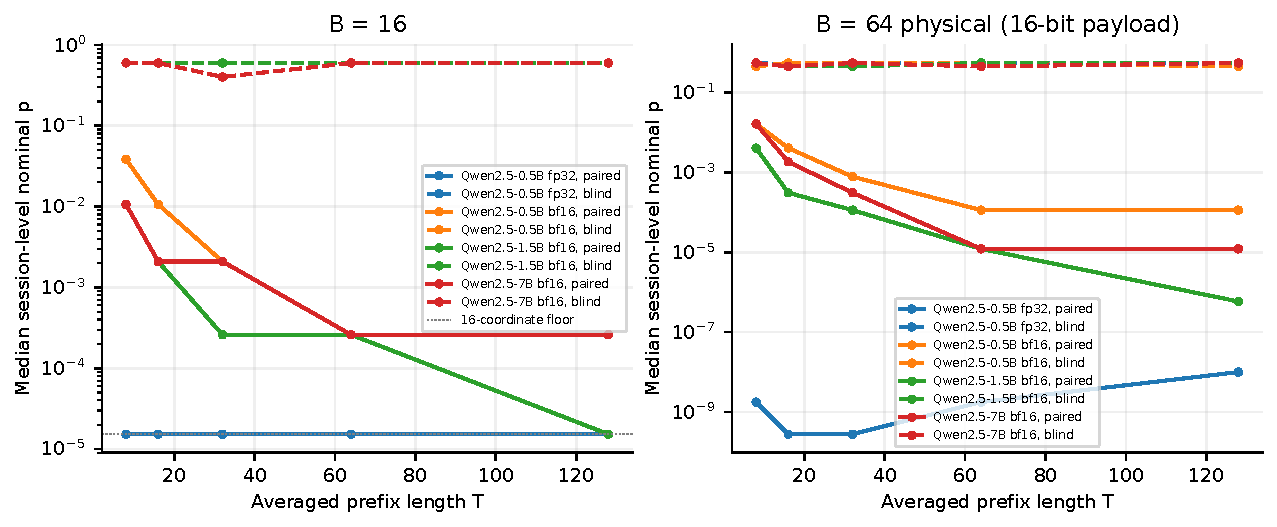
\includegraphics[width=\linewidth]{figures/p_vs_T.pdf}
\caption{Median session-level nominal detection tails for sixteen and sixty-four physical coordinates. Solid: paired; dashed: blind. The sixteen-coordinate floor applies only to the left panel.}\label{fig:curve}
\end{figure}
% Generated by make_tables.py; do not edit.
\begin{table}[htbp]
\centering
\small
\resizebox{\textwidth}{!}{%
\begin{tabular}{lrrrrrrr}
\toprule
Model/dtype & Coordinates & Mode & $T=8$ & $T=16$ & $T=32$ & $T=64$ & $T=128$ \\
\midrule
0.5B fp32 & $16$ phys. & paired & $\csname R0B16pairedTp8\endcsname$ & $\csname R0B16pairedTp16\endcsname$ & $\csname R0B16pairedTp32\endcsname$ & $\csname R0B16pairedTp64\endcsname$ & $\csname R0B16pairedTp128\endcsname$ \\
0.5B fp32 & $16$ phys. & blind & $\csname R0B16blindTp8\endcsname$ & $\csname R0B16blindTp16\endcsname$ & $\csname R0B16blindTp32\endcsname$ & $\csname R0B16blindTp64\endcsname$ & $\csname R0B16blindTp128\endcsname$ \\
0.5B fp32 & $64$ phys. & paired & $\csname R0B64PhyspairedTp8\endcsname$ & $\csname R0B64PhyspairedTp16\endcsname$ & $\csname R0B64PhyspairedTp32\endcsname$ & $\csname R0B64PhyspairedTp64\endcsname$ & $\csname R0B64PhyspairedTp128\endcsname$ \\
0.5B fp32 & $64$ phys. & blind & $\csname R0B64PhysblindTp8\endcsname$ & $\csname R0B64PhysblindTp16\endcsname$ & $\csname R0B64PhysblindTp32\endcsname$ & $\csname R0B64PhysblindTp64\endcsname$ & $\csname R0B64PhysblindTp128\endcsname$ \\
0.5B fp32 & $16$ log. ($64$) & paired & $\csname R0B64pairedTp8\endcsname$ & $\csname R0B64pairedTp16\endcsname$ & $\csname R0B64pairedTp32\endcsname$ & $\csname R0B64pairedTp64\endcsname$ & $\csname R0B64pairedTp128\endcsname$ \\
0.5B fp32 & $16$ log. ($64$) & blind & $\csname R0B64blindTp8\endcsname$ & $\csname R0B64blindTp16\endcsname$ & $\csname R0B64blindTp32\endcsname$ & $\csname R0B64blindTp64\endcsname$ & $\csname R0B64blindTp128\endcsname$ \\
0.5B bf16 & $16$ phys. & paired & $\csname R1B16pairedTp8\endcsname$ & $\csname R1B16pairedTp16\endcsname$ & $\csname R1B16pairedTp32\endcsname$ & $\csname R1B16pairedTp64\endcsname$ & $\csname R1B16pairedTp128\endcsname$ \\
0.5B bf16 & $16$ phys. & blind & $\csname R1B16blindTp8\endcsname$ & $\csname R1B16blindTp16\endcsname$ & $\csname R1B16blindTp32\endcsname$ & $\csname R1B16blindTp64\endcsname$ & $\csname R1B16blindTp128\endcsname$ \\
0.5B bf16 & $64$ phys. & paired & $\csname R1B64PhyspairedTp8\endcsname$ & $\csname R1B64PhyspairedTp16\endcsname$ & $\csname R1B64PhyspairedTp32\endcsname$ & $\csname R1B64PhyspairedTp64\endcsname$ & $\csname R1B64PhyspairedTp128\endcsname$ \\
0.5B bf16 & $64$ phys. & blind & $\csname R1B64PhysblindTp8\endcsname$ & $\csname R1B64PhysblindTp16\endcsname$ & $\csname R1B64PhysblindTp32\endcsname$ & $\csname R1B64PhysblindTp64\endcsname$ & $\csname R1B64PhysblindTp128\endcsname$ \\
0.5B bf16 & $16$ log. ($64$) & paired & $\csname R1B64pairedTp8\endcsname$ & $\csname R1B64pairedTp16\endcsname$ & $\csname R1B64pairedTp32\endcsname$ & $\csname R1B64pairedTp64\endcsname$ & $\csname R1B64pairedTp128\endcsname$ \\
0.5B bf16 & $16$ log. ($64$) & blind & $\csname R1B64blindTp8\endcsname$ & $\csname R1B64blindTp16\endcsname$ & $\csname R1B64blindTp32\endcsname$ & $\csname R1B64blindTp64\endcsname$ & $\csname R1B64blindTp128\endcsname$ \\
1.5B bf16 & $16$ phys. & paired & $\csname R2B16pairedTp8\endcsname$ & $\csname R2B16pairedTp16\endcsname$ & $\csname R2B16pairedTp32\endcsname$ & $\csname R2B16pairedTp64\endcsname$ & $\csname R2B16pairedTp128\endcsname$ \\
1.5B bf16 & $16$ phys. & blind & $\csname R2B16blindTp8\endcsname$ & $\csname R2B16blindTp16\endcsname$ & $\csname R2B16blindTp32\endcsname$ & $\csname R2B16blindTp64\endcsname$ & $\csname R2B16blindTp128\endcsname$ \\
1.5B bf16 & $64$ phys. & paired & $\csname R2B64PhyspairedTp8\endcsname$ & $\csname R2B64PhyspairedTp16\endcsname$ & $\csname R2B64PhyspairedTp32\endcsname$ & $\csname R2B64PhyspairedTp64\endcsname$ & $\csname R2B64PhyspairedTp128\endcsname$ \\
1.5B bf16 & $64$ phys. & blind & $\csname R2B64PhysblindTp8\endcsname$ & $\csname R2B64PhysblindTp16\endcsname$ & $\csname R2B64PhysblindTp32\endcsname$ & $\csname R2B64PhysblindTp64\endcsname$ & $\csname R2B64PhysblindTp128\endcsname$ \\
1.5B bf16 & $16$ log. ($64$) & paired & $\csname R2B64pairedTp8\endcsname$ & $\csname R2B64pairedTp16\endcsname$ & $\csname R2B64pairedTp32\endcsname$ & $\csname R2B64pairedTp64\endcsname$ & $\csname R2B64pairedTp128\endcsname$ \\
1.5B bf16 & $16$ log. ($64$) & blind & $\csname R2B64blindTp8\endcsname$ & $\csname R2B64blindTp16\endcsname$ & $\csname R2B64blindTp32\endcsname$ & $\csname R2B64blindTp64\endcsname$ & $\csname R2B64blindTp128\endcsname$ \\
7B bf16 & $16$ phys. & paired & $\csname R3B16pairedTp8\endcsname$ & $\csname R3B16pairedTp16\endcsname$ & $\csname R3B16pairedTp32\endcsname$ & $\csname R3B16pairedTp64\endcsname$ & $\csname R3B16pairedTp128\endcsname$ \\
7B bf16 & $16$ phys. & blind & $\csname R3B16blindTp8\endcsname$ & $\csname R3B16blindTp16\endcsname$ & $\csname R3B16blindTp32\endcsname$ & $\csname R3B16blindTp64\endcsname$ & $\csname R3B16blindTp128\endcsname$ \\
7B bf16 & $64$ phys. & paired & $\csname R3B64PhyspairedTp8\endcsname$ & $\csname R3B64PhyspairedTp16\endcsname$ & $\csname R3B64PhyspairedTp32\endcsname$ & $\csname R3B64PhyspairedTp64\endcsname$ & $\csname R3B64PhyspairedTp128\endcsname$ \\
7B bf16 & $64$ phys. & blind & $\csname R3B64PhysblindTp8\endcsname$ & $\csname R3B64PhysblindTp16\endcsname$ & $\csname R3B64PhysblindTp32\endcsname$ & $\csname R3B64PhysblindTp64\endcsname$ & $\csname R3B64PhysblindTp128\endcsname$ \\
7B bf16 & $16$ log. ($64$) & paired & $\csname R3B64pairedTp8\endcsname$ & $\csname R3B64pairedTp16\endcsname$ & $\csname R3B64pairedTp32\endcsname$ & $\csname R3B64pairedTp64\endcsname$ & $\csname R3B64pairedTp128\endcsname$ \\
7B bf16 & $16$ log. ($64$) & blind & $\csname R3B64blindTp8\endcsname$ & $\csname R3B64blindTp16\endcsname$ & $\csname R3B64blindTp32\endcsname$ & $\csname R3B64blindTp64\endcsname$ & $\csname R3B64blindTp128\endcsname$ \\
\bottomrule
\end{tabular}
}
\caption{Median session-level nominal tails versus prefix length. Physical and logical statistics are separated; logical prefix tails are reconstructed from session records.}\label{tab:curve}
\end{table}


\subsection{Null controls and substitution}
\ControlResults
These rates fluctuate around low null exceedance rates; the occasional rate above
nominal does not establish a calibrated bound. Zero observed exceedances cannot
validate a $10^{-5}$ false-positive guarantee with only $128$ sessions per series.
The physical controls test the null required by Eq.~\eqref{eq:p}; repetition is
not a reason to discard those coordinates.
Paired no-mark directly measures the empirical FPR of the recommended verifier,
including cached-generation versus full-replay numerical differences.
\PairedNoMarkResults{}
Pending paired no-mark conditions: \PairedNoMarkPending.
% Generated by make_tables.py; do not edit.
\begin{table}[htbp]
\centering
\small
\resizebox{\textwidth}{!}{%
\begin{tabular}{lrrrrrrrrr}
\toprule
Model/dtype & $B$ & Control/mode & Bit acc. & Matches & Nominal median $p$ & $<10^{-2}$ & $<10^{-3}$ & $<10^{-4}$ & $<10^{-5}$ \\
\midrule
0.5B fp32 & $16$ phys. & wrong 1, paired & $\csname R0B16wrong1pairedacc\endcsname$ & $\csname R0B16wrong1pairedmatches\endcsname$ & $\csname R0B16wrong1pairedp\endcsname$ & $\csname R0B16wrong1pairedfrac0\endcsname$ & $\csname R0B16wrong1pairedfrac1\endcsname$ & $\csname R0B16wrong1pairedfrac2\endcsname$ & $\csname R0B16wrong1pairedfrac3\endcsname$ \\
0.5B fp32 & $16$ phys. & wrong 1, blind & $\csname R0B16wrong1blindacc\endcsname$ & $\csname R0B16wrong1blindmatches\endcsname$ & $\csname R0B16wrong1blindp\endcsname$ & $\csname R0B16wrong1blindfrac0\endcsname$ & $\csname R0B16wrong1blindfrac1\endcsname$ & $\csname R0B16wrong1blindfrac2\endcsname$ & $\csname R0B16wrong1blindfrac3\endcsname$ \\
0.5B fp32 & $16$ phys. & wrong 2, paired & $\csname R0B16wrong2pairedacc\endcsname$ & $\csname R0B16wrong2pairedmatches\endcsname$ & $\csname R0B16wrong2pairedp\endcsname$ & $\csname R0B16wrong2pairedfrac0\endcsname$ & $\csname R0B16wrong2pairedfrac1\endcsname$ & $\csname R0B16wrong2pairedfrac2\endcsname$ & $\csname R0B16wrong2pairedfrac3\endcsname$ \\
0.5B fp32 & $16$ phys. & wrong 2, blind & $\csname R0B16wrong2blindacc\endcsname$ & $\csname R0B16wrong2blindmatches\endcsname$ & $\csname R0B16wrong2blindp\endcsname$ & $\csname R0B16wrong2blindfrac0\endcsname$ & $\csname R0B16wrong2blindfrac1\endcsname$ & $\csname R0B16wrong2blindfrac2\endcsname$ & $\csname R0B16wrong2blindfrac3\endcsname$ \\
0.5B fp32 & $16$ phys. & nomark blind & $\csname R0B16nomark_blindacc\endcsname$ & $\csname R0B16nomark_blindmatches\endcsname$ & $\csname R0B16nomark_blindp\endcsname$ & $\csname R0B16nomark_blindfrac0\endcsname$ & $\csname R0B16nomark_blindfrac1\endcsname$ & $\csname R0B16nomark_blindfrac2\endcsname$ & $\csname R0B16nomark_blindfrac3\endcsname$ \\
0.5B fp32 & $16$ phys. & substitution paired & $\csname R0B16substitution_pairedacc\endcsname$ & $\csname R0B16substitution_pairedmatches\endcsname$ & $\csname R0B16substitution_pairedp\endcsname$ & $\csname R0B16substitution_pairedfrac0\endcsname$ & $\csname R0B16substitution_pairedfrac1\endcsname$ & $\csname R0B16substitution_pairedfrac2\endcsname$ & $\csname R0B16substitution_pairedfrac3\endcsname$ \\
0.5B fp32 & $16$ phys. & substitution blind & $\csname R0B16substitution_blindacc\endcsname$ & $\csname R0B16substitution_blindmatches\endcsname$ & $\csname R0B16substitution_blindp\endcsname$ & $\csname R0B16substitution_blindfrac0\endcsname$ & $\csname R0B16substitution_blindfrac1\endcsname$ & $\csname R0B16substitution_blindfrac2\endcsname$ & $\csname R0B16substitution_blindfrac3\endcsname$ \\
0.5B fp32 & $16$ phys. & no-mark, paired & $\csname R0B16nomark_pairedacc\endcsname$ & $\csname R0B16nomark_pairedmatches\endcsname$ & $\csname R0B16nomark_pairedp\endcsname$ & $\csname R0B16nomark_pairedfrac0\endcsname$ & $\csname R0B16nomark_pairedfrac1\endcsname$ & $\csname R0B16nomark_pairedfrac2\endcsname$ & $\csname R0B16nomark_pairedfrac3\endcsname$ \\
0.5B fp32 & $64$ phys. & wrong 1, paired & $\csname R0B64Physwrong1pairedacc\endcsname$ & $\csname R0B64Physwrong1pairedmatches\endcsname$ & $\csname R0B64Physwrong1pairedp\endcsname$ & $\csname R0B64Physwrong1pairedfrac0\endcsname$ & $\csname R0B64Physwrong1pairedfrac1\endcsname$ & $\csname R0B64Physwrong1pairedfrac2\endcsname$ & $\csname R0B64Physwrong1pairedfrac3\endcsname$ \\
0.5B fp32 & $64$ phys. & wrong 1, blind & $\csname R0B64Physwrong1blindacc\endcsname$ & $\csname R0B64Physwrong1blindmatches\endcsname$ & $\csname R0B64Physwrong1blindp\endcsname$ & $\csname R0B64Physwrong1blindfrac0\endcsname$ & $\csname R0B64Physwrong1blindfrac1\endcsname$ & $\csname R0B64Physwrong1blindfrac2\endcsname$ & $\csname R0B64Physwrong1blindfrac3\endcsname$ \\
0.5B fp32 & $64$ phys. & wrong 2, paired & $\csname R0B64Physwrong2pairedacc\endcsname$ & $\csname R0B64Physwrong2pairedmatches\endcsname$ & $\csname R0B64Physwrong2pairedp\endcsname$ & $\csname R0B64Physwrong2pairedfrac0\endcsname$ & $\csname R0B64Physwrong2pairedfrac1\endcsname$ & $\csname R0B64Physwrong2pairedfrac2\endcsname$ & $\csname R0B64Physwrong2pairedfrac3\endcsname$ \\
0.5B fp32 & $64$ phys. & wrong 2, blind & $\csname R0B64Physwrong2blindacc\endcsname$ & $\csname R0B64Physwrong2blindmatches\endcsname$ & $\csname R0B64Physwrong2blindp\endcsname$ & $\csname R0B64Physwrong2blindfrac0\endcsname$ & $\csname R0B64Physwrong2blindfrac1\endcsname$ & $\csname R0B64Physwrong2blindfrac2\endcsname$ & $\csname R0B64Physwrong2blindfrac3\endcsname$ \\
0.5B fp32 & $64$ phys. & nomark blind & $\csname R0B64Physnomark_blindacc\endcsname$ & $\csname R0B64Physnomark_blindmatches\endcsname$ & $\csname R0B64Physnomark_blindp\endcsname$ & $\csname R0B64Physnomark_blindfrac0\endcsname$ & $\csname R0B64Physnomark_blindfrac1\endcsname$ & $\csname R0B64Physnomark_blindfrac2\endcsname$ & $\csname R0B64Physnomark_blindfrac3\endcsname$ \\
0.5B fp32 & $64$ phys. & substitution paired & $\csname R0B64Physsubstitution_pairedacc\endcsname$ & $\csname R0B64Physsubstitution_pairedmatches\endcsname$ & $\csname R0B64Physsubstitution_pairedp\endcsname$ & $\csname R0B64Physsubstitution_pairedfrac0\endcsname$ & $\csname R0B64Physsubstitution_pairedfrac1\endcsname$ & $\csname R0B64Physsubstitution_pairedfrac2\endcsname$ & $\csname R0B64Physsubstitution_pairedfrac3\endcsname$ \\
0.5B fp32 & $64$ phys. & substitution blind & $\csname R0B64Physsubstitution_blindacc\endcsname$ & $\csname R0B64Physsubstitution_blindmatches\endcsname$ & $\csname R0B64Physsubstitution_blindp\endcsname$ & $\csname R0B64Physsubstitution_blindfrac0\endcsname$ & $\csname R0B64Physsubstitution_blindfrac1\endcsname$ & $\csname R0B64Physsubstitution_blindfrac2\endcsname$ & $\csname R0B64Physsubstitution_blindfrac3\endcsname$ \\
0.5B fp32 & $64$ phys. & no-mark, paired & $\csname R0B64Physnomark_pairedacc\endcsname$ & $\csname R0B64Physnomark_pairedmatches\endcsname$ & $\csname R0B64Physnomark_pairedp\endcsname$ & $\csname R0B64Physnomark_pairedfrac0\endcsname$ & $\csname R0B64Physnomark_pairedfrac1\endcsname$ & $\csname R0B64Physnomark_pairedfrac2\endcsname$ & $\csname R0B64Physnomark_pairedfrac3\endcsname$ \\
0.5B fp32 & $16$ log. ($64$) & wrong 1, paired & $\csname R0B64wrong1pairedacc\endcsname$ & $\csname R0B64wrong1pairedmatches\endcsname$ & $\csname R0B64wrong1pairedp\endcsname$ & $\csname R0B64wrong1pairedfrac0\endcsname$ & $\csname R0B64wrong1pairedfrac1\endcsname$ & $\csname R0B64wrong1pairedfrac2\endcsname$ & $\csname R0B64wrong1pairedfrac3\endcsname$ \\
0.5B fp32 & $16$ log. ($64$) & wrong 1, blind & $\csname R0B64wrong1blindacc\endcsname$ & $\csname R0B64wrong1blindmatches\endcsname$ & $\csname R0B64wrong1blindp\endcsname$ & $\csname R0B64wrong1blindfrac0\endcsname$ & $\csname R0B64wrong1blindfrac1\endcsname$ & $\csname R0B64wrong1blindfrac2\endcsname$ & $\csname R0B64wrong1blindfrac3\endcsname$ \\
0.5B fp32 & $16$ log. ($64$) & wrong 2, paired & $\csname R0B64wrong2pairedacc\endcsname$ & $\csname R0B64wrong2pairedmatches\endcsname$ & $\csname R0B64wrong2pairedp\endcsname$ & $\csname R0B64wrong2pairedfrac0\endcsname$ & $\csname R0B64wrong2pairedfrac1\endcsname$ & $\csname R0B64wrong2pairedfrac2\endcsname$ & $\csname R0B64wrong2pairedfrac3\endcsname$ \\
0.5B fp32 & $16$ log. ($64$) & wrong 2, blind & $\csname R0B64wrong2blindacc\endcsname$ & $\csname R0B64wrong2blindmatches\endcsname$ & $\csname R0B64wrong2blindp\endcsname$ & $\csname R0B64wrong2blindfrac0\endcsname$ & $\csname R0B64wrong2blindfrac1\endcsname$ & $\csname R0B64wrong2blindfrac2\endcsname$ & $\csname R0B64wrong2blindfrac3\endcsname$ \\
0.5B fp32 & $16$ log. ($64$) & nomark blind & $\csname R0B64nomark_blindacc\endcsname$ & $\csname R0B64nomark_blindmatches\endcsname$ & $\csname R0B64nomark_blindp\endcsname$ & $\csname R0B64nomark_blindfrac0\endcsname$ & $\csname R0B64nomark_blindfrac1\endcsname$ & $\csname R0B64nomark_blindfrac2\endcsname$ & $\csname R0B64nomark_blindfrac3\endcsname$ \\
0.5B fp32 & $16$ log. ($64$) & substitution paired & $\csname R0B64substitution_pairedacc\endcsname$ & $\csname R0B64substitution_pairedmatches\endcsname$ & $\csname R0B64substitution_pairedp\endcsname$ & $\csname R0B64substitution_pairedfrac0\endcsname$ & $\csname R0B64substitution_pairedfrac1\endcsname$ & $\csname R0B64substitution_pairedfrac2\endcsname$ & $\csname R0B64substitution_pairedfrac3\endcsname$ \\
0.5B fp32 & $16$ log. ($64$) & substitution blind & $\csname R0B64substitution_blindacc\endcsname$ & $\csname R0B64substitution_blindmatches\endcsname$ & $\csname R0B64substitution_blindp\endcsname$ & $\csname R0B64substitution_blindfrac0\endcsname$ & $\csname R0B64substitution_blindfrac1\endcsname$ & $\csname R0B64substitution_blindfrac2\endcsname$ & $\csname R0B64substitution_blindfrac3\endcsname$ \\
0.5B fp32 & $16$ log. ($64$) & no-mark, paired & $\csname R0B64nomark_pairedacc\endcsname$ & $\csname R0B64nomark_pairedmatches\endcsname$ & $\csname R0B64nomark_pairedp\endcsname$ & $\csname R0B64nomark_pairedfrac0\endcsname$ & $\csname R0B64nomark_pairedfrac1\endcsname$ & $\csname R0B64nomark_pairedfrac2\endcsname$ & $\csname R0B64nomark_pairedfrac3\endcsname$ \\
0.5B bf16 & $16$ phys. & wrong 1, paired & $\csname R1B16wrong1pairedacc\endcsname$ & $\csname R1B16wrong1pairedmatches\endcsname$ & $\csname R1B16wrong1pairedp\endcsname$ & $\csname R1B16wrong1pairedfrac0\endcsname$ & $\csname R1B16wrong1pairedfrac1\endcsname$ & $\csname R1B16wrong1pairedfrac2\endcsname$ & $\csname R1B16wrong1pairedfrac3\endcsname$ \\
0.5B bf16 & $16$ phys. & wrong 1, blind & $\csname R1B16wrong1blindacc\endcsname$ & $\csname R1B16wrong1blindmatches\endcsname$ & $\csname R1B16wrong1blindp\endcsname$ & $\csname R1B16wrong1blindfrac0\endcsname$ & $\csname R1B16wrong1blindfrac1\endcsname$ & $\csname R1B16wrong1blindfrac2\endcsname$ & $\csname R1B16wrong1blindfrac3\endcsname$ \\
0.5B bf16 & $16$ phys. & wrong 2, paired & $\csname R1B16wrong2pairedacc\endcsname$ & $\csname R1B16wrong2pairedmatches\endcsname$ & $\csname R1B16wrong2pairedp\endcsname$ & $\csname R1B16wrong2pairedfrac0\endcsname$ & $\csname R1B16wrong2pairedfrac1\endcsname$ & $\csname R1B16wrong2pairedfrac2\endcsname$ & $\csname R1B16wrong2pairedfrac3\endcsname$ \\
0.5B bf16 & $16$ phys. & wrong 2, blind & $\csname R1B16wrong2blindacc\endcsname$ & $\csname R1B16wrong2blindmatches\endcsname$ & $\csname R1B16wrong2blindp\endcsname$ & $\csname R1B16wrong2blindfrac0\endcsname$ & $\csname R1B16wrong2blindfrac1\endcsname$ & $\csname R1B16wrong2blindfrac2\endcsname$ & $\csname R1B16wrong2blindfrac3\endcsname$ \\
0.5B bf16 & $16$ phys. & nomark blind & $\csname R1B16nomark_blindacc\endcsname$ & $\csname R1B16nomark_blindmatches\endcsname$ & $\csname R1B16nomark_blindp\endcsname$ & $\csname R1B16nomark_blindfrac0\endcsname$ & $\csname R1B16nomark_blindfrac1\endcsname$ & $\csname R1B16nomark_blindfrac2\endcsname$ & $\csname R1B16nomark_blindfrac3\endcsname$ \\
0.5B bf16 & $16$ phys. & substitution paired & $\csname R1B16substitution_pairedacc\endcsname$ & $\csname R1B16substitution_pairedmatches\endcsname$ & $\csname R1B16substitution_pairedp\endcsname$ & $\csname R1B16substitution_pairedfrac0\endcsname$ & $\csname R1B16substitution_pairedfrac1\endcsname$ & $\csname R1B16substitution_pairedfrac2\endcsname$ & $\csname R1B16substitution_pairedfrac3\endcsname$ \\
0.5B bf16 & $16$ phys. & substitution blind & $\csname R1B16substitution_blindacc\endcsname$ & $\csname R1B16substitution_blindmatches\endcsname$ & $\csname R1B16substitution_blindp\endcsname$ & $\csname R1B16substitution_blindfrac0\endcsname$ & $\csname R1B16substitution_blindfrac1\endcsname$ & $\csname R1B16substitution_blindfrac2\endcsname$ & $\csname R1B16substitution_blindfrac3\endcsname$ \\
0.5B bf16 & $16$ phys. & no-mark, paired & $\csname R1B16nomark_pairedacc\endcsname$ & $\csname R1B16nomark_pairedmatches\endcsname$ & $\csname R1B16nomark_pairedp\endcsname$ & $\csname R1B16nomark_pairedfrac0\endcsname$ & $\csname R1B16nomark_pairedfrac1\endcsname$ & $\csname R1B16nomark_pairedfrac2\endcsname$ & $\csname R1B16nomark_pairedfrac3\endcsname$ \\
\bottomrule
\end{tabular}
}
\caption{Null and substitution controls, including sixty-four-physical-bit detection and sixteen-logical-bit recovery. No-mark threshold columns are empirical FPRs; paired rows appear when measured. All tails are nominal; logical tails are nominal (payload-randomised). Wrong keys are fixed controls.}\label{tab:controls}
\end{table}

% Generated by make_tables.py; do not edit.
\begin{table}[htbp]
\centering
\small
\resizebox{\textwidth}{!}{%
\begin{tabular}{lrrrrrrrrr}
\toprule
Model/dtype & $B$ & Control/mode & Bit acc. & Matches & Nominal median $p$ & $<10^{-2}$ & $<10^{-3}$ & $<10^{-4}$ & $<10^{-5}$ \\
\midrule
0.5B bf16 & $64$ phys. & wrong 1, paired & $\csname R1B64Physwrong1pairedacc\endcsname$ & $\csname R1B64Physwrong1pairedmatches\endcsname$ & $\csname R1B64Physwrong1pairedp\endcsname$ & $\csname R1B64Physwrong1pairedfrac0\endcsname$ & $\csname R1B64Physwrong1pairedfrac1\endcsname$ & $\csname R1B64Physwrong1pairedfrac2\endcsname$ & $\csname R1B64Physwrong1pairedfrac3\endcsname$ \\
0.5B bf16 & $64$ phys. & wrong 1, blind & $\csname R1B64Physwrong1blindacc\endcsname$ & $\csname R1B64Physwrong1blindmatches\endcsname$ & $\csname R1B64Physwrong1blindp\endcsname$ & $\csname R1B64Physwrong1blindfrac0\endcsname$ & $\csname R1B64Physwrong1blindfrac1\endcsname$ & $\csname R1B64Physwrong1blindfrac2\endcsname$ & $\csname R1B64Physwrong1blindfrac3\endcsname$ \\
0.5B bf16 & $64$ phys. & wrong 2, paired & $\csname R1B64Physwrong2pairedacc\endcsname$ & $\csname R1B64Physwrong2pairedmatches\endcsname$ & $\csname R1B64Physwrong2pairedp\endcsname$ & $\csname R1B64Physwrong2pairedfrac0\endcsname$ & $\csname R1B64Physwrong2pairedfrac1\endcsname$ & $\csname R1B64Physwrong2pairedfrac2\endcsname$ & $\csname R1B64Physwrong2pairedfrac3\endcsname$ \\
0.5B bf16 & $64$ phys. & wrong 2, blind & $\csname R1B64Physwrong2blindacc\endcsname$ & $\csname R1B64Physwrong2blindmatches\endcsname$ & $\csname R1B64Physwrong2blindp\endcsname$ & $\csname R1B64Physwrong2blindfrac0\endcsname$ & $\csname R1B64Physwrong2blindfrac1\endcsname$ & $\csname R1B64Physwrong2blindfrac2\endcsname$ & $\csname R1B64Physwrong2blindfrac3\endcsname$ \\
0.5B bf16 & $64$ phys. & nomark blind & $\csname R1B64Physnomark_blindacc\endcsname$ & $\csname R1B64Physnomark_blindmatches\endcsname$ & $\csname R1B64Physnomark_blindp\endcsname$ & $\csname R1B64Physnomark_blindfrac0\endcsname$ & $\csname R1B64Physnomark_blindfrac1\endcsname$ & $\csname R1B64Physnomark_blindfrac2\endcsname$ & $\csname R1B64Physnomark_blindfrac3\endcsname$ \\
0.5B bf16 & $64$ phys. & substitution paired & $\csname R1B64Physsubstitution_pairedacc\endcsname$ & $\csname R1B64Physsubstitution_pairedmatches\endcsname$ & $\csname R1B64Physsubstitution_pairedp\endcsname$ & $\csname R1B64Physsubstitution_pairedfrac0\endcsname$ & $\csname R1B64Physsubstitution_pairedfrac1\endcsname$ & $\csname R1B64Physsubstitution_pairedfrac2\endcsname$ & $\csname R1B64Physsubstitution_pairedfrac3\endcsname$ \\
0.5B bf16 & $64$ phys. & substitution blind & $\csname R1B64Physsubstitution_blindacc\endcsname$ & $\csname R1B64Physsubstitution_blindmatches\endcsname$ & $\csname R1B64Physsubstitution_blindp\endcsname$ & $\csname R1B64Physsubstitution_blindfrac0\endcsname$ & $\csname R1B64Physsubstitution_blindfrac1\endcsname$ & $\csname R1B64Physsubstitution_blindfrac2\endcsname$ & $\csname R1B64Physsubstitution_blindfrac3\endcsname$ \\
0.5B bf16 & $64$ phys. & no-mark, paired & $\csname R1B64Physnomark_pairedacc\endcsname$ & $\csname R1B64Physnomark_pairedmatches\endcsname$ & $\csname R1B64Physnomark_pairedp\endcsname$ & $\csname R1B64Physnomark_pairedfrac0\endcsname$ & $\csname R1B64Physnomark_pairedfrac1\endcsname$ & $\csname R1B64Physnomark_pairedfrac2\endcsname$ & $\csname R1B64Physnomark_pairedfrac3\endcsname$ \\
0.5B bf16 & $16$ log. ($64$) & wrong 1, paired & $\csname R1B64wrong1pairedacc\endcsname$ & $\csname R1B64wrong1pairedmatches\endcsname$ & $\csname R1B64wrong1pairedp\endcsname$ & $\csname R1B64wrong1pairedfrac0\endcsname$ & $\csname R1B64wrong1pairedfrac1\endcsname$ & $\csname R1B64wrong1pairedfrac2\endcsname$ & $\csname R1B64wrong1pairedfrac3\endcsname$ \\
0.5B bf16 & $16$ log. ($64$) & wrong 1, blind & $\csname R1B64wrong1blindacc\endcsname$ & $\csname R1B64wrong1blindmatches\endcsname$ & $\csname R1B64wrong1blindp\endcsname$ & $\csname R1B64wrong1blindfrac0\endcsname$ & $\csname R1B64wrong1blindfrac1\endcsname$ & $\csname R1B64wrong1blindfrac2\endcsname$ & $\csname R1B64wrong1blindfrac3\endcsname$ \\
0.5B bf16 & $16$ log. ($64$) & wrong 2, paired & $\csname R1B64wrong2pairedacc\endcsname$ & $\csname R1B64wrong2pairedmatches\endcsname$ & $\csname R1B64wrong2pairedp\endcsname$ & $\csname R1B64wrong2pairedfrac0\endcsname$ & $\csname R1B64wrong2pairedfrac1\endcsname$ & $\csname R1B64wrong2pairedfrac2\endcsname$ & $\csname R1B64wrong2pairedfrac3\endcsname$ \\
0.5B bf16 & $16$ log. ($64$) & wrong 2, blind & $\csname R1B64wrong2blindacc\endcsname$ & $\csname R1B64wrong2blindmatches\endcsname$ & $\csname R1B64wrong2blindp\endcsname$ & $\csname R1B64wrong2blindfrac0\endcsname$ & $\csname R1B64wrong2blindfrac1\endcsname$ & $\csname R1B64wrong2blindfrac2\endcsname$ & $\csname R1B64wrong2blindfrac3\endcsname$ \\
0.5B bf16 & $16$ log. ($64$) & nomark blind & $\csname R1B64nomark_blindacc\endcsname$ & $\csname R1B64nomark_blindmatches\endcsname$ & $\csname R1B64nomark_blindp\endcsname$ & $\csname R1B64nomark_blindfrac0\endcsname$ & $\csname R1B64nomark_blindfrac1\endcsname$ & $\csname R1B64nomark_blindfrac2\endcsname$ & $\csname R1B64nomark_blindfrac3\endcsname$ \\
0.5B bf16 & $16$ log. ($64$) & substitution paired & $\csname R1B64substitution_pairedacc\endcsname$ & $\csname R1B64substitution_pairedmatches\endcsname$ & $\csname R1B64substitution_pairedp\endcsname$ & $\csname R1B64substitution_pairedfrac0\endcsname$ & $\csname R1B64substitution_pairedfrac1\endcsname$ & $\csname R1B64substitution_pairedfrac2\endcsname$ & $\csname R1B64substitution_pairedfrac3\endcsname$ \\
0.5B bf16 & $16$ log. ($64$) & substitution blind & $\csname R1B64substitution_blindacc\endcsname$ & $\csname R1B64substitution_blindmatches\endcsname$ & $\csname R1B64substitution_blindp\endcsname$ & $\csname R1B64substitution_blindfrac0\endcsname$ & $\csname R1B64substitution_blindfrac1\endcsname$ & $\csname R1B64substitution_blindfrac2\endcsname$ & $\csname R1B64substitution_blindfrac3\endcsname$ \\
0.5B bf16 & $16$ log. ($64$) & no-mark, paired & $\csname R1B64nomark_pairedacc\endcsname$ & $\csname R1B64nomark_pairedmatches\endcsname$ & $\csname R1B64nomark_pairedp\endcsname$ & $\csname R1B64nomark_pairedfrac0\endcsname$ & $\csname R1B64nomark_pairedfrac1\endcsname$ & $\csname R1B64nomark_pairedfrac2\endcsname$ & $\csname R1B64nomark_pairedfrac3\endcsname$ \\
1.5B bf16 & $16$ phys. & wrong 1, paired & $\csname R2B16wrong1pairedacc\endcsname$ & $\csname R2B16wrong1pairedmatches\endcsname$ & $\csname R2B16wrong1pairedp\endcsname$ & $\csname R2B16wrong1pairedfrac0\endcsname$ & $\csname R2B16wrong1pairedfrac1\endcsname$ & $\csname R2B16wrong1pairedfrac2\endcsname$ & $\csname R2B16wrong1pairedfrac3\endcsname$ \\
1.5B bf16 & $16$ phys. & wrong 1, blind & $\csname R2B16wrong1blindacc\endcsname$ & $\csname R2B16wrong1blindmatches\endcsname$ & $\csname R2B16wrong1blindp\endcsname$ & $\csname R2B16wrong1blindfrac0\endcsname$ & $\csname R2B16wrong1blindfrac1\endcsname$ & $\csname R2B16wrong1blindfrac2\endcsname$ & $\csname R2B16wrong1blindfrac3\endcsname$ \\
1.5B bf16 & $16$ phys. & wrong 2, paired & $\csname R2B16wrong2pairedacc\endcsname$ & $\csname R2B16wrong2pairedmatches\endcsname$ & $\csname R2B16wrong2pairedp\endcsname$ & $\csname R2B16wrong2pairedfrac0\endcsname$ & $\csname R2B16wrong2pairedfrac1\endcsname$ & $\csname R2B16wrong2pairedfrac2\endcsname$ & $\csname R2B16wrong2pairedfrac3\endcsname$ \\
1.5B bf16 & $16$ phys. & wrong 2, blind & $\csname R2B16wrong2blindacc\endcsname$ & $\csname R2B16wrong2blindmatches\endcsname$ & $\csname R2B16wrong2blindp\endcsname$ & $\csname R2B16wrong2blindfrac0\endcsname$ & $\csname R2B16wrong2blindfrac1\endcsname$ & $\csname R2B16wrong2blindfrac2\endcsname$ & $\csname R2B16wrong2blindfrac3\endcsname$ \\
1.5B bf16 & $16$ phys. & nomark blind & $\csname R2B16nomark_blindacc\endcsname$ & $\csname R2B16nomark_blindmatches\endcsname$ & $\csname R2B16nomark_blindp\endcsname$ & $\csname R2B16nomark_blindfrac0\endcsname$ & $\csname R2B16nomark_blindfrac1\endcsname$ & $\csname R2B16nomark_blindfrac2\endcsname$ & $\csname R2B16nomark_blindfrac3\endcsname$ \\
1.5B bf16 & $16$ phys. & substitution paired & $\csname R2B16substitution_pairedacc\endcsname$ & $\csname R2B16substitution_pairedmatches\endcsname$ & $\csname R2B16substitution_pairedp\endcsname$ & $\csname R2B16substitution_pairedfrac0\endcsname$ & $\csname R2B16substitution_pairedfrac1\endcsname$ & $\csname R2B16substitution_pairedfrac2\endcsname$ & $\csname R2B16substitution_pairedfrac3\endcsname$ \\
1.5B bf16 & $16$ phys. & substitution blind & $\csname R2B16substitution_blindacc\endcsname$ & $\csname R2B16substitution_blindmatches\endcsname$ & $\csname R2B16substitution_blindp\endcsname$ & $\csname R2B16substitution_blindfrac0\endcsname$ & $\csname R2B16substitution_blindfrac1\endcsname$ & $\csname R2B16substitution_blindfrac2\endcsname$ & $\csname R2B16substitution_blindfrac3\endcsname$ \\
1.5B bf16 & $16$ phys. & no-mark, paired & $\csname R2B16nomark_pairedacc\endcsname$ & $\csname R2B16nomark_pairedmatches\endcsname$ & $\csname R2B16nomark_pairedp\endcsname$ & $\csname R2B16nomark_pairedfrac0\endcsname$ & $\csname R2B16nomark_pairedfrac1\endcsname$ & $\csname R2B16nomark_pairedfrac2\endcsname$ & $\csname R2B16nomark_pairedfrac3\endcsname$ \\
1.5B bf16 & $64$ phys. & wrong 1, paired & $\csname R2B64Physwrong1pairedacc\endcsname$ & $\csname R2B64Physwrong1pairedmatches\endcsname$ & $\csname R2B64Physwrong1pairedp\endcsname$ & $\csname R2B64Physwrong1pairedfrac0\endcsname$ & $\csname R2B64Physwrong1pairedfrac1\endcsname$ & $\csname R2B64Physwrong1pairedfrac2\endcsname$ & $\csname R2B64Physwrong1pairedfrac3\endcsname$ \\
1.5B bf16 & $64$ phys. & wrong 1, blind & $\csname R2B64Physwrong1blindacc\endcsname$ & $\csname R2B64Physwrong1blindmatches\endcsname$ & $\csname R2B64Physwrong1blindp\endcsname$ & $\csname R2B64Physwrong1blindfrac0\endcsname$ & $\csname R2B64Physwrong1blindfrac1\endcsname$ & $\csname R2B64Physwrong1blindfrac2\endcsname$ & $\csname R2B64Physwrong1blindfrac3\endcsname$ \\
1.5B bf16 & $64$ phys. & wrong 2, paired & $\csname R2B64Physwrong2pairedacc\endcsname$ & $\csname R2B64Physwrong2pairedmatches\endcsname$ & $\csname R2B64Physwrong2pairedp\endcsname$ & $\csname R2B64Physwrong2pairedfrac0\endcsname$ & $\csname R2B64Physwrong2pairedfrac1\endcsname$ & $\csname R2B64Physwrong2pairedfrac2\endcsname$ & $\csname R2B64Physwrong2pairedfrac3\endcsname$ \\
1.5B bf16 & $64$ phys. & wrong 2, blind & $\csname R2B64Physwrong2blindacc\endcsname$ & $\csname R2B64Physwrong2blindmatches\endcsname$ & $\csname R2B64Physwrong2blindp\endcsname$ & $\csname R2B64Physwrong2blindfrac0\endcsname$ & $\csname R2B64Physwrong2blindfrac1\endcsname$ & $\csname R2B64Physwrong2blindfrac2\endcsname$ & $\csname R2B64Physwrong2blindfrac3\endcsname$ \\
1.5B bf16 & $64$ phys. & nomark blind & $\csname R2B64Physnomark_blindacc\endcsname$ & $\csname R2B64Physnomark_blindmatches\endcsname$ & $\csname R2B64Physnomark_blindp\endcsname$ & $\csname R2B64Physnomark_blindfrac0\endcsname$ & $\csname R2B64Physnomark_blindfrac1\endcsname$ & $\csname R2B64Physnomark_blindfrac2\endcsname$ & $\csname R2B64Physnomark_blindfrac3\endcsname$ \\
1.5B bf16 & $64$ phys. & substitution paired & $\csname R2B64Physsubstitution_pairedacc\endcsname$ & $\csname R2B64Physsubstitution_pairedmatches\endcsname$ & $\csname R2B64Physsubstitution_pairedp\endcsname$ & $\csname R2B64Physsubstitution_pairedfrac0\endcsname$ & $\csname R2B64Physsubstitution_pairedfrac1\endcsname$ & $\csname R2B64Physsubstitution_pairedfrac2\endcsname$ & $\csname R2B64Physsubstitution_pairedfrac3\endcsname$ \\
1.5B bf16 & $64$ phys. & substitution blind & $\csname R2B64Physsubstitution_blindacc\endcsname$ & $\csname R2B64Physsubstitution_blindmatches\endcsname$ & $\csname R2B64Physsubstitution_blindp\endcsname$ & $\csname R2B64Physsubstitution_blindfrac0\endcsname$ & $\csname R2B64Physsubstitution_blindfrac1\endcsname$ & $\csname R2B64Physsubstitution_blindfrac2\endcsname$ & $\csname R2B64Physsubstitution_blindfrac3\endcsname$ \\
1.5B bf16 & $64$ phys. & no-mark, paired & $\csname R2B64Physnomark_pairedacc\endcsname$ & $\csname R2B64Physnomark_pairedmatches\endcsname$ & $\csname R2B64Physnomark_pairedp\endcsname$ & $\csname R2B64Physnomark_pairedfrac0\endcsname$ & $\csname R2B64Physnomark_pairedfrac1\endcsname$ & $\csname R2B64Physnomark_pairedfrac2\endcsname$ & $\csname R2B64Physnomark_pairedfrac3\endcsname$ \\
\bottomrule
\end{tabular}
}
\caption{Null and substitution controls, including sixty-four-physical-bit detection and sixteen-logical-bit recovery. No-mark threshold columns are empirical FPRs; paired rows appear when measured. All tails are nominal; logical tails are nominal (payload-randomised). Wrong keys are fixed controls. Continued.}\label{tab:controls-part1}
\end{table}

% Generated by make_tables.py; do not edit.
\begin{table}[htbp]
\centering
\small
\resizebox{\textwidth}{!}{%
\begin{tabular}{lrrrrrrrrr}
\toprule
Model/dtype & $B$ & Control/mode & Bit acc. & Matches & Nominal median $p$ & $<10^{-2}$ & $<10^{-3}$ & $<10^{-4}$ & $<10^{-5}$ \\
\midrule
1.5B bf16 & $16$ log. ($64$) & wrong 1, paired & $\csname R2B64wrong1pairedacc\endcsname$ & $\csname R2B64wrong1pairedmatches\endcsname$ & $\csname R2B64wrong1pairedp\endcsname$ & $\csname R2B64wrong1pairedfrac0\endcsname$ & $\csname R2B64wrong1pairedfrac1\endcsname$ & $\csname R2B64wrong1pairedfrac2\endcsname$ & $\csname R2B64wrong1pairedfrac3\endcsname$ \\
1.5B bf16 & $16$ log. ($64$) & wrong 1, blind & $\csname R2B64wrong1blindacc\endcsname$ & $\csname R2B64wrong1blindmatches\endcsname$ & $\csname R2B64wrong1blindp\endcsname$ & $\csname R2B64wrong1blindfrac0\endcsname$ & $\csname R2B64wrong1blindfrac1\endcsname$ & $\csname R2B64wrong1blindfrac2\endcsname$ & $\csname R2B64wrong1blindfrac3\endcsname$ \\
1.5B bf16 & $16$ log. ($64$) & wrong 2, paired & $\csname R2B64wrong2pairedacc\endcsname$ & $\csname R2B64wrong2pairedmatches\endcsname$ & $\csname R2B64wrong2pairedp\endcsname$ & $\csname R2B64wrong2pairedfrac0\endcsname$ & $\csname R2B64wrong2pairedfrac1\endcsname$ & $\csname R2B64wrong2pairedfrac2\endcsname$ & $\csname R2B64wrong2pairedfrac3\endcsname$ \\
1.5B bf16 & $16$ log. ($64$) & wrong 2, blind & $\csname R2B64wrong2blindacc\endcsname$ & $\csname R2B64wrong2blindmatches\endcsname$ & $\csname R2B64wrong2blindp\endcsname$ & $\csname R2B64wrong2blindfrac0\endcsname$ & $\csname R2B64wrong2blindfrac1\endcsname$ & $\csname R2B64wrong2blindfrac2\endcsname$ & $\csname R2B64wrong2blindfrac3\endcsname$ \\
1.5B bf16 & $16$ log. ($64$) & nomark blind & $\csname R2B64nomark_blindacc\endcsname$ & $\csname R2B64nomark_blindmatches\endcsname$ & $\csname R2B64nomark_blindp\endcsname$ & $\csname R2B64nomark_blindfrac0\endcsname$ & $\csname R2B64nomark_blindfrac1\endcsname$ & $\csname R2B64nomark_blindfrac2\endcsname$ & $\csname R2B64nomark_blindfrac3\endcsname$ \\
1.5B bf16 & $16$ log. ($64$) & substitution paired & $\csname R2B64substitution_pairedacc\endcsname$ & $\csname R2B64substitution_pairedmatches\endcsname$ & $\csname R2B64substitution_pairedp\endcsname$ & $\csname R2B64substitution_pairedfrac0\endcsname$ & $\csname R2B64substitution_pairedfrac1\endcsname$ & $\csname R2B64substitution_pairedfrac2\endcsname$ & $\csname R2B64substitution_pairedfrac3\endcsname$ \\
1.5B bf16 & $16$ log. ($64$) & substitution blind & $\csname R2B64substitution_blindacc\endcsname$ & $\csname R2B64substitution_blindmatches\endcsname$ & $\csname R2B64substitution_blindp\endcsname$ & $\csname R2B64substitution_blindfrac0\endcsname$ & $\csname R2B64substitution_blindfrac1\endcsname$ & $\csname R2B64substitution_blindfrac2\endcsname$ & $\csname R2B64substitution_blindfrac3\endcsname$ \\
1.5B bf16 & $16$ log. ($64$) & no-mark, paired & $\csname R2B64nomark_pairedacc\endcsname$ & $\csname R2B64nomark_pairedmatches\endcsname$ & $\csname R2B64nomark_pairedp\endcsname$ & $\csname R2B64nomark_pairedfrac0\endcsname$ & $\csname R2B64nomark_pairedfrac1\endcsname$ & $\csname R2B64nomark_pairedfrac2\endcsname$ & $\csname R2B64nomark_pairedfrac3\endcsname$ \\
7B bf16 & $16$ phys. & wrong 1, paired & $\csname R3B16wrong1pairedacc\endcsname$ & $\csname R3B16wrong1pairedmatches\endcsname$ & $\csname R3B16wrong1pairedp\endcsname$ & $\csname R3B16wrong1pairedfrac0\endcsname$ & $\csname R3B16wrong1pairedfrac1\endcsname$ & $\csname R3B16wrong1pairedfrac2\endcsname$ & $\csname R3B16wrong1pairedfrac3\endcsname$ \\
7B bf16 & $16$ phys. & wrong 1, blind & $\csname R3B16wrong1blindacc\endcsname$ & $\csname R3B16wrong1blindmatches\endcsname$ & $\csname R3B16wrong1blindp\endcsname$ & $\csname R3B16wrong1blindfrac0\endcsname$ & $\csname R3B16wrong1blindfrac1\endcsname$ & $\csname R3B16wrong1blindfrac2\endcsname$ & $\csname R3B16wrong1blindfrac3\endcsname$ \\
7B bf16 & $16$ phys. & wrong 2, paired & $\csname R3B16wrong2pairedacc\endcsname$ & $\csname R3B16wrong2pairedmatches\endcsname$ & $\csname R3B16wrong2pairedp\endcsname$ & $\csname R3B16wrong2pairedfrac0\endcsname$ & $\csname R3B16wrong2pairedfrac1\endcsname$ & $\csname R3B16wrong2pairedfrac2\endcsname$ & $\csname R3B16wrong2pairedfrac3\endcsname$ \\
7B bf16 & $16$ phys. & wrong 2, blind & $\csname R3B16wrong2blindacc\endcsname$ & $\csname R3B16wrong2blindmatches\endcsname$ & $\csname R3B16wrong2blindp\endcsname$ & $\csname R3B16wrong2blindfrac0\endcsname$ & $\csname R3B16wrong2blindfrac1\endcsname$ & $\csname R3B16wrong2blindfrac2\endcsname$ & $\csname R3B16wrong2blindfrac3\endcsname$ \\
7B bf16 & $16$ phys. & nomark blind & $\csname R3B16nomark_blindacc\endcsname$ & $\csname R3B16nomark_blindmatches\endcsname$ & $\csname R3B16nomark_blindp\endcsname$ & $\csname R3B16nomark_blindfrac0\endcsname$ & $\csname R3B16nomark_blindfrac1\endcsname$ & $\csname R3B16nomark_blindfrac2\endcsname$ & $\csname R3B16nomark_blindfrac3\endcsname$ \\
7B bf16 & $16$ phys. & substitution paired & $\csname R3B16substitution_pairedacc\endcsname$ & $\csname R3B16substitution_pairedmatches\endcsname$ & $\csname R3B16substitution_pairedp\endcsname$ & $\csname R3B16substitution_pairedfrac0\endcsname$ & $\csname R3B16substitution_pairedfrac1\endcsname$ & $\csname R3B16substitution_pairedfrac2\endcsname$ & $\csname R3B16substitution_pairedfrac3\endcsname$ \\
7B bf16 & $16$ phys. & substitution blind & $\csname R3B16substitution_blindacc\endcsname$ & $\csname R3B16substitution_blindmatches\endcsname$ & $\csname R3B16substitution_blindp\endcsname$ & $\csname R3B16substitution_blindfrac0\endcsname$ & $\csname R3B16substitution_blindfrac1\endcsname$ & $\csname R3B16substitution_blindfrac2\endcsname$ & $\csname R3B16substitution_blindfrac3\endcsname$ \\
7B bf16 & $16$ phys. & no-mark, paired & $\csname R3B16nomark_pairedacc\endcsname$ & $\csname R3B16nomark_pairedmatches\endcsname$ & $\csname R3B16nomark_pairedp\endcsname$ & $\csname R3B16nomark_pairedfrac0\endcsname$ & $\csname R3B16nomark_pairedfrac1\endcsname$ & $\csname R3B16nomark_pairedfrac2\endcsname$ & $\csname R3B16nomark_pairedfrac3\endcsname$ \\
7B bf16 & $64$ phys. & wrong 1, paired & $\csname R3B64Physwrong1pairedacc\endcsname$ & $\csname R3B64Physwrong1pairedmatches\endcsname$ & $\csname R3B64Physwrong1pairedp\endcsname$ & $\csname R3B64Physwrong1pairedfrac0\endcsname$ & $\csname R3B64Physwrong1pairedfrac1\endcsname$ & $\csname R3B64Physwrong1pairedfrac2\endcsname$ & $\csname R3B64Physwrong1pairedfrac3\endcsname$ \\
7B bf16 & $64$ phys. & wrong 1, blind & $\csname R3B64Physwrong1blindacc\endcsname$ & $\csname R3B64Physwrong1blindmatches\endcsname$ & $\csname R3B64Physwrong1blindp\endcsname$ & $\csname R3B64Physwrong1blindfrac0\endcsname$ & $\csname R3B64Physwrong1blindfrac1\endcsname$ & $\csname R3B64Physwrong1blindfrac2\endcsname$ & $\csname R3B64Physwrong1blindfrac3\endcsname$ \\
7B bf16 & $64$ phys. & wrong 2, paired & $\csname R3B64Physwrong2pairedacc\endcsname$ & $\csname R3B64Physwrong2pairedmatches\endcsname$ & $\csname R3B64Physwrong2pairedp\endcsname$ & $\csname R3B64Physwrong2pairedfrac0\endcsname$ & $\csname R3B64Physwrong2pairedfrac1\endcsname$ & $\csname R3B64Physwrong2pairedfrac2\endcsname$ & $\csname R3B64Physwrong2pairedfrac3\endcsname$ \\
7B bf16 & $64$ phys. & wrong 2, blind & $\csname R3B64Physwrong2blindacc\endcsname$ & $\csname R3B64Physwrong2blindmatches\endcsname$ & $\csname R3B64Physwrong2blindp\endcsname$ & $\csname R3B64Physwrong2blindfrac0\endcsname$ & $\csname R3B64Physwrong2blindfrac1\endcsname$ & $\csname R3B64Physwrong2blindfrac2\endcsname$ & $\csname R3B64Physwrong2blindfrac3\endcsname$ \\
7B bf16 & $64$ phys. & nomark blind & $\csname R3B64Physnomark_blindacc\endcsname$ & $\csname R3B64Physnomark_blindmatches\endcsname$ & $\csname R3B64Physnomark_blindp\endcsname$ & $\csname R3B64Physnomark_blindfrac0\endcsname$ & $\csname R3B64Physnomark_blindfrac1\endcsname$ & $\csname R3B64Physnomark_blindfrac2\endcsname$ & $\csname R3B64Physnomark_blindfrac3\endcsname$ \\
7B bf16 & $64$ phys. & substitution paired & $\csname R3B64Physsubstitution_pairedacc\endcsname$ & $\csname R3B64Physsubstitution_pairedmatches\endcsname$ & $\csname R3B64Physsubstitution_pairedp\endcsname$ & $\csname R3B64Physsubstitution_pairedfrac0\endcsname$ & $\csname R3B64Physsubstitution_pairedfrac1\endcsname$ & $\csname R3B64Physsubstitution_pairedfrac2\endcsname$ & $\csname R3B64Physsubstitution_pairedfrac3\endcsname$ \\
7B bf16 & $64$ phys. & substitution blind & $\csname R3B64Physsubstitution_blindacc\endcsname$ & $\csname R3B64Physsubstitution_blindmatches\endcsname$ & $\csname R3B64Physsubstitution_blindp\endcsname$ & $\csname R3B64Physsubstitution_blindfrac0\endcsname$ & $\csname R3B64Physsubstitution_blindfrac1\endcsname$ & $\csname R3B64Physsubstitution_blindfrac2\endcsname$ & $\csname R3B64Physsubstitution_blindfrac3\endcsname$ \\
7B bf16 & $64$ phys. & no-mark, paired & $\csname R3B64Physnomark_pairedacc\endcsname$ & $\csname R3B64Physnomark_pairedmatches\endcsname$ & $\csname R3B64Physnomark_pairedp\endcsname$ & $\csname R3B64Physnomark_pairedfrac0\endcsname$ & $\csname R3B64Physnomark_pairedfrac1\endcsname$ & $\csname R3B64Physnomark_pairedfrac2\endcsname$ & $\csname R3B64Physnomark_pairedfrac3\endcsname$ \\
7B bf16 & $16$ log. ($64$) & wrong 1, paired & $\csname R3B64wrong1pairedacc\endcsname$ & $\csname R3B64wrong1pairedmatches\endcsname$ & $\csname R3B64wrong1pairedp\endcsname$ & $\csname R3B64wrong1pairedfrac0\endcsname$ & $\csname R3B64wrong1pairedfrac1\endcsname$ & $\csname R3B64wrong1pairedfrac2\endcsname$ & $\csname R3B64wrong1pairedfrac3\endcsname$ \\
7B bf16 & $16$ log. ($64$) & wrong 1, blind & $\csname R3B64wrong1blindacc\endcsname$ & $\csname R3B64wrong1blindmatches\endcsname$ & $\csname R3B64wrong1blindp\endcsname$ & $\csname R3B64wrong1blindfrac0\endcsname$ & $\csname R3B64wrong1blindfrac1\endcsname$ & $\csname R3B64wrong1blindfrac2\endcsname$ & $\csname R3B64wrong1blindfrac3\endcsname$ \\
7B bf16 & $16$ log. ($64$) & wrong 2, paired & $\csname R3B64wrong2pairedacc\endcsname$ & $\csname R3B64wrong2pairedmatches\endcsname$ & $\csname R3B64wrong2pairedp\endcsname$ & $\csname R3B64wrong2pairedfrac0\endcsname$ & $\csname R3B64wrong2pairedfrac1\endcsname$ & $\csname R3B64wrong2pairedfrac2\endcsname$ & $\csname R3B64wrong2pairedfrac3\endcsname$ \\
7B bf16 & $16$ log. ($64$) & wrong 2, blind & $\csname R3B64wrong2blindacc\endcsname$ & $\csname R3B64wrong2blindmatches\endcsname$ & $\csname R3B64wrong2blindp\endcsname$ & $\csname R3B64wrong2blindfrac0\endcsname$ & $\csname R3B64wrong2blindfrac1\endcsname$ & $\csname R3B64wrong2blindfrac2\endcsname$ & $\csname R3B64wrong2blindfrac3\endcsname$ \\
7B bf16 & $16$ log. ($64$) & nomark blind & $\csname R3B64nomark_blindacc\endcsname$ & $\csname R3B64nomark_blindmatches\endcsname$ & $\csname R3B64nomark_blindp\endcsname$ & $\csname R3B64nomark_blindfrac0\endcsname$ & $\csname R3B64nomark_blindfrac1\endcsname$ & $\csname R3B64nomark_blindfrac2\endcsname$ & $\csname R3B64nomark_blindfrac3\endcsname$ \\
7B bf16 & $16$ log. ($64$) & substitution paired & $\csname R3B64substitution_pairedacc\endcsname$ & $\csname R3B64substitution_pairedmatches\endcsname$ & $\csname R3B64substitution_pairedp\endcsname$ & $\csname R3B64substitution_pairedfrac0\endcsname$ & $\csname R3B64substitution_pairedfrac1\endcsname$ & $\csname R3B64substitution_pairedfrac2\endcsname$ & $\csname R3B64substitution_pairedfrac3\endcsname$ \\
7B bf16 & $16$ log. ($64$) & substitution blind & $\csname R3B64substitution_blindacc\endcsname$ & $\csname R3B64substitution_blindmatches\endcsname$ & $\csname R3B64substitution_blindp\endcsname$ & $\csname R3B64substitution_blindfrac0\endcsname$ & $\csname R3B64substitution_blindfrac1\endcsname$ & $\csname R3B64substitution_blindfrac2\endcsname$ & $\csname R3B64substitution_blindfrac3\endcsname$ \\
7B bf16 & $16$ log. ($64$) & no-mark, paired & $\csname R3B64nomark_pairedacc\endcsname$ & $\csname R3B64nomark_pairedmatches\endcsname$ & $\csname R3B64nomark_pairedp\endcsname$ & $\csname R3B64nomark_pairedfrac0\endcsname$ & $\csname R3B64nomark_pairedfrac1\endcsname$ & $\csname R3B64nomark_pairedfrac2\endcsname$ & $\csname R3B64nomark_pairedfrac3\endcsname$ \\
\bottomrule
\end{tabular}
}
\caption{Null and substitution controls, including sixty-four-physical-bit detection and sixteen-logical-bit recovery. No-mark threshold columns are empirical FPRs; paired rows appear when measured. All tails are nominal; logical tails are nominal (payload-randomised). Wrong keys are fixed controls. Continued.}\label{tab:controls-part2}
\end{table}


\begin{figure}[htbp]\centering
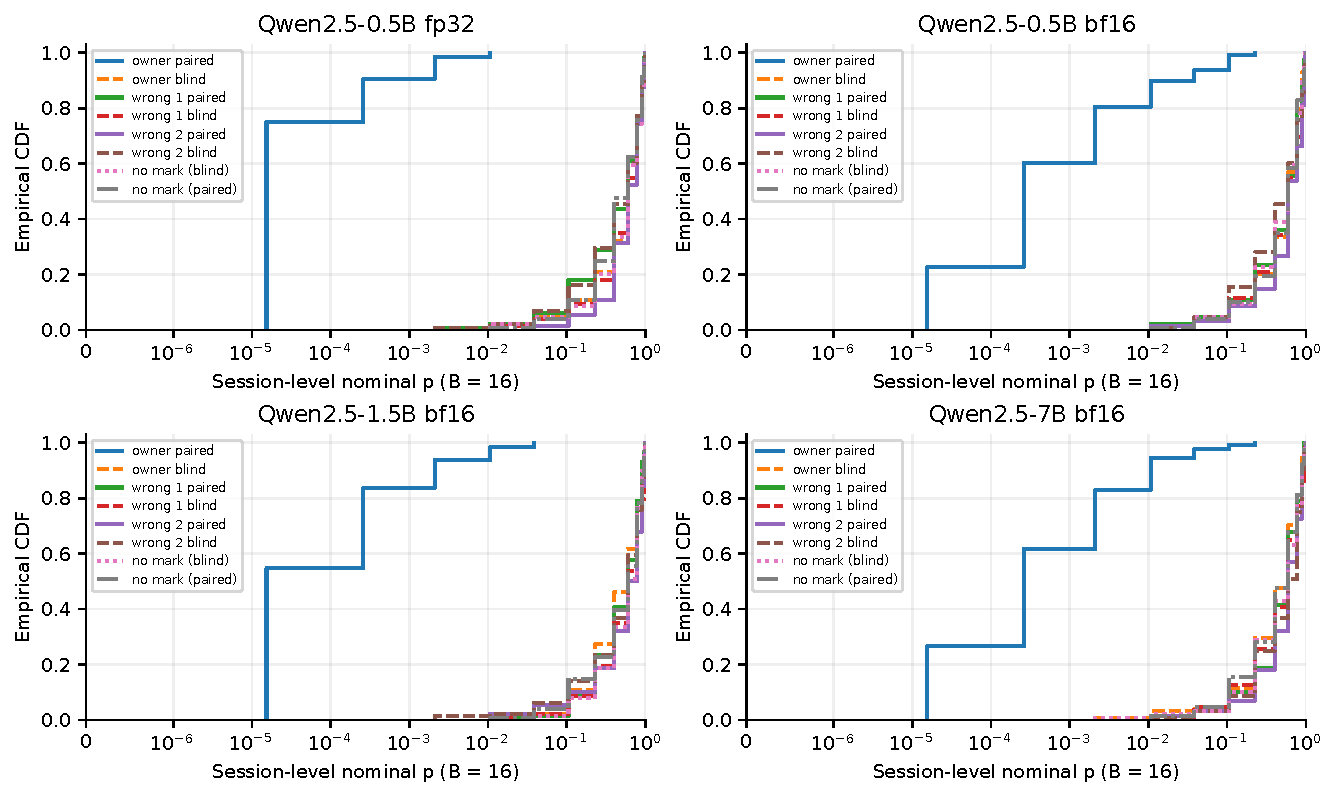
\includegraphics[width=.86\linewidth]{figures/session_p_ecdf.pdf}
\caption{Sixteen-physical-coordinate nominal-tail ECDFs: owner and two wrong keys, paired and blind; no-mark is blind and, when measured, paired.}\label{fig:ecdf}
\end{figure}
Substitution recovers all sixteen uncoded bits in every measured model. It matches
or exceeds honest paired recovery without carrying the mark through intervening
blocks. A near-identity local residual response is a plausible explanation, not a
measured Jacobian. The result excludes interpreting successful decoding as proof
of execution. Precommitment prevents later rewriting; it cannot make an earlier
fabrication truthful.

\section{Failure of the tested projected-logit decoder}
The legacy \texttt{watermark\_provenance\_result.json} probe used sixteen prompts
and eight prediction positions, not eight prompts. At $B=16$, $\alpha=0.01$, it
reports residual accuracy $\VoneResidual$, tested logit accuracy $\VoneLogits$,
KL $\VoneKL$ and token agreement $\VoneAgreement$.
\begin{figure}[htbp]\centering
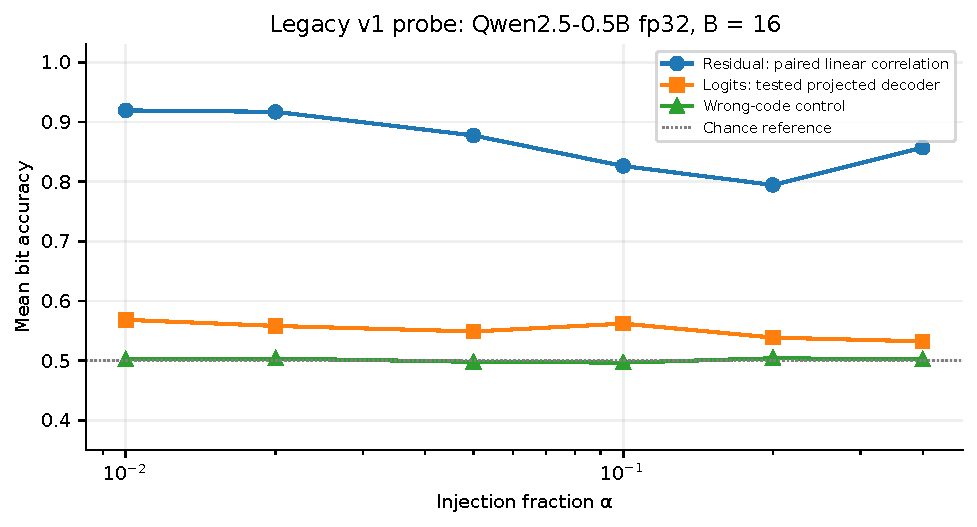
\includegraphics[width=.68\linewidth]{figures/logit_wall.pdf}
\caption{Legacy residual/logit recovery versus amplitude; not a long-rollout or blind-verification test.}\label{fig:wall}
\end{figure}
The logit decoder correlates differences against $WC_K$. Unembedding $W$ is linear;
final RMS normalization is nonlinear. Weak recovery by this decoder does not prove
all logit or text detectors impossible. No text-only detector is validated here.
The broader empirical study is companion Paper B,
\emph{Engineered CDMA superposition in pretrained transformers collapses at every
untrained non-linearity}~\citep{vargascompanion}.

\section{Related work}
\citet{kirchenbauer2023} favor pseudorandom green tokens and detect from text without
model parameters. Our activation-log tag has a different access model and does
not inherit that black-box guarantee. SEAL~\citep{seal2025} edits latent subspaces
for model-ownership watermarking with white-/black-box settings.
EverTracer~\citep{evertracer2025} uses fine-tuning and calibrated probability
variation for probabilistic model fingerprinting. Both concern model ownership,
not per-session audit labels. No robustness comparison is measured here.
Certificate Transparency~\citep{rfc6962} supplies append-only commitment machinery,
not truthfulness of logged statements. zkLLM~\citep{zkllm2024} instead constructs
zero-knowledge machinery to prove LLM computation. Its soundness target differs
from correlation with a secret activation code; activation tagging is not a
lightweight equivalent of verifiable inference.

\section{Limitations}
The experiments cover one prompt source, greedy decoding, one placement rule and
fixed public research seeds. They do not establish semantic fidelity, sampling
quality, paraphrase robustness or stability under fine-tuning. Model, tokenizer,
precision or kernel drift can break paired replay. The matched 0.5B experiment
shows that precision, rather than size, dominates the measured degradation; fixed
$\alpha=0.01$ is not precision-invariant. This attribution is limited to these
models and kernels, without additional amplitudes or repeated runs.
Only two wrong keys are tested;
physical null independence remains an assumption checked imperfectly by controls.
Logical majority votes have tie bias, and sixteen payload bits are not a unique
session identifier. Neither detection nor failure to detect proves origin or
non-origin against a malicious provider.

Capture integrity, logging completeness, retention, commitment privacy and
production costs require separate evaluation. Compact projections are not
zero-knowledge disclosures. Paired verification needs text privately. Signed
unmodified activation logs also support internal replay consistency without
perturbing generation. The incremental utility of the perturbation over that
baseline remains unproven; these experiments characterize the mechanism and its
negative results rather than establish a deployment advantage.

\section*{Reproducibility}
Repository: \url{https://github.com/ttzrs/neural-cdma}. Previous publication:
\href{https://doi.org/10.5281/zenodo.20570543}{10.5281/zenodo.20570543}, a concept DOI
resolving to v1 record \href{https://doi.org/10.5281/zenodo.20570544}{20570544}
\citep{vargasv1}. Neither identifies this revision.
\texttt{watermark\_scale.py} defines the current experiment;
\texttt{watermark\_provenance.py} supports the legacy probe.
Table~\ref{tab:revisions} identifies exact model revisions. New JSONs record
\texttt{config.model\_revision}; the earlier snapshots are listed explicitly.
The experiment saves decoding statistics, not the committed tuple in
Eq.~\eqref{eq:record}. Publishing reproducible committed tuples remains future work.
% Generated by make_tables.py; do not edit.
\begin{table}[htbp]
\centering
\small
\begin{tabular}{lp{.58\linewidth}l}
\toprule
Model/dtype & Hugging Face model revision & Provenance \\
\midrule
0.5B fp32 & \path{060db6499f32faf8b98477b0a26969ef7d8b9987} & legacy snapshot \\
0.5B bf16 & \path{060db6499f32faf8b98477b0a26969ef7d8b9987} & legacy snapshot \\
1.5B bf16 & \path{8faed761d45a263340a0528343f099c05c9a4323} & legacy snapshot \\
7B bf16 & \path{d149729398750b98c0af14eb82c78cfe92750796} & legacy snapshot \\
\bottomrule
\end{tabular}
\caption{Model revisions. Legacy snapshots identify the earlier runs whose JSONs omitted this field; new JSON revisions take precedence.}\label{tab:revisions}
\end{table}

Run \texttt{bash build.sh} in \texttt{papers/forensic/} to regenerate tables,
figures, BibTeX references and PDF. Numeric claims use generated macros; full
source hashes are in \path{tables/source_manifest.json}. The package's demonstrative
reinjection verifier is distinct from the committed-record protocol specified here.

\begingroup\small
\bibliographystyle{plainnat}
\bibliography{refs}
\endgroup
\appendix
\section{Changes from version 1}
\begin{table}[htbp]\centering\small
\begin{tabular}{p{.17\linewidth}p{.32\linewidth}p{.40\linewidth}}
\toprule
Issue & v1 & This revision\\
\midrule
Prompts & ``8''; actually $16\times8$ positions & Separate session/calibration counts\\
Protocol & Static formula, paired code & Separate paired and blind definitions\\
Statistics & Pooled deltas & Per-session physical detection; logical recovery\\
Fidelity/claim & Short agreement; non-repudiation & Long divergence; committed-record consistency\\
\bottomrule
\end{tabular}
\caption{Changes from the previous version.}\label{tab:corrections}
\end{table}
\end{document}
